\documentclass[11pt]{article}
\usepackage{lmodern}

% ---------- Layout ----------
\usepackage[letterpaper,margin=1in]{geometry}
\usepackage{setspace}
\setstretch{1.05}

% ---------- Math & text ----------
\usepackage{amsmath,amssymb}
\usepackage{microtype}

% ---------- Figures & tables ----------
\usepackage{graphicx}
\usepackage{float}
\usepackage{array}
\usepackage{caption}
\usepackage{subcaption}
\usepackage{placeins}
\usepackage{longtable}
\usepackage{booktabs}
\usepackage{threeparttable}       % NEW: table notes
\usepackage{siunitx}              % NEW: S columns for decimal alignment
\usepackage{pdflscape}


% ---------- Bibliography ----------
% natbib MUST be loaded BEFORE hyperref
\usepackage[authoryear]{natbib}

% ---------- Links ----------
% hyperref should be loaded after all other packages (except cleveref)
\usepackage[colorlinks=true,linkcolor=blue,citecolor=blue,urlcolor=blue]{hyperref}

% ---------- Smart cross-references ----------
% cleveref MUST be loaded AFTER hyperref
\usepackage{cleveref}             % NEW: \cref and \Cref commands

% ---------- Notation macros (00S Symbology and Notation Lock) ----------
\newcommand{\mut}{\mu_t}
\newcommand{\chit}{\chi_t}
\newcommand{\kapt}{\kappa_t}
\newcommand{\knrc}{k^{\text{NRC}}}
\newcommand{\kme}{k^{\text{ME}}}
\newcommand{\Ypot}{Y^{p}}
\newcommand{\mech}{q}
\newcommand{\pkap}{p_t^{\kappa}}
\newcommand{\impint}{\nu}
\newcommand{\deprec}{\delta}
\newcommand{\discard}{z}
\newcommand{\stepD}{\boldsymbol{\gamma}'\mathbf{D}_t}
\newcommand{\stepDsys}{\boldsymbol{\Gamma}\mathbf{D}_t}
\newcommand{\MPF}{Mechanization Productive Frontier}

% ---------- Placeholder marker ----------
\newcommand{\PLACEHOLDER}[1]{%
	\par\medskip\noindent\fbox{\parbox{0.96\linewidth}{%
			\footnotesize\textbf{[PLACEHOLDER]}~#1}}\par\medskip}
% ---------- Title block ----------
\title{The Transformation of Accumulation into Productive Capacities: Capacity Utilization in the Center and Periphery\thanks{This paper benefited from AI-assisted editing for syntax refinement, structural suggestions, and stylistic consistency checks. All analytical arguments, historical interpretations, and substantive content remain the author's sole responsibility.}\\
\begin{large}
\textbf{WORK IN PROGRESS / PLEASE DO NOT CIRCULATE}     
\end{large}
}
\author{Diego Polanco\thanks{Doctoral Candidate in Economics, Department of Economics, University of Massachusetts Amherst.}\\
Department of Economics, University of Massachusetts Amherst\\
\texttt{dpolanconeco@umass.edu}}
\date{\today}

\begin{document}
\maketitle

\begin{abstract}

\end{abstract}

\vspace{1cm}

\noindent\textbf{Keywords:} Capacity Utilization; Transformation Elasticity; Choice of Technique; Cointegration; Marx-Okishio; External Balance; Center-Periphery.

\noindent\textbf{JEL Codes:} B51; C32; E01; E22; E32; P16.

\pagebreak

\FloatBarrier
\section{The Unresolved Problem of Capacity Utilization}

\paragraph{A}
This paper examines how the rate of profit, capital accumulation, and productive capacity formation interact under conditions of distributional conflict between labor and capital.

\paragraph{B}
\PLACEHOLDER{Section 1 is unwritten. What exists above is a single orienting sentence; the section that the locked outline requires does not yet exist. The remainder of this box states what it has to do, so the gap is legible rather than silent.}

\paragraph{C}
\PLACEHOLDER{\textbf{Burden of the section.} Establish that capacity utilization is unresolved in the treatments that have come down to us, in three distinct ways, and show that these are three faces of one problem rather than three separate difficulties. First, utilization treated as a \emph{given macro ratio}: taken as observed when its denominator is not. Second, utilization treated as an \emph{inherited benchmark}: anchored to an engineering or survey norm imported from outside the accounting framework that is supposed to give it meaning. Third, utilization treated as an \emph{empirical residual}: whatever is left after output has been fitted to capital, which presupposes the very transformation relation at issue. The third case is where the filtering literature sits, and the objection to it here is structural rather than methodological --- a filter that fits output to capital imposes a unit transformation elasticity by construction, and so conflates utilization with the object that would be needed to identify it. That argument is available from this chapter's own accounting framework and requires no external authority.}

\paragraph{D}
\PLACEHOLDER{\textbf{Bottom line up front.} Per the writing calibration in force, the contribution must be visible by the end of the second paragraph: what the paper examines, how it identifies the transformation elasticity, and what the comparison of the United States and Chile establishes. The reader should not have to reach Section 3 to learn what is being claimed.}

\paragraph{E}
\PLACEHOLDER{\textbf{What must not appear here.} Long literature catalogues. The full center--periphery discussion, which belongs in Section 5. Estimator debates, which belong in Section 4 and Appendix C. Detailed methodological caveats. The section motivates a problem; it does not litigate the solution.}

\paragraph{F}
\PLACEHOLDER{\textbf{Closing-line burden (locked).} The section must arrive at: \emph{the utilization problem cannot be resolved at the level of the ratio alone; it must be reconstructed through the relation that governs productive-capacity formation.} This hands off directly to Section 2.}

\paragraph{G}
\PLACEHOLDER{\textbf{Also unresolved: the abstract's sample window.} The abstract states a United States window of 1947--2024, while Sections 4 through 6 estimate over 1929--2024 with MATHPLACEHOLDER0XYZ. The two cannot both be right. Note further that 1929--2024 spans 96 years against a reported MATHPLACEHOLDER1XYZ of 94, and that the estimation prose elsewhere gives the effective span as 1931--2024 after lag-1 conditioning and listwise deletion --- which is consistent with MATHPLACEHOLDER2XYZ and suggests the table titles, not the sample, are what needs correcting.}
\FloatBarrier
\section{The Internally Divided Firm and Capacity Formation}

\paragraph{2.1} Capacity utilization is not a technical parameter. It is an
inter-scalar political-economic settlement. The macroeconomic
capacity ceiling---the denominator of the utilization rate---is
not a neutral engineering constraint but a historically contingent
outcome conditioned by the balance of class power. Yet identifying
this distributional conditioning at the macro level leaves the
underlying transmission mechanism black-boxed: how, precisely,
does distributive conflict physically alter the conversion of
accumulated capital into productive capacity?

\paragraph{2.2} Answering this question requires dismantling a hidden premise
shared by virtually all heterodox growth models: the unified
firm. Whether treating the normal rate of capacity utilization
as an endogenous behavioral target or an exogenous gravitational
anchor, standard frameworks presume a coherent organization
capable of selecting a utilization benchmark, enforcing it across
the labor process, and sustaining it over time. Formally, the
utilization rate is defined as:
%
\begin{equation}\label{eq:utilization}
	\mu_t \equiv \frac{Y_t}{Y^p_t},
\end{equation}
%
\paragraph{2.3} \noindent where $Y_t$ is realized output and $Y^p_t$ is potential
productive capacity. But this ratio conceals a deeper question:
who determines $Y^p_t$, and under what organizational conditions?

\paragraph{2.4} The unified-firm premise collapses when confronted with the
social organization of capitalist production. In a decentralized
economy, individual capitals commit fixed investments without
\textit{ex-ante} coordination, confronting one another in
competitive markets. Within the enterprise, production decisions
encounter contradictory managerial and worker imperatives.
Capacity utilization cannot be reduced to a target selected by
a single optimizing entity. To theorize the political economy
of productive capacity, we replace the unified firm with two
interconnected frameworks: Okishio's theory of decentralized
market anarchy, and Vidal's theory of the internally divided
firm.

\subsection{Smooth Reproduction and the Unified-Firm Premise}

\paragraph{2.5} Proportional reproduction is a condition of feasibility, not a
tendency of capitalist accumulation. Smooth reproduction requires
strict material proportionality between departments of
production---a condition \citet{Basu2022} and \citet{Okishio2022} formally established defined by the latter as the equilibrium accumulation trajectory. \citet{Bergmann2009} call
this balanced trajectory, where realized output meets productive
capacity ($\mu_t = 1$), the \textit{``golden path.''} But the golden path
is a methodological closure, not a gravitational attractor. It
identifies the conditions under which realization can reproduce
itself smoothly; it does not describe the path capitalist accumulation
actually follows. Neither the post-Keynesian assumption of long-run balanced
growth \citep{BleckerSetterfield2019} nor the \textit{``Keynesian in the short run, classical in the long run''} synthesis \citep{DumenilLevy1999} captures this persistence of unbalanced expansion.

\paragraph{2.6} Nothing in the logic of decentralized competition
establishes that private investment decisions will reproduce
these proportions. A stylized illustration makes the point
concrete. If productive capacity grows at $5\%$ per year while
aggregate demand for output grows at $2\%$, capacity outpaces
demand by three percentage points each year. After a decade,
utilization falls to roughly $75\%$ of capacity---not because
of a temporary shock, but because uncoordinated investment
persistently builds capacity faster than demand can absorb it.
Balanced growth ($g_Y = g_K$) is merely one configuration of
the transformation elasticity $\theta$; it is not a restoring
force. Smooth reproduction ($\mu_t = 1$) does not require
$\theta = 1$; it holds for any transformation elasticity.
Balanced growth is the narrower special case in which
$\theta = 1$ and $\mu_t = 1$ coincide in the long run.

\paragraph{2.7} Because private investment decisions are made without
\textit{ex-ante} coordination, real capitalist economies
routinely violate the proportional conditions of the golden path.
\citet{Okishio2022} demonstrates that chronic disproportionality
is not a temporary friction but the structural norm of
decentralized accumulation. Treating the transient benchmark of
$\mu_t = 1$ as a behavioral target therefore relies on a hidden
premise: that the firm is a unified planning subject capable of
selecting a utilization norm, enforcing it across the labor
process, and sustaining it over time. This premise---the unified
firm---is the target of the present section.

\paragraph{2.8} The denominator of the utilization ratio (productive capacity
$Y^p_t$) is not an engineering constant. It is a contested
settlement of divided management and shop-floor struggle. The
numerator (realized output $Y_t$) is hostage to the anarchy of
demand. Smooth reproduction supplies a reference case against
which this historical non-coincidence can be studied. It does not
supply the mechanism that produces it.

\subsection{Decentralized Accumulation and Market Anarchy}

\paragraph{2.9} If the ``golden path'' of smooth reproduction is merely a
benchmark of feasibility, the actual trajectory of capitalist
accumulation is governed by the decentralized organization of
investment. Capitalist production is coordinated through
exchange, meaning that the social validation of private
decisions occurs only \textit{ex-post}. Because money mediates
exchange, sale and purchase are separated moments of the capital
circuit \citep{Basu2022}. Surplus value must be realized in
circulation, not by construction \citep{Foley1985, Trigg2020}.
This constitutes the logic of capital as impersonal domination:
capitalists commit to production and investment with the law of
value operating \textit{``behind their backs.''}\footnote{Karl
	Marx, \textit{Capital}, Volume~I, Chapter~1, Section~4 (\textit{``The
	Fetishism of Commodities and the Secret thereof''}), where the
	law of value operates as an overriding law of nature when
	private producers exchange products \citep{MarxKVI}.} They are subject to market
forces and value relations they neither control nor consciously
direct. Critically, this anarchy is not a coordination failure
in an otherwise functional market. The market is a socially
constituted institution whose normal operation produces
disproportionality as a structural feature
\citep{VidalPeck2012}. \citet{Okishio2022} locates the source
of macroeconomic instability precisely in this constitutive
anarchy. Individual capitals commit to fixed investment on the
basis of private profititability expectations, yet the market validates
those commitments only after production has begun. No firm can
know in advance whether its expansion fits the investment and
consumption decisions taken elsewhere. The coordination problem
is not one of imperfect information surrounding an otherwise
coherent plan; no economy-wide plan exists.

\paragraph{2.10} Smooth reproduction requires proportional expansion across
sectors producing means of production and sectors producing
consumption goods. Because private investment does not enforce
this proportionality, firms extrapolate past prices, profit
rates, and sales. A signal that induces expansion in one branch
routinely produces excess capacity before complementary demand
materializes elsewhere. Contraction works through the same
cumulative mechanism: falling sales cut investment, reducing
aggregate demand and validating further cuts. Removing Say's
Law reintroduces realization as a substantive condition of
reproduction: accumulation may generate capacity that demand
fails to absorb, or demand may temporarily exceed productive
capacity \citep{Foley1985}. Prices register the
resulting imbalance, but they do not prevent the sunk
commitments produced by it.


\paragraph{2.11} Fixed capital gives this temporal lag its structural force.
Structures and machinery embody long-horizon commitments that
cannot be reversed when relative prices or demand conditions
shift. Once installed, excess capacity leaves the firm to
operate below its anticipated scale, defer maintenance, hold
equipment idle, or devalue the asset. These responses
distribute the costs of market anarchy among firms, workers,
and creditors, but they do not restore the missing
\textit{ex-ante} coordination.

\paragraph{2.12} Idle capacity is therefore a recurrent, structural form of
decentralized accumulation rather than a temporary friction.
Private investment physically builds capacity before the market
can realize its social use, recurrently a gap
between installed productive capacities ($Y^p_t$) and effective demand ($Y_t$). The capacity utilization rate ($\mu_t$) registers this gap at the macro level. Unbalanced growth is not a disturbance around proportionality; it is the structural consequence of distributively conditioned investment under
decentralized decision-making. The analytical problem is
therefore not how proportionality re-emerges, but how persistent
imbalance remains historically reproducible. The condition
$\mu_t = 1$ is at most a transient point through a given trajectory
proportionality, while persistent divergence records the ongoing
reality of market anarchy.

\paragraph{2.13} Yet Okishio's macro framework leaves a crucial gap: it does not explain how firms translate this external anarchy into internal operating decisions. The firm does not manage market anarchy; it internalizes it. A firm does not receive a price signal and respond as a frictionless, unified unit. It processes the signal through an organization divided over control, cooperation,
effort, and the allocation of resources. Vidal's internally
divided firm provides that missing mediation.

\subsection{The Internally Divided Firm}

\paragraph{2.14}

Vidal builds on Marx's Volume~I theory of the labor process, drawing on contemporary organizational theory and sociological institutionalism to develop an organizational political economy of the capitalist firm \citep{VidalPeck2012, Vidal2022}. Marx established that
capitalist management faces a constitutive contradiction: it
must simultaneously organize the cooperative labor required for
production and enforce the coercive control required for
valorization. \citet{Vidal2022} demonstrates how this contradiction fractures
the modern capitalist firm, treating it as a divided social
organization whose internal structure is shaped by cognitive,
normative, regulative, and organizational institutions. Management must extract surplus value through
control over labor, but production also requires workers'
cooperation, tacit knowledge, and problem-solving capacity.
Standardization and surveillance secure a measurable pace of
work while weakening the discretion needed to sustain complex
production. The firm cannot maximize both imperatives at once
because the labor process that produces value is also the site
where workers contest its extraction. This contradiction is not
a universal constant of capitalism; it is institutionally
mediated, taking variegated forms across distinct accumulation regimes throughout historical capitalism
\citep{Vidal2019}.

\paragraph{2.15}
Workers respond to this contradiction by actively calibrating
effort, cooperation, machine pacing, and the deployment of tacit
knowledge. Capitalist management extracts potential capacity
through concrete shop-floor mechanisms: increasing machine speed,
deferring maintenance to hit short-term throughput targets, and
enforcing rigid surveillance. Workers contest this extraction
through labor turnover, collective exit, or the deliberate
withdrawal of problem-solving cooperation and effort. Throughput,
quality, and maintenance therefore depend on social relations
that no engineering specification fixes in advance. A production
target that raises machine speed by deferring maintenance may
increase current output while degrading sustainable capacity. A
directive that suppresses worker discretion may meet a
short-term labor-control objective while worsening workflow
bottlenecks. Labor effort is consequently not a fixed technical
parameter applied to a pre-existing capital stock; it is an
active, contested determinant of the capacity utilization itself.

\paragraph{2.16}
This dynamic enforces a strict wedge between
\textit{engineering capacity} and \textit{practical capacity}.
Engineering capacity records the theoretical maximum output of
equipment under ideal technical conditions. Practical capacity
records the sustainable output rate dictated by actual
maintenance schedules, product-mix complexity, and the negotiated
intensity of labor. When managers report capacity to national
statistical agencies, they rely on conventions shaped by their
organizational position and the immediate pressures of the shop
floor. Aggregate capacity statistics therefore do not reveal a
neutral physical ceiling; they aggregate situated, institutional
judgments \citep{Shaikh2016, Nikiforos2016}. Complementarily,
empirical surveys of managerial practice confirm that firms do
not systematically organize production decisions around a
coherent capacity utilization target \citep{Singh2022}. For the
purposes of macroeconomic modeling, the productive capacity
ceiling ($Y^p_t$) is not an exogenous engineering constraint but
an endogenous settlement of workplace conflict. This settlement
is the micro-foundation through which class struggle and
distribution transmit into capacity utilization, setting up the
distributive--technological mapping developed in the following
subsection.

\paragraph{2.17}
Because the valorization--labor process contradiction cannot be
solved, firms settle into organizational configurations of
\textit{``mediocre sufficiency''} \citep{Vidal2022}. These are hybrid
arrangements that reproduce production without resolving the
underlying conflict between control and cooperation. Partial
worker autonomy coexists with rigid discipline; continuous
improvement programs coexist with brutal throughput pressure;
machinery might remain idle alongside binding productive bottlenecks. Following
\citet{Vidal2014}, these arrangements are best understood as
\textit{institutional incoherence}: the firm's internal
settlements are functional enough to sustain accumulation yet
contradictory enough to generate persistent friction. This stands
in direct contrast to the Varieties of Capitalism assumption of
institutional complementarity, where national institutions are
presumed to form coherent, mutually reinforcing systems \citep{Hall2003}. Here,
incoherence is not a deviation from an optimizing norm; it is the
permanent, structural form through which capitalist management
physically converts accumulation demand into capacity usage. 

\subsection{Distribution, Technique, and the Transformation
	of Accumulation}

\paragraph{2.18}
The choice of technique connects the divided firm to
distribution, governing how accumulated capital is physically
transformed into productive capacity. Capitalists adopt a new
technique only when it reduces the cost of production at
prevailing prices and wages; such a technique is capitalistically
viable \citep{Okishio1961}. \citet{Okishio1961} demonstrates
that a viable capital-using, labor-saving (CU-LS) technique
raises the equilibrium profit rate when the real wage remains
constant---a direct challenge to Marx's law of the tendential
fall in the rate of profit. Marx's account, by contrast, allows
the same form of technical change to depress profitability when
rising capital intensity increases the capital advanced relative
to surplus value. \citet{Basu2022} formalizes the
Marx--Okishio threshold: the rate of real-wage growth that
separates these outcomes. It is a distributive boundary set by
the balance of class forces, not a technical constant.

\paragraph{2.19}
This boundary situates the present framework within the
induced-innovation tradition while departing from it. The
Innovation Possibility Frontier (IPF) literature, initiated by
\citet{Kennedy1964}, treats distribution as selecting the
\textit{direction} of technical change along a given frontier:
relative factor costs determine whether innovation is
labor-augmenting or capital-augmenting, while the frontier
itself---the scale of feasible productivity growth---remains
exogenous \citep{Julius2005, Tavani2012}. Later assessments
sharpen this limitation: IPF-based models explain the
composition of technical change but remain largely silent on
innovation intensity \citep{TavaniZamparelli2018}.
\citet{Zamparelli2024a} partially endogenizes scale by mapping
a family of IPF levels to R\&D effort, yet the analytical
structure continues to rely on frontier geometry and
steady-growth closure \citep{Zamparelli2024b}. An alternative
strand reframes inducement through mechanization rather than
frontier selection: \citet{Kaldor1957} links productivity
growth to capital deepening, while
\citet{CajasGuajirro2024} reformulates the IPF with an explicit
choice over mechanization growth under distributive and
labor-market conditions. The present framework builds upon a 
mechanization productive frontier,  treating the distributive--technological 
relation as a regime-specific transformation between accumulation and
productive capacity. Rather than selecting along a given
frontier, distribution conditions mechanization intensity,
which in turn determines the transformation elasticity linking
accumulation to the formation of productive capacities. 

\paragraph{2.20}
The Marx--Okishio threshold gives wage pressure a precise role
in mechanization, but the profitability outcome depends on the
labor market closure. \citet{Basu2026} demonstrates that the
equilibrium profit rate after viable CU-LS technical change is
governed by the institutional structure of capital--labor
bargaining. Under a constant-wage-share closure---what
\citet{Basu2026} formalizes as the ``strong labor'' regime,
applicable to Atlantic Fordism---any viable CU-LS technique
unambiguously \textit{lowers} the equilibrium profit rate.
Marx's LTFRP reigns supreme precisely where labor is powerful
enough to compel real wages to grow in tandem with productivity.
Under this closure, rapid mechanization is induced by
distributive pressure, yet the same pressure contests capital's
claim on the resulting productivity gains
\citep{Vidal2015, Vidal2019}. A stylized illustration makes the
mechanism concrete. If a $10\%$ real wage increase raises
mechanization intensity by $8\%$ under strong-labor conditions,
the transformation elasticity $\theta$ rises from $0.70$ to
$0.85$: accumulation translates more efficiently into productive
capacity because firms substitute machinery for labor. Wage-led
mechanization was not a harmonious productivity bargain; it was
a contested settlement in which the distributive pressure that
induced technical change simultaneously eroded the profit rate
it was meant to restore.

\paragraph{2.21}
The weakening of organized labor after the Fordist crisis
altered that mechanism. Under the ``weak labor'' closure---where
the unemployment rate remains constant and workers lack the
institutional power to enforce a target wage share---the
distributive pressure to replace labor is suppressed
\citep{Basu2026}. Yet mechanization does not cease. Lower
relative machinery prices and technical change in capital-goods
production continue to favor capital-using techniques through a
second, independent channel. Distribution and machinery prices
therefore constitute a dual-channel mechanism in the
choice of technique. Their relative force changes across
accumulation regimes, which prevents the wage share from being
treated as an external control added to an otherwise autonomous
technical relation. Extending the stylized example: under
Post-Fordist conditions, a $15\%$ decline in relative machinery
prices raises mechanization intensity by $6\%$, partially
compensating for the weakened distributive channel and
sustaining $\theta$ near $0.75$ despite wage suppression. The
same $10\%$ wage increase that produced an $8\%$ mechanization
response under Fordism produces only a $2\%$ response under
Post-Fordism, leaving $\theta$ near $0.72$. The two channels do
not simply add; they interact through the institutional
configuration that governs their relative force.

\paragraph{2.22}
These channels still operate through the contradictions
identified in the preceding subsections. Firms choose techniques
before demand validates the associated capacity, and they
operate those techniques through labor processes that divide
control from productive cooperation. Investment consequently
does not translate one-for-one into a stable productive ceiling.
The transformation depends on the composition of capital, the
distributive conditions governing mechanization, and the
organization through which installed equipment becomes usable
capacity. In a labor surplus economy---the third closure
identified by \citet{Basu2026}, applicable to peripheral
capitalism---the real wage remains constant and the equilibrium
profit rate rises unambiguously after viable CU-LS technical
change. Yet the peripheral transformation is structurally
truncated by external financial subordination and the balance of
payments constraint, a mechanism developed in the following
subsection.

\paragraph{2.23}
Okishio and Vidal jointly rule out any direct, automatic
passage from accumulation to productive capacity.
Decentralized investment generates structural
disproportionality across firms and sectors; the internally
divided firm internalizes this disproportionality as
contested operating conditions rather than a coherent
utilization target. The analytical object that captures this
mediated transformation is the \textit{transformation elasticity} ($\theta \equiv d y^p / d k$), which governs how
accumulation converts into productive capacity under
distributive conflict and market anarchy. The empirical
analysis bounds this multi-sector mechanism to a
single-sector aggregate, masking internal sectoral
divergences while preserving the core transformation logic.
Section 3 formalizes $\theta$ within a regime-specific
analytical framework and derives its econometric
implications through structural change controls.


\subsection{Historical Regimes of Institutional Mediation and the Transformation Elasticity}

\paragraph{2.24}
The transformation elasticity is not a fixed
engineering parameter. It is an emergent property of class
struggle and the prevailing institutional environment.
Decentralized accumulation does not automatically guarantee
proportional reproduction ($\theta = 1$). Institutional
mediation---wage-setting norms, financial architectures, and
competitive structures---conditions how distributive pressures
translate into mechanization choices
\citep{Aglietta2000, VidalPeck2012}. Shifts in this
mediation across historical periods will not be imposed
through ex ante sample splits. The empirical strategy
identifies them endogenously through structural change
controls and break dummies, allowing the data to reveal how
institutions bounded structural drift without requiring a
formal equilibrium closure.

\paragraph{2.25}
\citet{Basu2026} demonstrates that the equilibrium profit
rate after viable capital-using, labor-saving (CU-LS)
technical change is governed by the labor market closure,
which maps directly onto distinct historical accumulation
regimes. Under a \textit{constant-wage-share} closure---the
institutional signature of Atlantic Fordism
(1947--1973)---workers possess the bargaining power to grasp
productivity gains, forcing real wages to grow in tandem with
labor productivity. In this strong-labor regime, viable
mechanization unambiguously lowers the equilibrium profit
rate, so that Marx's law of the tendential fall in the rate
of profit holds \citep{Basu2026}. This stagnation tendency
was institutionally offset: the class compromise, mass
consumption, oligopolistic market structures, and military
Keynesianism of the Fordist era absorbed the surplus and
sustained effective demand \citep{Vidal2019}.

\paragraph{2.26}
Under a \textit{constant-unemployment} closure---which resembles the persistent unemployment feature of the post-Fordist accumulation regime---an era during which the class compromise that took place during the Fordist period is dismantled and labor's
bargaining power is severely weakened. The wage share falls,
and mechanization is driven not by distributive pressure but
by the relative cheapening of ICT and the shift toward
financially reversible, short-horizon assets, patents and intellectual property of untangible assets 
\citep{Lapavitsas2011, Pagano2014}. Because wages no longer
track productivity, the profit rate may stabilize or rise,
but the suppression of wage-led demand generates a chronic
under-consumptionist stagnation tendency. Following \citet{Vidal2019}, I hypothesize that under structural conditions, the post-fordist accumualtion regime produces a dysfunctional utilization configuration:
accumulation decouples from productive capacity formation,
generating chronic idle capacity that is temporarily masked
by debt-led consumption and financial fragility rather than
sustainable realization \citep{Stockhammer2012, Vidal2019}.

\paragraph{2.27}
In the capitalist periphery, different closures represent distinct historical configurations throughout Chilean history. First, under an assumption of a
\textit{constant-real-wage}, which corresponds to
Okishio's original formulation maps onto a surplus-labor
economy \citep{Lewis1954, Basu2026}. During the
import-substituting industrialization (ISI) era, the
\textit{rural-urban} and \textit{demographic} transition enabled by the transformation of sanitary conditions and a massive drop of child moratlity in the early XX century,  regulated late industrialization, providing an unlimited supply of labor from the countryside that disciplined urban wages and allowed the profit rate to reproduce itself alongside mechanization. 
However, peripheral mechanization is structurally import-biased:
widening the mechanization gap requires imported capital
goods and technologically non-substitutable inputs
\citep{Prebisch1981}. The balance of payments constraint
therefore acts as a hard external ceiling on the
transformation of accumulation into capacity. Under a
developmentalist regime with surplus labor (1933--1957), this operated as an
\textit{import capacity ceiling}. Second, a \textit{constant-wage-share} or more accurately \textit{rising-wage-share} closure, represents the intensification of stagnation tendencies leading to structural crisis of capitalism once the unlimited supply of labor depleted and the incentives for capitalist firms to mechanize risen due distributive pressures while increasing imnport requirements and stressing further the external constraint. Third, the discipline imposed by the neoliberal counter-revolution \citep{Casals2021} (1974--present) a \textit{constant-unemployment} closure coupled with trade and capital account liberalization relieved the external constraint, but locked the periphery into extractive specialization and premature deindustrialization, such that the WTO and bilateral free
trade agreements legally encoded a \textit{policy space ceiling} \citep{Ahumada2019, Palma2019}.


\paragraph{2.28}
These historical configurations establish that the productive
ceiling is not a neutral, trans-historical engineering
constraint but a contingent outcome of decentralized
accumulation, class power, and a country's relative
positionality within the capitalist world system. The
center--periphery comparison reveals a fundamental asymmetry:
in the center, structural crises arise from the
\textit{exhaustion} of institutional mediation (e.g., the
1970s profit squeeze); in the periphery, crises arise from
the \textit{absence} of sovereign mediation and 
truncation by global financial markets causing regime shifting behaviors under external imbalances. The immediate task
is to translate these historical-institutional claims into a
formal analyitical architecture. Section 3 formalizes
induced technological change under a cost-minimization
problem, first advanced by \citet{CajasGuajirro2024}, in
three stages of increasing complexity: i) aggregate
capital-deepening; ii) mechanization bias under heterogeneous
capital decision-making; and iii) a peripheral
foreign-exchange bottleneck that induces technological change
through mechanization. These analytical foundations provide
the toolkit to deploy an empirical strategy identifying a
state-dependent $\theta$ parameter endogenous to
distributive conflict, tracing the trajectory of productive
capacities and the capacity utilization ratio through a
structural empirical approach.

\FloatBarrier
\section{The Analytical Framework: Formalizing the
	Transformation Elasticity}
\label{sec:3:analytical_framework}

\paragraph{3.0}
This section translates the distributive--technological
mechanism of Section~2 into a formal model that yields
estimable restrictions. \citet{CajasGuajirro2024} first
advanced the cost-minimization problem over mechanization
growth; I extend it through three subsections of
increasing complexity. Section~3.1 formalizes aggregate
capital-deepening under Leontief technology and derives
the transformation elasticity $\theta$ endogenously from
the cost-minimizing choice of technique. Section~3.2
unbundles aggregate capital into extensive nonresidential
structures and intensive machinery, and derives the
state-dependent mechanization gap $\kappa_t$ under a
dual-channel viability condition. Section~3.3 imposes the
peripheral foreign-exchange bottleneck as a binding
constraint on $\kappa_t$, generating a corner solution
that truncates $\theta$. Each subsection nests the
preceding one: setting the heterogeneity parameter to
zero recovers the baseline model; relaxing the
foreign-exchange constraint recovers the center model.
The empirical analysis bounds this multi-sector mechanism
to a single-sector aggregate, which masks internal
sectoral divergences but preserves the core transformation
logic. Section~3.4 synthesizes the theoretical claims of
the three models. Section~4 consolidates the
identification strategy and derives the cointegrating
specifications.

\subsection{The Baseline Model of Cost-Minimizing
	Mechanization (Homogeneous Capital Stock)}

\paragraph{3.1}
Actual aggregate output is represented by a Leontief
production function with fixed technical coefficients:
\begin{equation}
	Y = \min\left( A L,\; \mu B K \right)
	\label{eq:31:leontief}
\end{equation}
where $A = Y/L$ is actual labor productivity, $\mu = Y/Y^p$
is capacity utilization, and $B = Y^p/K$ is maximum capital
productivity. This production structure governs the rate of
profit through the fundamental heterodox accounting identity:
\begin{equation}
	r = \mu B (1 - \omega)
	\label{eq:31:profit_identity}
\end{equation}
where $\omega$ is the wage share. Standard macroeconomic
models treat $B$ as an exogenous technological given and $\mu$
as a behavioral constant smoothly targeted by a unified firm.
I reject both assumptions. The components of
\eqref{eq:31:profit_identity} are endogenous outcomes of
class struggle and decentralized market anarchy, as
established in Section~2. This subsection formalizes how
distributive pressure forces cost-minimizing firms to alter
their choice of technique, endogenously determining $B$.

\subsubsection{Tactical Choice of Technique and Induced
	Innovation}

\paragraph{3.2}
Capitalits firms choice of technique is given by aiming a mechanization growth rate $q$ under competitive cutting cost-pressures, looking at the net productivity surplus of technical change as their objective function.  Let $a$ denote the growth rate of
labor productivity. The effective distributive cost of
deploying mechanization growth is $q(1-\omega)$. Hence, the choice of technique of capitalist mechanization can be represented by: 
\begin{equation}
	\min_{q}\; c(q) = q(1-\omega) - a 
	\label{eq:31:objective}
\end{equation}
This objective captures the induced-innovation logic: firms
accelerate mechanization to expand labor productivity growth,
but the distributive cost of capital intensity holds them
back. The cost-minimizing objective function of capitalist becomes constrainted by a mechanization function that can be represented as:

\begin{equation}
	a = \Phi(q) = \lambda_0 + \lambda_1 q + \lambda_2 q^2
	\label{eq:31:frontier}
\end{equation}

\paragraph{3.3}
\textbf{Assumption 1.} \textit{Concavity of the
	mechanization frontier.} The frontier parameters satisfy
$\lambda_0 > 0$, $\lambda_1 > 0$, and $\lambda_2 < 0$. The
base productivity growth $\lambda_0$ sets the floor without
advanced machinery. The linear coefficient $\lambda_1$
captures the direct productivity payoff of mechanization. The
strict concavity $\lambda_2 < 0$ ensures diminishing marginal
returns to mechanization.

\paragraph{3.4}
Substituting \eqref{eq:31:frontier} into
\eqref{eq:31:objective} and solving the first-order condition
yields the optimal mechanization growth:
\begin{align}
	c(q) &= \lambda_0 + \left[\lambda_1 - (1-\omega)\right] q
	+ \lambda_2 q^2 \label{eq:31:unconstrained} \\
	\frac{\partial c}{\partial q} &= \lambda_1 - (1-\omega) + 2\lambda_2 q^*
	= 0 \label{eq:31:foc} \\
	q^*(\omega) &= \frac{(1-\omega) - \lambda_1}{2\lambda_2}
	\label{eq:31:qstar}
\end{align}
The strict concavity ($c''(q) = 2\lambda_2 < 0$) guarantees
a unique maximum.

\paragraph{3.5}
\textbf{Proposition 1.} \textit{Induced innovation.} Under
Assumption~1, the optimal mechanization growth is strictly
increasing in the wage share:
\begin{equation}
	\frac{\partial q^*}{\partial \omega}
	= -\frac{1}{2\lambda_2} > 0
	\label{eq:31:comparative_static}
\end{equation}
A rise in the wage share forces cost-minimizing firms to
substitute machinery for labor. Rising wages drive
mechanization directly through the first-order condition,
pushing optimal capital intensity growth upward.
\textit{Proof.} Immediate from differentiating
\eqref{eq:31:qstar}. $\hfill\blacksquare$

\paragraph{3.X}
\textbf{Remark 1.} The objective
\eqref{eq:31:objective} does not assert that the firm is a
coherent optimizer. Following \citet{Vidal2022}, the firm is
internally divided between the \textit{control imperative}
(valorization: cost reduction through mechanization) and the
\textit{cooperation imperative} (production: the need for
worker effort, tacit knowledge, and problem-solving
capacity). The formal model captures the cost-minimizing
pole---the Okishio viability logic---while the constraints on
the optimization problem capture the limits imposed by the
cooperation imperative and by external conditions. The firm
maximizes net productivity surplus---labor productivity
growth minus the distributive cost of mechanization---subject
to diminishing returns. The firm's actual mechanization
choice is a contested settlement between these imperatives,
not a coherent optimum. What the model demonstrates is the
cost-reducing direction in which distributive pressure pushes
the settlement, not the settlement itself.

\subsubsection{Endogenous Transformation Elasticity}

\paragraph{3.6}
Substituting the optimal technique back into the
technological frontier recovers the normal growth rate of
labor productivity under smooth reproduction:
\begin{equation}
	a^N(\omega) = \lambda_0 + \lambda_1 q^*(\omega)
	+ \lambda_2 \left[ q^*(\omega) \right]^2
	\label{eq:31:aN}
\end{equation}
This optimal technique dictates the structural trajectory of
the Leontief parameter $B$. By definition, maximum capital
productivity is $B = Y^p / K$. In dynamic growth rates, the
growth of capital productivity is:
\begin{equation}
	b \equiv g_{Y^p} - g_K = a - q
	\label{eq:31:b_def}
\end{equation}
Evaluated at the smooth reproduction benchmark:
$b^N(\omega) = a^N(\omega) - q^*(\omega)$.

\paragraph{3.7}
\textbf{Definition 1.} \textit{Transformation elasticity.}
The transformation elasticity $\theta$ is the structural
parameter that translates capital accumulation into productive
capacity growth:
\begin{equation}
	g_{Y^p} = \theta\, g_K
	\label{eq:31:theta_def}
\end{equation}
Substituting \eqref{eq:31:theta_def} into
\eqref{eq:31:b_def} reveals the link between the level
coefficient $B$ and the elasticity $\theta$:
\begin{equation}
	\theta = 1 + \frac{b}{g_K}
	\label{eq:31:theta_link}
\end{equation}

\paragraph{3.8}
To evaluate this elasticity, I anchor the choice of technique
to a baseline rate of capital accumulation. Following the
normal reproduction path, the normal accumulation rate is
driven by the normal profit rate and the normal rate of re-capitalization  net of depreciation. I follow \citet{Foley1986} definition of the re-capitalization rate, $\chi=\frac{I}{\Pi}$, and interpret its normal conditions as continous realization and re-investment of the surplus.\footnote{A simple accounting decomposition can demonstrate that the multiplier of profitability that drives investment, is precisely $\chi$. In a monetary economy with credit, the re-capitalization rate does not require to be bounded by the surplus $\Pi$ order of magnitude.} Hence, 

\begin{equation}
	g_K^N = \chi^N r^N - \delta
	\label{eq:31:gKN}
\end{equation}
Expressed dynamically relative to this normal path, the
aggregate transformation elasticity becomes:
\begin{equation}
	\theta(\omega) = 1 + \frac{b^N(\omega)}{g_K^N}
	= 1 + \frac{a^N(\omega) - q^*(\omega)}{g_K^N}
	\label{eq:31:theta_omega}
\end{equation}

\paragraph{3.9}
\textbf{Proposition 2.} \textit{Endogeneity of the
	transformation elasticity.} Under Assumption~1, the
transformation elasticity $\theta$ is not an exogenous
technical constant. It emerges endogenously from the
cost-minimizing choice of technique. When distributive
pressure forces firms to alter mechanization via
\eqref{eq:31:comparative_static}, it simultaneously shifts
the structural efficiency of accumulation via
\eqref{eq:31:theta_omega}. The elasticity $\theta$ is
therefore a function of the wage share $\omega$, the frontier
parameters $\lambda_0, \lambda_1, \lambda_2$, and the normal
accumulation rate $g_K^N$.


\subsection{Heterogeneous Capital, the Mechanization Gap,
	and State-Dependent Viability}

\paragraph{3.10}
Mainstream macroeconomics treats the capital stock as a
homogeneous aggregate, abstracting from the internal
architecture of the firm. Following the theory of organizational politcal economy and the internally divided firm \citep{Vidal2022}, I unbundle
aggregate productive capital into and extensive margin given by nonresidential
structures ($K^{NRC}$) and intensive one, given by the accumulation of machinery and equipment ($K^{ME}$).
These components do not unfold throughout the labor process
symmetrically. Structures form the built environments that setup the 
``envelope''of accumulation --- i.e. the factory floor and logistics shell of the productive process. Capital accumulation in Machinery and Equipment 
is the active component that restructures the production process and the extraction of 
relative surplus value \citep[Vol.~I, Ch.~15]{MarxKVI}.

\paragraph{3.11}
\textbf{Assumption 2.} \textit{Heterogeneous capital
	decomposition.} Aggregate productive capital decomposes as
$K^{cap}_t = K^{NRC}_t + K^{ME}_t$. Nonresidential
structures evolve independently of short-run distributive
conflict ($\omega$) and its rate of accumulation of accumulation is governed by its long-run relation with the rate of accumualtion in machinery and equipment under normal conditions of accumulation in the long-run 
\begin{equation}
	g_{K^{NRC}, t}^N = f(\chi^N,r^N_t,g_{K^{ME}, t}^N,\delta) 
	\label{eq:32:gKNRC}
\end{equation}
This extensive envelope $\Theta(K^{NRC})$ becomes a baseline for aggregate elasticity of transformation $\theta$ such that the rate of accumulation of capital stock in non-residential construction is a byproduct of the intensive margin of accumulation decided by a tactical technique choice made by capitalists in response to distributive pressures:

\subsubsection{The Extensive Envelope and the Intensive Margin}

\paragraph{3.12}
Given the fixed infrastructural envelope, the
\textbf{intensive margin} of accumulation is the tactical
choice of the mechanization gap, defined in natural logs as:
\begin{equation}
	\kappa_t = k^{ME}_t - k^{NRC}_t
	\label{eq:32:kappa_def}
\end{equation}
This gap measures mechanization intensity relative to the
extensive plant scale. The capacity identity decomposes
potential output into the extensive envelope and the
intensive capacity yield $\Psi_t$:
\begin{equation}
	y^p_t = \theta_{NRC} k^{NRC}_t
	+ \Psi_t(\kappa_t, \omega_{t-1}, p^\kappa_t)
	\label{eq:32:capacity_decomp}
\end{equation}
The intensive yield $\Psi_t$ is not a fixed engineering
constant. It is the outcome of a decentralized
cost-minimization problem governed by the regime of
accumulation, as formalized below.

\subsubsection{Cost-Surplus Minimization and the Okishio
	Viability Yield}

\paragraph{3.13}
In this case, the capitalist firm chooses a mechanization gap $\kappa_t$ under cutting-cost pressures, subject to the
mechanization frontier:
\begin{equation}
	\Phi(\kappa_t) = \lambda_0 + \lambda_1 \kappa_t
	+ \lambda_2 \kappa_t^2
	\label{eq:32:frontier_kappa}
\end{equation}
The \textit{realized} capacity yield is governed by a viability condition: a
cost-minimizing firm deploys a new technique only if it
reduces unit costs at current distributive and price
parameters \citep{Okishio1961, Basu2022}. I formalize
this as a cost-minimization as problem:
\begin{equation}
	\min_{\kappa_t}\; c(\kappa_t)
	= \kappa_t \cdot MC(\omega_{t-1}, p^\kappa_t) -\Phi(\kappa_t)
	\label{eq:32:objective_kappa}
\end{equation}

\paragraph{3.14}
The marginal viability cost $MC(\omega_{t-1}, p^\kappa_t)$
is determined by two channels:
\begin{enumerate}
	\item \textbf{The distributive dividend (labor saving).}
	Increasing $\kappa_t$ substitutes machinery for labor. The
	value of this displacement is proportional to the lagged
	wage share ($\omega_{t-1}$), reflecting the wage
	settlement period prior to current capacity realization.
	A higher wage share \textit{reduces} the net cost of
	mechanization.
	\item \textbf{The relative price penalty (capital cost).}
	Increasing $\kappa_t$ requires accumulating machinery
	faster than structures. The cost of this composition shift
	is proportional to the log relative price of machinery
	($p^\kappa_t = \ln P^{ME}_t - \ln P^{NRC}_t$). A higher
	relative price \textit{increases} the marginal cost.
\end{enumerate}
We specify the marginal viability cost as:
\begin{equation}
	MC(\omega_{t-1}, p^\kappa_t)
	= \gamma_0 - \gamma_1 \omega_{t-1} + \gamma_2 p^\kappa_t
	\label{eq:32:MC}
\end{equation}
where $\gamma_1 > 0$ captures the wage-savings dividend and
$\gamma_2 > 0$ captures the relative price penalty.

\paragraph{3.15}
Substituting \eqref{eq:32:frontier_kappa} and
\eqref{eq:32:MC} into \eqref{eq:32:objective_kappa} and
solving the first-order condition yields the optimal
mechanization gap:
\begin{align}
	c(\kappa_t) &= \lambda_0
	+ \left[\lambda_1 - (\gamma_0 - \gamma_1 \omega_{t-1}
	+ \gamma_2 p^\kappa_t)\right] \kappa_t
	+ \lambda_2 \kappa_t^2
	\label{eq:32:unconstrained_kappa} \\
	\frac{\partial c}{\partial \kappa_t} &= \lambda_1 - \gamma_0
	+ \gamma_1 \omega_{t-1} - \gamma_2 p^\kappa_t
	+ 2\lambda_2 \kappa_t^* = 0
	\label{eq:32:foc_kappa} \\
	\kappa_t^*(\omega_{t-1}, p^\kappa_t)
	&= \frac{(\gamma_0 - \lambda_1) - \gamma_1 \omega_{t-1}
		+ \gamma_2 p^\kappa_t}{2\lambda_2}
	\label{eq:32:kappa_star}
\end{align}

\paragraph{3.16}
\textbf{Proposition 3.} \textit{Dual-channel induced
	innovation.} Under Assumption~1 (concavity) and
Assumption~2 (heterogeneous capital), the optimal
mechanization gap satisfies:
\begin{align}
	\frac{\partial \kappa_t^*}{\partial \omega_{t-1}}
	&= -\frac{\gamma_1}{2\lambda_2} > 0
	\label{eq:32:cs_omega} \\
	\frac{\partial \kappa_t^*}{\partial p^\kappa_t}
	&= \frac{\gamma_2}{2\lambda_2} < 0
	\label{eq:32:cs_price}
\end{align}
A rising wage share forces cost-minimizing firms to widen
the mechanization gap, substituting machinery for labor.
A rising relative price of machinery suppresses the optimal
gap, as the structural cost of the composition shift
penalizes mechanization. \textit{Proof.} Immediate from
differentiating \eqref{eq:32:kappa_star}. $\hfill\blacksquare$

\subsubsection{The Marginal Capacity Payoff and the
	Econometric Bridge}

\paragraph{3.17}
The macroeconomic translation from the mechanization gap to
potential capacity is given by the \textit{marginal capacity payoff} ($MP_\kappa$), the derivative of the
intensive capacity yield $\Psi_t$ with respect to $\kappa_t$.
By the envelope theorem:
\begin{align}
	MP_\kappa &= \frac{\partial \Psi_t}{\partial \kappa_t}
	= \frac{\partial \Phi}{\partial \kappa_t}
	- MC(\omega_{t-1}, p^\kappa_t)
	\label{eq:32:MP_env} \\
	&= (\lambda_1 + 2\lambda_2 \kappa_t)
	- (\gamma_0 - \gamma_1 \omega_{t-1} + \gamma_2 p^\kappa_t)
	\label{eq:32:MP_expanded} \\
	&= \underbrace{(\lambda_1 - \gamma_0
		+ 2\lambda_2 \kappa_t)}_{\text{autonomous yield}}
	+ \gamma_1 \omega_{t-1} - \gamma_2 p^\kappa_t
	\label{eq:32:MP_rearranged}
\end{align}

\paragraph{3.18}
Integrating the marginal payoff with respect to $\kappa_t$
(treating $\omega_{t-1}$ and $p^\kappa_t$ as predetermined
shifters) and defining $\theta_\kappa$,
$\theta_{\omega\kappa} \equiv \gamma_1$, and
$\theta_{\kappa p\kappa} \equiv -\gamma_2$ yields the
intensive capacity yield function:
\begin{equation}
	\Psi_t = \theta_\kappa \kappa_t
	+ \theta_{\omega\kappa} (\omega_{t-1} \kappa_t)
	+ \theta_{\kappa p\kappa} (p^\kappa_t \kappa_t)
	\label{eq:32:Psi}
\end{equation}
Substituting \eqref{eq:32:Psi} back into
\eqref{eq:32:capacity_decomp} recovers the structural
capacity equation:
\begin{equation}
	y^p_t = \theta_{NRC} k^{NRC}_t + \theta_\kappa \kappa_t
	+ \theta_{\omega\kappa} (\omega_{t-1} \kappa_t)
	+ \theta_{\kappa p\kappa} (p^\kappa_t \kappa_t)
	\label{eq:32:capacity_eq}
\end{equation}
The interaction terms are not ad-hoc econometric additions.
They are the macroeconomic footprint of the divided firm's
Okishio viability constraint. Distributive pressure and
relative price enter because they alter the marginal
capacity payoff of the mechanization gap.

\subsubsection{The Transformation Elasticity under Heterogeneous Capital Stock}

\textbf{REMINDER: This section requires editing and careful theoretical revision}

\paragraph{3.19}
Specification~B recovers separate capacity elasticities for nonresidential structures ($\theta_{\text{NRC}}$) and machinery ($\theta_\kappa$), but evaluating aggregate capacity dynamics requires defining an aggregate transformation elasticity ($\theta^{\text{Aggregate}}_t$). In a single-asset model (Specification~A), $\theta_A = \partial y^p / \partial k^{\text{cap}}$ is a scalar. Under heterogeneous capital, the total differential of productive capacity \eqref{eq:32:capacity_eq} separates extensive expansion from intensive composition shifters:
\begin{align}
	dy^p_t &= \theta_{\text{NRC}}\, dk^{\text{NRC}}_t + MP_\kappa\, d\kappa_t
	\label{eq:32:dy_total} \\
	&= \theta_{\text{NRC}}\, dk^{\text{NRC}}_t
	+ \left(\theta_\kappa + \theta_{\omega\kappa}\, \omega_{t-1}
	+ \theta_{\kappa p\kappa}\, p^\kappa_t\right) d\kappa_t.
	\label{eq:32:dy_expanded}
\end{align}

\paragraph{3.20}
Standard continuous-time growth accounting evaluates aggregate capital variation using a Divisia index of heterogeneous components \citep{Divisia1925}. Since $s_{\text{ME},t} + s_{\text{NRC},t} = 1$ and $d\kappa_t = dk^{\text{ME}}_t - dk^{\text{NRC}}_t$, aggregate capital growth decomposes as:
\begin{align}
	dk^{\text{cap}}_t &\approx s_{\text{ME},t}\, dk^{\text{ME}}_t
	+ s_{\text{NRC},t}\, dk^{\text{NRC}}_t
	\label{eq:32:dk_divisia} \\
	&= dk^{\text{NRC}}_t + s_{\text{ME},t}\, d\kappa_t.
	\label{eq:32:dk_simplified}
\end{align}
Dividing \eqref{eq:32:dy_expanded} by \eqref{eq:32:dk_simplified} yields the conventional total-derivative aggregate elasticity along the empirical growth path:
\begin{equation}
	\theta^{\text{Aggregate}}_{\text{total},t}
	= \frac{\theta_{\text{NRC}}
		+ \left(\theta_\kappa + \theta_{\omega\kappa}\, \omega_{t-1}
		+ \theta_{\kappa p\kappa}\, p^\kappa_t\right)
		\frac{d\kappa_t}{dk^{\text{NRC}}_t}}
	{1 + s_{\text{ME},t}\, \frac{d\kappa_t}{dk^{\text{NRC}}_t}}.
	\label{eq:32:theta_aggregate}
\end{equation}

\paragraph{3.21}
Equation \eqref{eq:32:theta_aggregate} suffers from a severe theoretical flaw illuminated by the Cambridge Capital Controversy \citet{Robinson1953,Sraffa1960}. Heterogeneous physical assets cannot be aggregated into a single scalar $k^{\text{cap}}$ without value weights that depend on distribution and prices. Differentiating such a value aggregate and placing $dk^{\text{cap}}_t$ in the denominator re-introduces the circularity Specification~B was designed to eliminate: the ``marginal product'' of aggregate capital is computed from an aggregate whose construction presupposes the distribution it purports to govern. Empirically, the denominator $1 + s_{\text{ME},t}(d\kappa_t / dk^{\text{NRC}}_t)$ vanishes whenever physical accumulation stalls or shifts composition, producing spurious zero-denominator singularities ($\theta \to \pm\infty$).

\paragraph{3.22}
To establish theoretical coherence and escape the Cambridge critique, I construct the aggregate transformation elasticity from the structural primitives of the heterogeneous system. Rather than differentiating a value aggregate, the structural asset-weighted transformation elasticity weights identified heterogeneous elasticities by physical asset stock shares:
\begin{equation}
	\theta^{\text{Aggregate}}_t = \theta_{\text{NRC}}^{\text{str}} + s_{\text{ME},t} \cdot MP_{\kappa,t}^{\text{str}},
	\label{eq:32:theta_aggregate_structural}
\end{equation}
where $\theta_{\text{NRC}}^{\text{str}}$ is the base elasticity of structures, $s_{\text{ME},t} = K_{\text{ME},t} / K_{\text{cap},t}$ is the physical equipment share, and $MP_{\kappa,t}^{\text{str}} = \theta_{\kappa}^{\text{str}} + \theta_{\omega\kappa}\, (\omega_{t-1} - \bar{\omega}) + \theta_{\kappa p}\, (p^{\kappa}_t - \bar{p}^{\kappa})$ is the marginal capacity yield of mechanization. Equation \eqref{eq:32:theta_aggregate_structural} is immune to the Cambridge critique because the parameters are identified in a disaggregated system without prior scalar aggregation, and the weighting share $s_{\text{ME},t}$ is a physical asset ratio. This provides the exact theoretical benchmark evaluated empirically in Section~4.3.




\subsection{The Peripheral Extension: Balance-of-Payments
	Constraint and the Corner Solution}

\paragraph{3.23}
In the capitalist periphery, the intensive margin of
accumulation is structurally tethered to the world market and
constrained by domestic social friction. Following
\citet{Prebisch1981} and \citet{Kaldor1959}, peripheral
capitalism is characterized by high consumption propensities
out of profits, structural inelasticities in agriculture, and
a chronic vulnerability to balance-of-payments crises
\citep{Ahumada2019}. This introduces a dual realization
bottleneck: the macroeconomic capacity to import and the
inelastic domestic supply of wage-goods. Section~2.5
established this constraint qualitatively as the peripheral
accumulation wedge. This subsection formalizes it as a strict
macroeconomic boundary constraint on the cost-minimizing
firm's choice of technique, integrating the structuralist
insights of \citet{Prebisch1981} into the heterogeneous
capital framework of Section~3.2.

\subsubsection{The Import-Biased Intensive Margin and the
	Balance of Payments Constraint}

\paragraph{3.24}
In Section~3.2, the cost-minimizing firm chooses the
mechanization gap $\kappa_t$ to maximize the net viability
surplus:
\begin{equation}
	\min_{\kappa_t}\; c(\kappa_t)
	= \kappa_t \cdot MC(\omega_{t-1}, p^\kappa_t) - \Phi(\kappa_t)
	\label{eq:33:objective_periphery}
\end{equation}
where $\Phi(\kappa_t) = \lambda_0 + \lambda_1 \kappa_t
+ \lambda_2 \kappa_t^2$ is the regime-conditioned
mechanization frontier, and $MC(\omega_{t-1}, p^\kappa_t)
= \gamma_0 - \gamma_1 \omega_{t-1} + \gamma_2 p^\kappa_t$
is the marginal viability cost of the gap. In the core, this
optimization proceeds unconstrained, yielding the optimal
mechanization gap $\kappa_t^*$. In the periphery, however,
active mechanization is strictly import-biased: widening the
mechanization gap requires imported capital goods, specialized
machinery, and technologically non-substitutable spare parts \citep{Vernengo2006}.

\paragraph{3.25}
\textbf{Assumption 3.} \textit{Import-biased mechanization.}
The physical import requirement per unit of output
($m^{req}_t$) is a linear function of the chosen technique:
\begin{equation}
	m^{req}_t = \nu \cdot \kappa_t
	\label{eq:33:import_req}
\end{equation}
where $\nu > 0$ captures the structural import-intensity of
the mechanization gap. Simultaneously, the physical capacity
to satisfy this requirement is constrained by the 
\textit{capacity to import} per unit of output
($m^{avail}_t = M^{avail}_t / Y_t$). Following
\citet{Prebisch1981}, peripheral export growth is governed by
the center's income elasticity of demand for primary goods
($\epsilon_{m,c} < 1$), structurally lagging behind domestic
import demand. This external asymmetry, compounded by high
consumption propensities out of capitalist profits
\citep{Kaldor1959}, severely squeezes the foreign exchange
available for productive accumulation. A necessary condition for the re-investment of the surplus. This imposes a strict
ceiling on the choice of technique: 
\begin{equation}
	\nu \cdot \kappa_t \le m^{avail}_t
	\implies \kappa_t \le \bar{\kappa}_t
	\equiv \frac{m^{avail}_t}{\nu}
	\label{eq:33:bop_ceiling}
\end{equation}

\subsubsection{The Macroeconomic Allocation of Foreign
	Exchange}

\paragraph{3.26}
\textbf{Assumption 4.} \textit{Balance-of-payments
	constraint.} Total import demand cannot exceed export
capacity. The total supply of foreign exchange per unit of
output is driven by primary exports
($x_t = p_t^x X_t / Y_t$). Due to the center's low income
elasticity for primary goods, $x_t$ is structurally rigid.
The total demand for foreign exchange per unit of output
consists of three competing components:
\begin{enumerate}
	\item \textbf{Wage-goods imports} ($m^W_t$): driven by the
	wage share $\omega_{t-1}$ and the structural inelasticity
	of domestic agriculture \citep{Kaldor1959}.
	$m^W_t = m_w \omega_{t-1}$.
	\item \textbf{Conspicuous consumption imports} ($m^C_t$):
	driven by the profit share $\pi_t$ and the high propensity
	of the peripheral upper strata to imitate the consumption
	patterns of the center \citep{Prebisch1981, Kaldor1959}.
	$m^C_t = m_c c_k \pi_t$.
	\item \textbf{Productive capital imports} ($m^K_t$): driven
	by the mechanization gap. $m^K_t = \nu \kappa_t$.
\end{enumerate}

\paragraph{3.27}
\textbf{Assumption 5.} \textit{Surplus leakage.} The
propensity to consume out of profits satisfies
$c_k > c_k^{\min}$, where $c_k^{\min}$ is the threshold
below which domestic savings suffice to finance capital
formation without external borrowing. Under the
developmentalist regime, the leakage channel is conspicuous
consumption imports by domestic elites
\citep{Prebisch1981, Kaldor1959}. Under the neoliberal
regime, the leakage channel is profit repatriation by
multinational corporations and capital flight
\citep{Ahumada2019}. In both cases, $c_k > c_k^{\min}$
ensures that the effective profit share available for
productive reinvestment is compressed below the nominal
level: $\pi_t^{eff} = \pi_t \cdot \phi_t < \pi_t$.

\paragraph{3.28}
The balance of payments constraint requires:
\begin{equation}
	m_w \omega_{t-1} + m_c c_k \pi_t + \nu \kappa_t \le x_t
	\label{eq:33:bop_full}
\end{equation}
Using the distributive identity $\pi_t = 1 - \omega_{t-1}$,
we substitute and solve for the maximum feasible mechanization
gap:
\begin{align}
	m_w \omega_{t-1} + m_c c_k (1 - \omega_{t-1})
	+ \nu \kappa_t &\le x_t
	\label{eq:33:bop_sub} \\
	\nu \kappa_t &\le x_t - m_c c_k
	+ (m_c c_k - m_w) \omega_{t-1}
	\label{eq:33:bop_solved} \\
	\bar{\kappa}_t(\omega_{t-1})
	&= \frac{1}{\nu} \left[ x_t - m_c c_k
	+ (m_c c_k - m_w) \omega_{t-1} \right]
	\label{eq:33:kappa_bar}
\end{align}
This equation formalizes the structuralist critique: the base
capacity to import capital goods is determined by export
earnings minus the baseline luxury consumption of the
capitalist class ($x_t - m_c c_k$). The sign of
$(m_c c_k - m_w)$ determines whether a rising wage share
expands or contracts the feasible mechanization gap.

\subsubsection{The Constrained Cost-Surplus Maximization
	Problem}

\paragraph{3.29}
The peripheral firm's tactical problem is therefore a cost-minimization problem constrained by the mehcanization function and the external constraint, such that the minimization problem can be stated as a Kuhn–Tucker optimization problem: 
\begin{align}
	\min_{\kappa_t}\; c(\kappa_t)
	&=  \kappa_t \cdot MC(\omega_{t-1}, p^\kappa_t) - \Phi(\kappa_t)
	\label{eq:33:constrained_obj} \\
	\text{subject to:}\quad & \kappa_t \le \bar{\kappa}_t
	\label{eq:33:constraint}
\end{align}
This formulation distinct a regime shifting behavior of the choice of technique in the capitalist periphery given by a double constraint in the capitalists cost-minimizing behavior: i) Endogenous to domestic distributive conflict, ii) and to the dependency of foreign currency to fulfill import requirements at a given choice of technique. Therefore, if the external constraint becomes binding due lack of foreign currency, a regime shifting behavior of technological change takes place. 

\subsubsection{Endogenous Regime Shifts: The Corner Solution}

\paragraph{3.30}
The firm's unconstrained optimal technique
$\kappa_t^*(\omega_{t-1})$ is strictly increasing in the wage
share ($\partial \kappa_t^* / \partial \omega_{t-1} > 0$) due
to the Okishio labor-saving bias established in
\eqref{eq:32:cs_omega}.

\paragraph{3.31}
\textbf{Proposition 4.} \textit{Peripheral regime shifts.}
Two regimes are endogenous to the interaction between domestic
distributive conflict and the global market:
\begin{enumerate}
	\item \textbf{Regime A (Slack BoP):} When
	$\kappa_t^* \le \bar{\kappa}_t$, the firm solves the
	standard first-order condition, yielding $\kappa_t^*$. The
	labor-saving bias successfully extracts the Okishio
	distributive dividend.
	\item \textbf{Regime B (Peripheral realization trap):} When
	$\kappa_t^*(\omega_{t-1}) > \bar{\kappa}_t(\omega_{t-1})$,
	the constraint binds and the firm is forced into a corner
	solution:
	\begin{equation}
		\kappa_t = \bar{\kappa}_t
		\label{eq:33:corner}
	\end{equation}
\end{enumerate}
The corner solution arises through two intersecting structural
vulnerabilities. First, if $m_c c_k$ is large (the
conspicuous consumption drain), the baseline FX availability
is severely squeezed, lowering the intercept of
$\bar{\kappa}_t$. Second, if domestic agriculture is highly
inelastic ($m_w > m_c c_k$), a rising wage share
simultaneously increases the \textit{demand} for capital
imports (via $\kappa_t^*$) while \textit{contracting} the
supply of available FX (via $\bar{\kappa}_t$).
\textit{Proof.} Immediate from the Kuhn--Tucker conditions
applied to \eqref{eq:33:constrained_obj}--\eqref{eq:33:constraint}.
$\hfill\blacksquare$

\subsubsection{Effective Profit Compression and the Blocked
	Surplus}

\paragraph{3.32}
\textbf{Definition 3.} \textit{FX-Conversion Ratio.} The
FX-conversion ratio $\phi_t$ is the ratio of the maximum
feasible technique to the optimal unconstrained technique:
\begin{equation}
	\phi_t = \min\left(1, \frac{\bar{\kappa}_t}{\kappa_t^*}\right)
	\label{eq:33:phi}
\end{equation}
When the external constraint binds ($\kappa_t^* > \bar{\kappa}_t$),
$\phi_t < 1$. This generates a direct compression of the
effective profit share available for intensive accumulation.

\paragraph{3.33}
\textbf{Definition 4.} \textit{Blocked surplus.} Even if
domestic wage suppression yields a high nominal profit share
($\pi_t$), the physical inability to convert that surplus into
imported machinery squeezes the effective profit rate:
\begin{equation}
	\pi_t^{eff} = \pi_t \cdot \phi_t
	= (1 - \omega_{t-1}) \cdot \phi_t
	\label{eq:33:pi_eff}
\end{equation}
The difference constitutes the \textit{blocked surplus}:
\begin{equation}
	\text{Blocked Surplus} = \pi_t(1 - \phi_t)
	\label{eq:33:blocked}
\end{equation}
Because the accumulation of machinery is driven by the
\textit{effective} profit share, the
constraint decouples nominal profitability from capacity
formation. If capitalists squeeze wages to raise $\pi_t$, they
inadvertently increase conspicuous consumption ($m^C_t$),
which lowers $\bar{\kappa}_t$ and compresses $\phi_t$.

\subsubsection{The Regime-Shifting Aggregate
	Transformation Elasticity}

\paragraph{3.34}
\textbf{Definition 5.} \textit{BoP binding ratio.} The BoP
binding ratio $\tau_t$ is the ratio of productive capital
imports to import capacity:
\begin{equation}
	\tau_t \equiv \frac{\nu \cdot I^{ME}_t}
	{\text{ToT}_t \times X_t}
	\label{eq:33:tau}
\end{equation}
where $I^{ME}_t = K^{ME}_t - (1-\delta^{ME}) K^{ME}_{t-1}$
is gross investment in machinery and equipment, derived from
the perpetual inventory identity, and $\text{ToT}_t \times X_t$
proxies the import capacity (FX supply). Under Assumption~3,
productive capital imports $m^K_t = \nu \kappa_t$ are proxied
empirically by gross investment in machinery and equipment
$I^{ME}_t$, since mechanization is import-biased in the
periphery. The regime switch is governed by $\tau_t$:
\begin{itemize}
	\item $\tau_t < \bar{\tau}$: BoP constraint is
	\textbf{slack} (Regime A: unconstrained optimum).
	\item $\tau_t \ge \bar{\tau}$: BoP constraint is
	\textbf{binding} (Regime B: corner solution).
\end{itemize}
The threshold $\bar{\tau}$ is determined empirically by the
threshold regression in Section~4.

\paragraph{3.35}
The peripheral extension generates a regime-shifting
aggregate transformation elasticity. Under \textbf{Regime~A}
(slack BoP), the constraint does not bind, and the
elasticity coincides with the unconstrained expression from
Section~3.2 for the aggregate elasticity:
\begin{equation}
	\theta^{A}_t = 
	= \frac{\theta_{NRC}
		+ \left(\theta_\kappa + \theta_{\omega\kappa}\omega_{t-1}
		+ \theta_{\kappa p\kappa} p^\kappa_t\right)
		\frac{d\kappa_t^*}{dk^{NRC}_t}}
	{1 + s_{ME,t}\frac{d\kappa_t^*}{dk^{NRC}_t}}
	\label{eq:33:theta_A}
\end{equation}

\paragraph{3.36}
Under \textbf{Regime~B} (BoP binding), the surplus of capitlist enterpirses becomes blocked, and the firm is forced
into a corner solution $\kappa_t = \bar{\kappa}_t$. The
marginal capacity payoff at the corner is strictly positive
because the firm would like to mechanize further but cannot:
\begin{equation}
	MP_\kappa\big|_{\kappa=\bar{\kappa}}
	= \Phi'(\bar{\kappa}_t) - MC(\omega_{t-1}, p^\kappa_t) > 0
	\label{eq:33:MP_corner}
\end{equation}
The Kuhn--Tucker multiplier on \eqref{eq:33:constraint} is
strictly positive, confirming that the constraint binds. The
aggregate transformation elasticity under the binding regime
becomes:
\begin{equation}
	\theta^{B}_t
	= \frac{\theta_{NRC}
		+ MP_\kappa\big|_{\kappa=\bar{\kappa}}
		\cdot \frac{d\bar{\kappa}_t}{dk^{NRC}_t}}
	{1 + s_{ME,t}\frac{d\bar{\kappa}_t}{dk^{NRC}_t}}
	\label{eq:33:theta_B}
\end{equation}
Since $\bar{\kappa}_t$ is determined by the BoP constraint
\eqref{eq:33:kappa_bar} rather than by the first-order
condition \eqref{eq:32:foc_kappa}, the growth path
$d\bar{\kappa}_t / dk^{NRC}_t$ differs from the unconstrained
path $d\kappa_t^* / dk^{NRC}_t$. The FX-conversion ratio
$\phi_t = \bar{\kappa}_t / \kappa_t^* < 1$ compresses the
intensive margin, and the elasticity under the binding regime
is strictly lower:
\begin{equation}
	\theta^{B}_t < \theta^{A}_t
	\label{eq:33:theta_inequality}
\end{equation}

\paragraph{3.37}
\textbf{Proposition 5.} \textit{Regime-shifting elasticity.}
The peripheral aggregate transformation elasticity is a
regime-dependent parameter:
\begin{equation}
	\theta^{periphery}_t
	= \theta^{A}_t \cdot \mathbf{1}\{\kappa_t^* \le \bar{\kappa}_t\}
	+ \theta^{B}_t \cdot \mathbf{1}\{\kappa_t^* > \bar{\kappa}_t\}
	\label{eq:33:theta_regime}
\end{equation}
The elasticity shifts discretely when the BoP constraint
becomes binding. The regime switch is governed by the
interaction between the desired mechanization gap
$\kappa_t^*(\omega_{t-1}, p^\kappa_t)$ and the maximum
feasible gap $\bar{\kappa}_t(\omega_{t-1})$ determined by
export capacity, conspicuous consumption, and wage-goods
imports. An increase in the wage share $\omega_{t-1}$
simultaneously raises $\kappa_t^*$ (via capital-using 
labor-saving choice of technique) and can contract $\bar{\kappa}_t$ (via
the wage-goods import channel when $m_w > m_c c_k$), making
the regime switch more likely. This is what \citet{Prebisch1981} coined as the strangulation of economic development in the capitalist periphery: distributive pressures that would induce
productive mechanization in the center instead triggers the
BoP constraint, which in this framework explain the truncated or reigme shifting behavior of the transformation elasticity.

\subsubsection{The Failure of the Viability Conditions for Technological Change and Structural Inflation}

\paragraph{3.38}
\textbf{Proposition 6.} \textit{Blocked viability condition.}
At the boundary $\kappa_t = \bar{\kappa}_t$, the
implementation of the viability condition is blocked, i.e. technical change is not net-surplus increasing or conversely, inefficient because it fails to achieve a cost-minimizing choice of technique. The firm satisfies the viability criterion---the technique would reduce unit costs---but cannot deploy it because the required machinery cannot be imported due lack of foreign currency. Hence, the capitalist enterpirse in the capitalist periphery suffers a persistent shortfall in its cost-surplus
relative to its unconstrained state.
\textit{Proof.} At $\kappa_t = \bar{\kappa}_t$, the
Kuhn--Tucker multiplier on \eqref{eq:33:constraint} is
strictly positive, so the first-order condition
$\partial c / \partial \kappa_t = 0$ does not hold. The
marginal viability yield exceeds the marginal cost at the
boundary, but the firm cannot expand further.
$\hfill\blacksquare$

\paragraph{3.39}

\textbf{Corollary 1.} \textit{Structural Inflation} Unable to extract the distributive dividend via mechanization, capitalists attempt to recover the blocked surplus through the only remaining channel: price markups. When the wage-goods bottleneck forces nominal wage adjustments and the external BoP
bottleneck blocks defensive mechanization, any further increase
in the wage share directly crushes profitability. The resulting
defensive pricing behavior ignites structural inflation
dynamic \citep{Kalecki1955, Sunkel1958, Prebisch1981}. This is the
peripheral realization trap: nominal profitability coexists
with truncated mechanization and structuerally stalled built-environments that constitute the \textit{``envelope''} of the labor process,
permanently destabilizing the long-run relation between investments in plant 
and machinery.


\subsection{Synthesis: What the Three Models Jointly
	Demonstrate}

\paragraph{3.40}
The three models developed in this section formalize a single
theoretical claim: that decentralized, individually
cost-minimizing decisions generate aggregate
disproportionality under the unbalanced growth closure
\citep{Okishio1961, Basu2026}.
Table~\ref{tab:coherence} summarizes the articulation
between the Okishio and Vidal frameworks that underpins
this claim.

\begin{table}[H]
	\centering
	\small
	\caption{Theoretical Coherence: Market Anarchy and the Internally Divided Firm Articulation Across Three Models}
	\label{tab:coherence}
	\begin{tabular}{p{2.2cm}p{3.8cm}p{3.8cm}p{4.2cm}}
		\toprule
		\textbf{Element} & \textbf{Descentralized Accumulation} &
		\textbf{Internally Divided Firm} & \textbf{Formal model captures} \\
		\midrule
		\midrule
		Micro logic & Viability condition (cost
		reduction at prevailing prices) & Internal
		contradiction (control vs.\ cooperation) &
		Optimization problem = cost-minimizing pole;
		constraints = cooperation limits \\
		Macro logic & Decentralized decisions $\to$
		disproportionality & Divided firm $\to$
		contested operating conditions & $\theta \neq 1$
		captures gap between accumulation and capacity \\
		Disequilibrium & Unbalanced growth (supply
		$\neq$ demand) & ``Mediocre sufficiency''
		\citep{Vidal2022} (no coherent optimum) & $\mu$
		demonstrates gap; $\theta$ captures structural
		inefficiency \\
		Peripheral specificity & BoP constraint blocks
		\textit{implementation} of viability & External
		constraint compounds internal division & Corner
		solution: $\kappa = \bar{\kappa}$ when
		constraint binds \\
		\bottomrule
	\end{tabular}
\end{table}

\paragraph{3.41}
This analyitical framework does not assert equilibrium. It aims 
demonstrates the opposite: capitalist accumulation,
left to its own decentralized logic, does not generate
proportional reproduction. The rate of capacity utilization 
$\mu$ is the exhaust valve of this
disproportionality: it shows that the normal operating
conditions of capitalist firms, determined by their
cost-minimizing mechanization choices, do not meet
aggregate demand conditions. The transformation elasticity
$\theta$ captures this structural gap between accumulation
and realized capacity. Whether $\theta$ exceeds or falls
below unity is an empirical question to be tackled below. In the center, this gap is cyclical---mediated by institutional configurations that
can be exhausted triggering processes of capitalist re-structuring. In the periphery, this gap is permanent---locked in by the structural ceiling of
external subordination \citep{Kaldor1959,Prebisch1981}.

\paragraph{3.42}
Section~4 consolidates the data and measurement for United States and Chile, two center-periphery cases, presents the empirical identification
strategy, and their results. It translates the three analytical models into
estimable cointegrating specifications, derives the
threshold regression for the peripheral corner solution,
and specifies how the transformation elasticity serves to estimate a capacity utilization rate. 
\FloatBarrier
\section{Data, Measurement, and Empirical Results}
\subsection{Data and Measurement}
\label{sec:41:data_measurement}

% -------------------------------------------------
% 4.1.1 THE DUAL VALUATION DISTINCTION
% -------------------------------------------------
\subsubsection{The Dual Valuation Distinction}
\label{sec:411:dual_valuation}

This section constructs the capital stock series for the
choice-of-technique models of \cref{sec:3:analytical_framework}.
The problem with the standard treatment of capital stocks series, is that they treat the physical capacity of installed capital and the monetary value of capital advanced as a single magnitude. This problem introduces a risk of spurious correlation between capital intensity and wage share measures as proxies for distributive conflict: as mechanization raises capital intensity, Consumption of Fixed Capital (CFC) rises in the measurement of Gross Value Added (GVA)  
denominator, depressing GVA-basis wage shares even when the rate of
surplus-value extraction is unchanged. To deal with this bias, I
reconstruct the stock account-by-account using the Generalized
Perpetual Inventory Method (GPIM) proposed by  \citet[App.~6.5]{Shaikh2016}. This methodology constructs gross and net capital stock measures that maintain stock-flow consistency from direct nominal investment flowsand asset-specific price indexes.

Estimates of capacity utilization under the unbalanced growth framework require distinct capital stock variables. The capital value initially invested in plant and equipment returns gradually to its money form as fixed assets depreciate; the accumulated depreciation allowances remain part of total capital advanced regardless of their monetary form, because their recovery is what permits the reproduction of the capitalist enterprise I therefore distinguish two types of measurement of capital stocks:

\begin{enumerate}
	\item \textbf{Capital stock for capacity estimation: gross real
		GPIM stock.}
	Productive capacity depends on capital goods still physically in
	operation. The capital stock measure adequate for estimating
	capacity is the gross real stock $K^{G,R}_{j,t}$, weighted
	exclusively by a physical survival schedule. Productive capacity
	$Y^p_t$ is itself a latent variable, recovered through the
	estimation of the transformation elasticity $\theta$
	(\cref{sec:3:analytical_framework}); the gross real GPIM stock is
	the accumulation variable $k_t$ included in my estimation
	equation, not a measure of capacity itself. A machine whose book value has
	fallen to zero, but remains in service until it is physically retired, still should be counted as physical capital in operation. The OECD manual confirms that the gross stock, valued at ``as
	new'' prices, ``is widely used as a broad indicator of the
	productive capacity of a country'' \citep[p.31]{OECD2001}.
	
	\item \textbf{Profitability measure: net current-cost stock.}
	Profitability is a monetary ratio between a profit flow and the
	value of capital advanced. The relevant measure is the net
	current-cost stock $K^{N,V}_{j,t}$, which tracks the monetary
	value of capital after financial depreciation and write-downs.
	This measure serves as the anchor for the estimation of an implicit 
	price of capital goods under a stock-flow-consistent framework but is not included within the structural estimation of non-observed productive capacities. 
\end{enumerate}

A single aggregate net stock serving both purposes is common in
empirical macroeconomics. This practice introduces a mechanical
correlation between the capital stock and the depreciation flow,
introducing potential biases to identify distributive effects on productive capacities formation. 

\paragraph{Valuation choice within the GPIM.}
The dual-valuation distinction does not require imposing a single
valuation convention throughout. \citet[App.~6.3]{Shaikh2016}
advocates the gross stock as the denominator for both the profit
rate and the capacity ratio. The GPIM he develops, however,
constructs the survival schedule $S_j(v)$, the age-price schedule
$(1-d_j)^v$, and the SFC implicit price index $P_{j,t}$ as distinct
components within a single stock-flow-consistent recursion. This
structure permits the researcher to select the valuation for each
analytical purpose without abandoning accounting coherence.

For the profit rate, the denominator must measure the monetary value
of capital advanced. The net current-cost stock serves this role: it
tracks the book value of capital that the firm must recover to
continue production. A machine that has depreciated to a low book
value may still operate at full physical capacity, but the firm's
cost-recovery problem is defined by the value it must recoup, not by
the physical state of the equipment \citep{Basu2013}. For estimates
related to capacity utilization, the capital stock input must reflect
the physical capital still in operation. The gross real GPIM stock,
weighted exclusively by the survival schedule $S_j(v)$ and excluding
the age-price factor $(1-d_j)^v$, serves this role.

The quantitative significance of the gross/net distinction is not
confined to the center. \citet{Ffrench2016} show that in Chile
depreciation absorbs between 8 and 13 percent of GDP and that net
investment is barely half of gross investment in the most recent
period. Service lives of machinery have declined from 20 years in
the 1940s to 11 years by 2005, reflecting accelerating obsolescence.
They conclude that the capital stock entering a production function
must be the gross stock of physically surviving assets, not the
depreciated monetary residual.

% -------------------------------------------------
% 4.1.2 U.S. DATA PROVENANCE AND CAPITAL RECONSTRUCTION
% -------------------------------------------------
\subsubsection{Gross Capital Stock Reconstruction and Measurement in the United States}
\label{sec:412:us_capital}

\paragraph{The Generalized Perpetual Inventory Method.}
In this part I present the procedures of construction for 
the capital stock series for the United States. Machinery (ME) and nonresidential structures (NRC) do not
share a natural physical unit; they become comparable only through a
monetary-mediated accounting procedure. I reconstruct the stock
account-by-account rather than aggregating nominal values and
deflating with a generic index. The GPIM accumulation rules for
historical-cost, current-cost, and constant-dollar stocks
\citep[App.~6.5]{Shaikh2016} are derived in detail in
Appendix~\ref{app:A1:gpim_protocol}; here I state the construction.

Physical survival of capital vintages follows a Weibull retirement
distribution. For asset class $j \in \{\text{ME}, \text{NRC}\}$,
the proportion of a vintage surviving after $v$ years is:
\begin{equation}
	S_j(v) = \exp\!\left[ -\left( \frac{v}{\lambda_j}
	\right)^{\alpha_j} \right]
	\label{eq:41:weibull_survival}
\end{equation}
where $\alpha_j$ is the Weibull shape parameter and the scale
parameter is $\lambda_j = L_j / \Gamma(1 + 1/\alpha_j)$, derived
from the mean service life $L_j$. Unlike geometric decay models that
continuously erode the physical stock, the Weibull curve ensures
that capital goods remain fully operative until they are physically
removed from service. Empirical studies of directly observed asset
discards confirm that the Weibull family provides a flexible
approximation of retirement patterns. \citet{Nomura2005}, using
Japanese micro-data on 66 asset classes, finds that almost half of
assets exhibit a progressively increasing hazard rate
($\alpha > 1$). The calibrated parameters $L_{\text{ME}} = 14$,
$\alpha_{\text{ME}} = 1.7$ and $L_{\text{NRC}} = 30$,
$\alpha_{\text{NRC}} = 1.6$ follow the BEA Fixed Assets methodology
\citep{Fraumeni1997}.

Physical survival alone cannot identify the SFC implicit price
index. The BEA current-cost net stock anchors reflect both physical
retirement and age-price decay. To recover the asset-specific price
index, I impose an externally documented geometric declining-balance
age-price profile:\footnote{The BEA's current methodology employs
	geometric depreciation, which assumes that the efficiency pattern and
	the depreciation pattern have the same form \citep{Fraumeni1997}.
	The GPIM construction separates these two dimensions: physical
	survival follows a Weibull retirement distribution, while financial
	age-price decay follows a geometric profile. This separation is
	necessary to construct distinct capacity and profitability measures.}
\begin{equation}
	V_j(v) = S_j(v) \cdot (1 - d_j)^v
	\label{eq:41:net_value_schedule}
\end{equation}
where $d_j$ is the asset-specific age-price decay rate. The
declining-balance formula applied to the calibrated service lives
yields $d_{\text{ME}} = 0.110$ and $d_{\text{NRC}} = 0.024$,
consistent with the geometric rates documented by the BEA
\citep{Fraumeni1997}.

The SFC implicit price index $P_{j,t}$ is the price level that
closes the stock-flow identity for the net current-cost stock. In
each period, the BEA anchor must satisfy
\begin{equation}
	K^{\text{NET,CC}}_{j,t}
	= I^{\text{NOM}}_{j,t}
	+ \frac{P_{j,t}}{100}
	\sum_{v=1}^{L_j} V_j(v)\, I^{\text{REAL}}_{j,t-v}
	\label{eq:41:sfc_identity}
\end{equation}
where $I^{\text{REAL}}_{j,t-v} = I^{\text{NOM}}_{j,t-v}/(P_{j,t-v}/100)$
is real investment deflated by the previously recovered SFC price.
The first term on the right-hand side is current-year nominal
investment; the second is the net-value-weighted sum of surviving
real vintages revalued at the current price. The price index is
``implicit'' because it is not directly observed: it is the unique
value that, applied to the survival-weighted real vintages,
reproduces the BEA's reported current-cost net stock. Solving
\eqref{eq:41:sfc_identity} for $P_{j,t}$:
\begin{equation}
	P_{j,t} = 100 \cdot
	\frac{K^{\text{NET,CC}}_{j,t} - I^{\text{NOM}}_{j,t}}
	{\displaystyle\sum_{v=1}^{L_j} V_j(v)\, I^{\text{REAL}}_{j,t-v}}
	\label{eq:41:sfc_price_recursion}
\end{equation}
The forward recursion proceeds period by period: given
$P_{j,t-1}, P_{j,t-2}, \ldots$, the current price $P_{j,t}$ is
uniquely determined by the requirement that the constructed stock
reproduces the BEA anchor.
Appendix~\ref{app:A1:gpim_protocol} documents the recursion, the
initial conditions, and the base-year normalization. The BEA's Fisher
quantity index is retained solely as a validation comparison and does
not enter the GPIM baseline.

The capital stock used to estimate productive capacity is the gross
real GPIM stock, constructed as the survival-weighted sum of real
investment vintages:
\begin{equation}
	K^{G,R}_{j,t} = \sum_{v=0}^{L_j} S_j(v)\,
	I^{\text{REAL}}_{j,t-v}
	\label{eq:41:gross_gpim_stock}
\end{equation}
where $I^{\text{REAL}}_{j,t-v}$ is real investment deflated by the
previously recovered SFC price. Because
\cref{eq:41:gross_gpim_stock} relies exclusively on the survival
schedule $S_j(v)$ and excludes the age-price factor $(1-d_j)^v$, it
measures the constant-price purchasing power embodied in
heterogeneous capital goods still in physical operation. Financial
write-downs, revaluation gains, and depreciation allowances do not
enter.

\paragraph{Validation and sample scope.}
The GPIM construction closes the stock-flow identity exactly: the
maximum absolute reconstruction residual across both asset classes
is $10^{-6}$ million dollars, confirming that the recovered SFC
implicit price indexes reproduce the BEA current-cost net stock
anchors. All GPIM series are normalized to $2017 = 100$.
The capital stock series has a 30-year warm-up period (1901--1930).
The GPIM stock at any year $t$ requires investment vintages
extending back $L_j$ years. Because the nominal investment series
begins in 1901, the vintage summation for the longest-lived asset
class (nonresidential structures, $L_{\text{NRC}} = 30$) is
truncated for any year before 1931. The stock values for
1901--1930 are therefore incomplete, omitting pre-1901 vintages
that would still be physically in service. I restrict the
estimation sample to 1931--2024, where the full 30-year vintage
window is populated, yielding $T = 94$ annual observations.
The sectoral scope is restricted to nonfinancial corporate (NFC)
business, excluding non-profit institutions serving households
(NPISH), government, and owner-occupied housing. This sectoral
restriction isolates the private productive business sector from
public infrastructure and imputed residential rents.

\subsubsection{U.S. Distributive Variables}
\label{sec:413:us_distrib}

\paragraph{The GVA inadecuacy.}
The standard GVA-basis wage share is mechanically contaminated by
Consumption of Fixed Capital. Because $\text{GVA} = \text{CFC} + v
+ s$, periods of intensive mechanization raise
$\text{CFC}/\text{GVA}$ even when the rate of surplus-value
extraction ($s/v$) is unchanged. The GVA-basis wage share therefore
falls mechanically during capital-deepening episodes, producing a
spurious correlation between capital intensity and the measured
distributive share. The NVA basis, $\text{NVA} = v + s$, eliminates
this contamination by restricting the denominator to newly created
value. All baseline distributive measures in this dissertation are
constructed on the NVA basis.\footnote{Eight wage share variants
	(NFC and corporate, each on GVA and NVA bases) are enumerated in
	Appendix~\ref{app:wage_share_variants}.}

\paragraph{The No-Double-Accounting Principle.}
Standard NIPA corporate aggregates combine nonfinancial and
financial corporate sectors into a single total. This aggregation
violates the No-Double-Accounting Principle: financial sector
profits and net interest receipts are secondary claims extracted
from primary nonfinancial surplus, not independently created value.
Including them in the denominator of the wage share counts value
creation twice. The corrected denominator is nonfinancial corporate
net value added ($\text{NFC\_NVA}$), which excludes financial
double-accounting transfers.\footnote{The implied financial sector
	surplus is recovered as $\text{FIN\_NOS}^{\text{implied}} =
	\text{CORP\_NOS} - \text{NFC\_NOS}$. Clean corporate denominators
	purge both $\text{FIN\_NOS}^{\text{implied}}$ and
	$\text{NFC\_NET\_INT}$. Derivation in
	Appendix~\ref{app:no_double_accounting}.}

\paragraph{Supervisory compensation adjustment.}
Standard NIPA compensation includes managerial and executive
salaries, which under the Shaikh-Tonak classification function as a
distribution of surplus value rather than productive variable labor
cost \citep{ShaikhTonak1994}. To isolate productive variable
capital, total compensation is adjusted by the supervisory
compensation ratio $\phi^{\text{sup}}_t$:
\begin{equation}
	v^{\text{prod}}_t =
	\text{NFC\_COMP}_t \times
	\left(1 - \phi^{\text{sup}}_t\right).
	\label{eq:413:v_prod}
\end{equation}
Two tiers of wage share are defined. Tier 1 uses total compensation
without supervisory adjustment; Tier 2 applies the adjustment in
\eqref{eq:413:v_prod}. The supervisory compensation ratio $\phi^{\text{sup}}_t$ is
constructed from Table S512 of the \textit{Measuring the Wealth of
	Nations} dataset \citep{ShaikhTonak1994}, as reconstructed and
extended to 2024 by Anderson \citep{ShaikhData2024}.\footnote{The
	full dataset is available at \texttt{https://shaikh.heterodata.org/}}


\subsubsection{Productive output and aggregate demand for the United States}
The dependent variable in the cointegrating regressions of
\cref{sec:3:analytical_framework} is the logarithm of real gross
value added of nonfinancial corporate business,
$y_t = \ln Y^{\text{NFC}}_t$, measured in chained 2017 dollars and
sourced from BEA NIPA Table 1.14, Line 41.\footnote{BEA series
	code \texttt{B455RX}; nominal counterpart \texttt{A455RC}, Line 17.
	The implicit output deflator is $P^{\text{NFC}}_{y,t} = 100
	\times \text{NFC\_GVA}^{\text{nom}}_t /
	Y^{\text{NFC}}_t$. Coverage: 1929--2025, annual.} The
nonfinancial corporate boundary isolates productive value creation
within the business sector, excluding financial intermediaries whose
income constitutes secondary claims on nonfinancial surplus rather
than independently created value. The robustness battery of
\cref{sec:413:us_distrib} audits eight alternative deflator
proxies---including the official NFC implicit deflator (Table 1.15),
the GDP implicit deflator, and the nonfarm business output
deflator---and confirms that coefficient estimates are invariant to
deflator choice.

The numerator of aggregate capacity utilization $\mu_t = Y_t /
Y^p_t$ is economy-wide real GDP, drawn from BEA NIPA Table 1.1.9,
Line 1, in chained 2017 dollars.\footnote{BEA series code
	\texttt{A191RL}; coverage 1929--2025, annual. The GDP implicit
	price deflator (\texttt{A191RD}) serves as the economy-wide
	deflator for the utilization reconstruction.} The denominator
$Y^p_t$ is not directly observed but reconstructed from the
estimated transformation elasticity, as detailed in
\cref{sec:42:us_aggregate}. The distinction between the two output
measures is deliberate: the transformation elasticity $\theta$ is
estimated from NFC output, which captures the capital-output
relationship within the productive corporate sector; the utilization
ratio uses aggregate GDP because capacity utilization measures the
engagement of total productive capacity by effective demand,
including government expenditure, household consumption, and net
exports. This separation ensures that the estimation of $\theta$
remains uncontaminated by demand-side fluctuations that drive
aggregate GDP but do not reflect the structural capital-output
relationship.

\subsubsection{Capital Series Harmonization and Historical Sources for Chile}
\label{sec:414:chile_sfc}

This subsection describes the stock-flow consistent (SFC) methodology
used to reconstruct gross and net capital stocks for Chile,
1900--1994, in constant 2003 Chilean pesos (CLP). The procedure
enforces the accumulation identities for gross and net stocks
jointly, yields implicit depreciation and retirement rates for each
asset class, and delivers coherent series for machinery and equipment
(ME), nonresidential construction (NRC), residential construction
(RC), and their aggregates. The construction proceeds from a single
investment control total, disaggregated by asset, accumulated via
Weibull survival functions, and linked to net stocks through a
gap-ratio approach anchored to the \citet{Hofman2000b} overlap
window.

\paragraph{The stock-flow identities.}
The reconstruction is governed by two laws of motion. The gross
stock evolves according to
\begin{equation}
	\Delta K^{g}_{j,t} = I_{j,t} - R_{j,t}
	\label{eq:42:gross_identity}
\end{equation}
where $I_{j,t}$ is gross fixed investment and $R_{j,t}$ denotes
physical retirements (scrapping of obsolete vintages, demolition,
and technological withdrawal). The net stock evolves according to
\begin{equation}
	\Delta K^{n}_{j,t} = I_{j,t} - D_{j,t}
	\label{eq:42:net_identity}
\end{equation}
where $D_{j,t}$ is depreciation (the monetary consumption of fixed
capital). Combining \eqref{eq:42:gross_identity} and
\eqref{eq:42:net_identity} yields the joint SFC identity
\begin{equation}
	\Delta K^{g}_{j,t} + R_{j,t}
	= \Delta K^{n}_{j,t} + D_{j,t}
	\label{eq:42:joint_identity}
\end{equation}
which constrains the combination of depreciation and retirements at
every $t$ and for every asset $j$. Given observed stocks and
investment, the implied flows are recovered as $D_{j,t} = I_{j,t}
- \Delta K^{n}_{j,t}$ and $R_{j,t} = I_{j,t} - \Delta K^{g}_{j,t}$.
The capital gap $B_{j,t} \equiv K^{g}_{j,t} - K^{n}_{j,t}$ measures
the cumulative difference between installed capacity and book value.

\paragraph{The investment control total and the lambda bridge.}
The aggregate investment control total is drawn from the
\citet{PerezEyzaguirre2019} reconstruction of gross fixed capital
formation (GFCF), expressed in constant 2003 CLP. The control
concept is machinery plus construction, explicitly excluding
inventory variation.\footnote{Inventories are excluded from
	fixed-capital accumulation because the reconstruction models fixed
	capital only. Inventory investment does not enter the perpetual
	inventory recursion.}

Pérez-Eyzaguirre report investment in a price space and asset
aggregation that differ from the \citet{Hofman2000a} benchmark. The
two sources are linked by a level-normalization factor $\lambda$,
which corrects for definitional differences between the two series
rather than converting between price bases. The factor is estimated
as the median of the annual ratio of Hofman to Pérez investment over
the 95-year estimation window:
\begin{equation}
	\lambda = \mathrm{median}\!\left(
	\frac{I^{\text{Hofman}}_t}{I^{\text{Pérez}}_t}
	\right)_{t=1900}^{1994}
	= 4.1054
	\label{eq:42:lambda}
\end{equation}
The median rule is chosen for robustness to outliers in the early
decades, where source quality is weaker. The scaled aggregate is
then disaggregated into ME, NRC, and RC using normalized
asset-specific investment shares from \citet{Hofman2000a}:
\begin{equation}
	I_{j,t} = s_{j,t} \cdot \lambda \cdot I^{\text{Pérez}}_t,
	\quad
	\sum_{j \in \{\text{ME},\, \text{NRC},\, \text{RC}\}}
	s_{j,t} = 1
	\label{eq:42:disaggregation}
\end{equation}
for all $t$.

\paragraph{Weibull survival and gross stock accumulation.}
Physical survival of capital vintages follows a Weibull retirement
distribution. For asset class $j \in \{\text{ME}, \text{NRC},
\text{RC}\}$, the proportion of a vintage surviving after $v$ years
is
\begin{equation}
	S_j(v) = \exp\!\left[
	-\left( \frac{v}{\lambda_j} \right)^{\alpha_j}
	\right]
	\label{eq:42:weibull_chile}
\end{equation}
where $\alpha_j$ is the Weibull shape parameter and the scale
parameter is $\lambda_j = L_j / \Gamma(1 + 1/\alpha_j)$, derived
from the mean service life $L_j$. The survival parameters are
estimated from the \citet{Hofman2000b} overlap window
(1950--1994), in which both gross and net stocks are observed, by
fitting Weibull curves to the implied retirement patterns recovered
from the stock-flow identities.
Table~\ref{tab:42:survival_params} reports the calibrated
parameters.

\begin{table}[h]
	\centering
	\caption{Weibull survival parameters, Chile (1900--1994)}
	\label{tab:42:survival_params}
	\begin{tabular}{lccc}
		\toprule
		Asset & Scale ($\lambda_j$) & Shape ($\alpha_j$) & Mean life
		($L_j$, years) \\
		\midrule
		ME  & 15.90 & 2.42 & 14.1 \\
		NRC & 41.30 & 5.00 & 37.9 \\
		RC  & 51.16 & 5.00 & 47.0 \\
		\bottomrule
	\end{tabular}
\end{table}

All shape parameters exceed unity, indicating progressively
increasing hazard rates: capital goods remain fully operative in
early years and are withdrawn from service at an accelerating rate
as they approach the mean service life. The shape parameters for
NRC and RC are constrained at 5.0, reflecting the long and
relatively uniform service lives of structures. The gross stock is
accumulated as the survival-weighted sum of real investment
vintages:
\begin{equation}
	K^{g}_{j,t} = \sum_{v=0}^{L_j} S_j(v)\, I_{j,t-v}
	\label{eq:42:gross_stock_chile}
\end{equation}
Pre-1950 stocks are anchored to the observed Hofman levels at 1950
via a multiplicative factor that matches $K^{g}_{j,1950}$ by asset.

\paragraph{The gap-ratio approach and net stock construction.}
Unlike the U.S. GPIM, which recovers the net stock via a separate
geometric age-price decay rate and an SFC implicit price recursion,
the Chile reconstruction derives the net stock from the observed
gross-net relationship in the \citet{Hofman2000b} overlap window.
The capital gap ratio
\begin{equation}
	\gamma_j \equiv \frac{B_j}{K^{g}_j}
	= \frac{K^{g}_j - K^{n}_j}{K^{g}_j}
	\label{eq:42:gap_ratio}
\end{equation}
is computed by asset from the \citet{Hofman2000b} data over the
overlap period (1950--1994). Two regimes are distinguished: a
``pre'' ratio (median of years $\leq 1954$) and a ``post'' ratio
(median of years $\geq 1990$), allowing for structural shifts in
the gross-net relationship over the century. Outside the overlap
window, the gap ratio is extended at the regime-specific median.
The net stock is then recovered as
\begin{equation}
	K^{n}_{j,t} = K^{g}_{j,t} \cdot (1 - \gamma_j)
	\label{eq:42:net_stock_chile}
\end{equation}
This approach inherits the gross-net relationship observed in the
Hofman accounting reference rather than imposing an external
depreciation convention. It is appropriate for Chile because no
independent age-price decay data are available for the historical
period; the \citet{Hofman2000b} overlap provides the only direct
evidence on the joint behavior of gross and net stocks.

\paragraph{Implicit depreciation and retirement rates.}
Given the reconstructed stocks and investment flows, the implicit
annual rates are defined as
\begin{equation}
	z_{j,t} = \frac{R_{j,t}}{K^{g}_{j,t-1}},
	\qquad
	\delta_{j,t} = \frac{D_{j,t}}{K^{n}_{j,t-1}}
	\label{eq:42:implicit_rates}
\end{equation}
where $z_{j,t}$ is the retirement (depletion) rate and
$\delta_{j,t}$ is the depreciation rate. These rates are not
imposed as parameters; they are derived from the data via the
stock-flow identities
\eqref{eq:42:gross_identity}--\eqref{eq:42:net_identity}. They
serve as diagnostic indicators of capital durability and
replacement dynamics, and are used in
\cref{sec:45:chile_results} to validate the internal consistency of
the reconstruction.

\paragraph{Validation and estimation sample.}
The SFC construction is validated through four checks. First,
additivity: all composite stocks and flows satisfy
$K_{\text{NR}} = K_{\text{ME}} + K_{\text{NRC}}$ and
$K_{\text{T}} = K_{\text{ME}} + K_{\text{NRC}} + K_{\text{RC}}$
at every $t$. Second, non-negativity: $K^{g}_{j,t} \geq 0$,
$K^{n}_{j,t} \geq 0$, and $B_{j,t} \geq 0$ for all assets and
years. Third, rate bounds: $z_{j,t} \in [0,1]$ and
$\delta_{j,t} \in [0,1]$ for all observations from 1950 onward.
Fourth, identity residuals: $\Delta K^{g}_{j,t} - (I_{j,t} -
R_{j,t}) = 0$ and $\Delta K^{n}_{j,t} - (I_{j,t} - D_{j,t}) = 0$
to numerical precision. The estimation sample spans 1900--1994,
yielding $T = 95$ annual observations. The overlap window
(1950--1994) provides 45 years of direct \citet{Hofman2000b}
observations against which the reconstructed series are audited.

\paragraph{The BCCh forward extension (1995--2024).}
Extending the reconstruction beyond 1994 requires integrating the
official national accounts published by the Central Bank of Chile
(BCCh). A direct chain-linking of the BCCh series to the historical
baseline would introduce a level discontinuity, because the two
sources differ in base year, valuation conventions, and asset
classification. To eliminate this discontinuity while preserving the
validated 1900--1994 history, I employ a multiplicative splicing
procedure that fixes the legacy panel in place.

For the overlap year 1994, an asset-specific bridge factor is
computed as the ratio of the historical net stock to the BCCh
reported net stock:
\begin{equation}
	\beta_j = \frac{K^{n,\text{hist}}_{j,1994}}
	{K^{n,\text{BCCh}}_{j,1994}},
	\quad j \in \{\text{ME},\, \text{NRC},\, \text{RC}\}
	\label{eq:42:bridge_factor}
\end{equation}
The same factor $\beta_j$ is applied to both the BCCh net stock and
the BCCh depreciation series for all years 1995--2024. This
preserves the depreciation rates and asset dynamics implied by the
BCCh while maintaining continuity with the constant 2003 CLP
historical baseline. Table~\ref{tab:42:bridge_factors} reports the
estimated bridge factors.

\begin{table}[h]
	\centering
	\caption{Asset-specific bridge factors, 1994}
	\label{tab:42:bridge_factors}
	\begin{tabular}{lcc}
		\toprule
		Asset & Bridge factor ($\beta_j$) & Interpretation \\
		\midrule
		ME  & 5.888 & BCCh understates historical ME stock \\
		NRC & 1.033 & Near parity \\
		RC  & 1.050 & Near parity \\
		\bottomrule
	\end{tabular}
\end{table}

The large bridge factor for machinery and equipment reflects the
substantially lower level at which the BCCh reports ME stocks
relative to the Pérez-based historical reconstruction, a divergence
driven by differences in asset coverage and valuation methodology.
For nonresidential and residential construction, the bridge factors
are close to unity, indicating that the two sources agree
substantially on the level of structures.

Post-1994 real investment is inferred via the stock-flow identity:
\begin{equation}
	I_{j,t} = \Delta K^{n}_{j,t} + D_{j,t},
	\quad t \geq 1995
	\label{eq:42:post94_investment}
\end{equation}
where $D_{j,t}$ is the bridge-adjusted BCCh depreciation. The gross
stock and physical retirements for the extended period are then
reconstructed by applying the survival parameters from
Table~\ref{tab:42:survival_params} to the complete 1900--2024
investment series via
\cref{eq:42:gross_stock_chile}. This ensures that the gross stock
remains internally consistent across the splice boundary.


\subsubsection{Wage Share Data Sources for Chile}
\label{sec:415:chile_distrib}

The distributive regressor in the transformation elasticity is the
wage share, $\omega_t$. For Chile, the wage share is drawn from the
revised dataset of real wages in Latin America constructed by
\citet{Astorga2017} and updated by \citet{Astorga2023}. The dataset
provides yearly series of real wages by skill level---unskilled
($w_4$), semi-skilled ($w_3$), and skilled ($w_2$)---together with
an economically-active-population (EAP) weighted average ($w$),
expressed in monthly purchasing-power-parity dollars at 1970
prices.\footnote{The revised dataset is publicly available as
	supplementary material to \citet{Astorga2023}.}

The wage share is computed as the wage-to-income ratio
$\omega_t = w_t / y_t$, where $y_t$ is real income per worker
derived from national income estimates. The \citet{Astorga2023}
series covers 1920--2011. To extend coverage to 2024, I splice 
Astorga's series with the institutional sector accounts of Chile's Central Bank. The BCCh National Accounts
report production income by institutional sector---financial
corporations, non-financial corporations, households and NPISH, and
general government---in nominal terms at 2018 reference prices.
From these, I construct the private non-financial wage share as
\begin{equation}
	\omega^{\text{BDE}}_t
	= \frac{Y^{\text{HH}}_t}
	{Y^{\text{TOT}}_t
		- Y^{\text{FIN}}_t
		- Y^{\text{GOV,CFC}}_t}
	\label{eq:414:wage_share_bde}
\end{equation}
where $Y^{\text{HH}}_t$ is household income (compensation of
employees plus mixed income), $Y^{\text{TOT}}_t$ is total production
income, $Y^{\text{FIN}}_t$ is the financial sector's operating
surplus, and $Y^{\text{GOV,CFC}}_t$ is general government
consumption of fixed capital. The exclusion of the financial sector
from the denominator is consistent with the No-Double-Accounting
Principle applied to the U.S. series in
\cref{sec:413:us_distrib}: financial profits are recognized as
secondary claims on primary non-financial surplus and do not enter
the distributive denominator.\footnote{The underlying series are
	drawn from the Base de Datos Estadísticos (BDE) of the Banco
	Central de Chile, Cuentas Nacionales, sectoral income accounts,
	reference year 2018, nominal quarterly flows. Annual values are
	obtained by simple summation of quarterly observations.}

The BCCh series covers 2003--2024, yielding a nine-year overlap
(2003--2011) with the \citet{Astorga2023} panel. The extension is
anchored at 2011, the final year of the Astorga coverage, by
constructing the index
\begin{equation}
	\mathcal{I}_t =
	\frac{\omega^{\text{BDE}}_t}{\omega^{\text{BDE}}_{2011}},
	\quad t \geq 2012
	\label{eq:414:wage_splice_index}
\end{equation}
and applying it to the Astorga terminal value:
\begin{equation}
	\omega_t = \omega^{\text{Astorga}}_{2011}
	\cdot \mathcal{I}_t,
	\quad t \geq 2012.
	\label{eq:414:wage_splice}
\end{equation}
The splice assumes that the growth rate of the national-accounts
wage share is a valid proxy for the growth rate of the
labor-market wage-to-income ratio beyond the Astorga coverage.
The nine-year overlap (2003--2011) supports this assumption:
both series exhibit the same cyclical pattern and comparable
magnitudes of distributive fluctuation. The resulting $\omega_t$
series spans 1920--2024, yielding $T = 105$ annual observations.


\subsubsection{Aggregate Demand, Price Indices, and External Constraint variables for Chile}
\label{sec:416:chile_demand}

The aggregate demand variables---real GDP ($Y_t$), exports FOB
($X^{\text{FOB}}_t$), and gross machinery investment
($I_{\text{ME},t}$)---are drawn from the aggregate demand
reconstruction of \citet{PerezEyzaguirre2019}, expressed in constant
2003 Chilean pesos. This series revises and extends the historical
national accounts backbone of La República en Cifras
\citep{LudersDiazWagner2016}, correcting additivity and valuation
problems in the original Clio-Lab series while preserving the
sectoral GDP decomposition. Coverage spans 1860--2024.

The price and trade indices used to construct the relative capital
price proxies ($p^{\kappa}_t$), the capacity to
import ($M^{\text{cap}}_t$), are drawn from \textit{La República en Cifras}
\citep{LudersDiazWagner2016}: the real exchange rate index, the US wholesale capital price index, and the
terms of trade index. All three series are rebased to
2003 $= 100$ for internal consistency with the capital stock
series.\footnote{The terms of trade index extends back to 1810;
	the real exchange rate and US wholesale price index cover
	1900--2024.}

The capital import demand imbalance combines sources from \textit{La República en Cifras} with my data set of harmonized capital stocks through a log difference of $ln({I_{ME}}_t)$ - $ln(M^{\text{cap}}_t)$, which reconciles the supply export-side identified by the index of imports capacities $(M^{\text{cap}}_t)$ of the external constraint, with the internal demand for foreign capital goods providing a both a more accurate variable for the regime shifting empirical strategy detailed below, while also a variant that allows me to check for robustness of my estimates. 

A complementary data source for external sector variables are drawn from the World Historical Balance of Payments Database (WBOP) developed by
\citet{NievasPiketty2025}. The WBOP data set provides annual series on global trade flows and the world balance of payments---including goods,
services, income, and transfers---covering 48 countries and 9 regions over
the 1800--2025 period. Three series are used for Chile: the ratio
of manufactured goods imports to GDP (a proxy for capital goods
import dependence), net foreign income outflows as a share of GDP (a
proxy for profit remittance drain), and the net current account
balance as a share of GDP (an external balance indicator).\footnote{All WBOP
	series are available at \texttt{wbop.world} and are also hosted in
	the World Inequality Database (\texttt{wid.world}), together with a
	detailed replication package including raw data sources, methods,
	and codes.}




%%%%%%%%%%%%%%%%%%%%%%%%%%%%%%%%%%%%%%%%%%%%%%%%%%%%%%%
%%%%% 4.2. Econometric Strategy IM-OLS Cointegration
%%%%%%%%%%%%%%%%%%%%%%%%%%%%%%%%%%%%%%%%%%%%%%%%%%%%%%%
\subsection{Estimation Strategy: Cointegration and IM-OLS}
\label{sec:42:estimation_strategy}

\paragraph{The cointegrating regression.}
The transformation elasticity $\theta$ is estimated from the
cointegrating regression
\begin{equation}
	y_t = \alpha + \theta_0\, k_t
	+ \theta_1\, (k_t \times \omega_{t-1}) + u_t,
	\label{eq:421:coint_reg}
\end{equation}
where $y_t = \ln Y_t$ is log real output, $k_t = \ln K_t$ is log
real capital stock, and $\omega_{t-1}$ is the lagged wage share.
The regressors $k_t$ and $k_t \times \omega_{t-1}$ are integrated
of order one, and the error term $u_t$ is stationary under the null
hypothesis of cointegration. The interaction term
$k_t \times \omega_{t-1}$ is included in the regression to allow
the transformation elasticity to vary with the distributive state:
the effective elasticity is $\theta(\omega_{t-1}) = \theta_0
+ \theta_1\, \omega_{t-1}$.

\paragraph{The IM-OLS estimator.}
The OLS estimator of $\theta$ in \eqref{eq:421:coint_reg} is
super-consistent but its limiting distribution is contaminated by
second-order bias terms arising from endogeneity of the regressors
and serial correlation in the error term
\citep{PhillipsHansen1990}. The Integrated Modified OLS (IM-OLS)
estimator of \citet{VogelsangWagner2014} removes these bias terms
without requiring the choice of tuning parameters (kernel function,
bandwidth, or lead-lag truncation order) at the estimation stage.

The IM-OLS estimator is based on a two-step transformation. First,
the partial sum transformation is applied to
\eqref{eq:421:coint_reg}:
\begin{equation}
	S_{y,t} = S_{\alpha,t} + \theta_0\, S_{k,t}
	+ \theta_1\, S_{k\omega,t} + S_{u,t},
	\label{eq:421:partial_sum}
\end{equation}
where $S_{y,t} = \sum_{j=1}^{t} y_j$ and analogously for the
remaining terms. The partial sum transformation replaces the
cross-product terms $\sum_{t=1}^{T} x_t u_t$, whose limits contain
additive nuisance parameters, with partial-sum cross-products
$\sum_{t=1}^{T} S_{x,t}\, S_{u,t}$, whose limits do not. Second,
the partial-sum regression is augmented by the original regressors
$k_t$ and $k_t \times \omega_{t-1}$:
\begin{equation}
	S_{y,t} = S_{\alpha,t} + \theta_0\, S_{k,t}
	+ \theta_1\, S_{k\omega,t}
	+ k_t\, \gamma_1
	+ (k_t \times \omega_{t-1})\, \gamma_2
	+ S_{u,t}.
	\label{eq:421:imols_augmented}
\end{equation}
The augmentation absorbs the endogeneity correlation into the
coefficients $\gamma_1$ and $\gamma_2$, yielding a zero-mean
Gaussian mixture limiting distribution for the IM-OLS estimator of
$(\theta_0, \theta_1)$ conditional on the Brownian motions driving
the regressors \citep[Theorem 2]{VogelsangWagner2014}.

\paragraph{FWL orthogonalization of the interaction term.}
The interaction term $k_t \times \omega_{t-1}$ is correlated with
$k_t$ by construction. To isolate the distributive mediation effect,
the interaction term is orthogonalized against $k_t$ and the
deterministic regressors using the Frisch-Waugh-Lovell (FWL)
theorem \citep{FrischWaugh1933,Lovell1963}. Denoting the raw interaction by
$\xi_t = k_t \times \omega_{t-1}$, the orthogonalized interaction
$\xi_t^{\perp}$ is the residual from the auxiliary regression of
$\xi_t$ on $k_t$ and the deterministic regressors. The IM-OLS
estimator is then applied to the regression with $\xi_t^{\perp}$
replacing $\xi_t$. When structural break dummies are included in
the deterministic regressors (see below), the FWL orthogonalization
is re-computed against the augmented deterministic space.

\paragraph{Endogenous structural break detection.}
The estimation employs a two-pass endogenous break detection
procedure based on \citet{BaiPerron2003}. In the first pass, the
IM-OLS estimator is applied to \eqref{eq:421:coint_reg} without
break dummies. The Bai-Perron sequential procedure is then applied
to the IM-OLS residuals to detect structural breaks at unknown
dates, with a minimum segment size of 15\% of the sample. In the
second pass, step dummies $D_t^{(b)} = \mathbf{1}\{t \geq
\hat{T}_b\}$ are included in the deterministic regressors for each
detected break date $\hat{T}_b$, the FWL orthogonalization is
re-computed, and the IM-OLS estimator is re-estimated.

\paragraph{Fixed-$b$ inference.}
Standard asymptotic theory treats the bandwidth $M$ in long-run
variance estimation as vanishing relative to the sample size
($M/T \to 0$). Under this assumption, the long-run variance
estimator converges to a constant, and $t$- and Wald statistics
are compared to normal or chi-squared critical values. In finite
samples with serially correlated errors and endogenous regressors,
however, the bandwidth choice materially affects the sampling
distribution of test statistics, and the standard approximation
over-rejects \citep{KieferVogelsang2005}. Fixed-$b$ asymptotic
theory addresses this by treating the bandwidth ratio
$b \equiv M/T$ as a fixed constant rather than a vanishing
sequence. The long-run variance estimator then converges not to a
constant but to a random variable whose distribution depends on
the kernel function, the bandwidth ratio $b$, the number of
integrated regressors, and the deterministic specification.
Critical values that reflect these choices can be tabulated by
simulation, and using them substantially reduces size distortions
at the cost of only minor losses in power
\citep{VogelsangWagner2014}.

For testing $q$ linear restrictions $H_0: R\theta = r$, the
fixed-$b$ Wald statistic is
\begin{equation}
	W^{*} = (R\tilde{\theta} - r)'
	\bigl[R\, A_{\text{IM}}\, \tilde{V}_{\text{IM}}\,
	A_{\text{IM}}'\, R'\bigr]^{-1}
	(R\tilde{\theta} - r),
	\label{eq:421:fixedb_wald_stat}
\end{equation}
where $\tilde{V}_{\text{IM}}$ is the IM-OLS covariance estimator
constructed from the adjusted residuals
$\Delta\tilde{S}^{u*}_t$ (defined below). Under fixed-$b$
asymptotics, $W^{*}$ converges to
\begin{equation}
	W^{*} \Rightarrow \frac{\chi^2_q}{Q_b(\tilde{P}^{*},
		\tilde{P}^{*})},
	\label{eq:421:fixedb_wald}
\end{equation}
where $\chi^2_q$ is a chi-squared random variable with $q$
degrees of freedom---one per restriction tested---and
$Q_b(\tilde{P}^{*}, \tilde{P}^{*})$ is a positive random
variable that captures the effect of the bandwidth and kernel
choices on the long-run variance estimator. The two quantities
in \eqref{eq:421:fixedb_wald} are independent of each other
\citep[Lemma 2, Proposition 3]{VogelsangWagner2014}. This
independence is the operative property: it renders the limiting
distribution of $W^{*}$ free of unknown nuisance parameters, so
that critical values depend only on the known features of the
specification---the kernel, the bandwidth ratio $b$, the number
of integrated regressors, and the deterministic components---and
can be tabulated by simulation. Critical values for the Bartlett
kernel with intercept-only deterministics and up to four
integrated regressors are provided in the online supplement to
\citet{VogelsangWagner2014} and reproduced in
Appendix~\ref{app:A2:fixedb_critical_values} for the
specifications used in this chapter.

The adjusted residuals $\Delta\tilde{S}^{u*}_t$ used for
long-run variance estimation are obtained in two steps. First,
the IM-OLS residuals $\tilde{S}_{u,t}$ from
\eqref{eq:421:imols_augmented} are correlated with the IM-OLS
estimator $\tilde{\theta}$ even asymptotically, because the
partial-sum regression contains integrated regressors. This
correlation prevents the residuals from being used directly
for fixed-$b$ inference. Second, to remove this correlation,
$\tilde{S}_{u,t}$ is projected on a set of constructed
regressors $H_t^{\perp}$ (functions of the partial sums of the
deterministic components and the integrated regressors), yielding
\begin{equation}
	\Delta\tilde{S}^{u*}_t = \Delta\tilde{S}_{u,t}
	- \Delta H_t^{\perp\,\prime}\,\hat{\varrho},
	\label{eq:421:adjusted_residuals}
\end{equation}
where $\hat{\varrho}$ is the OLS coefficient vector from the
regression of $\tilde{S}_{u,t}$ on $H_t^{\perp}$. The resulting
adjusted residuals are asymptotically independent of
$\tilde{\theta}$, which is the condition required for the
numerator and denominator in \eqref{eq:421:fixedb_wald} to be
independent and for the critical values to be pivotal.

\paragraph{Cointegration testing.}
Two complementary tests are employed to assess the presence of a
cointegrating relationship. First, the null hypothesis of
cointegration is tested using a \citet{Shin1994} type KPSS statistic
applied to the IM-OLS residuals:
\begin{equation}
	C_T = \frac{1}{T^2\, \hat{\omega}_{u \cdot v}^2}
	\sum_{t=1}^{T}
	\left(\frac{1}{\sqrt{T}} \sum_{j=1}^{t} \hat{u}_j
	\right)^2,
	\label{eq:421:shin_ct}
\end{equation}
where $\hat{\omega}_{u \cdot v}^2$ is a consistent estimator of
the conditional long-run variance $\omega_{u \cdot v}^2
= \Omega_{uu} - \Omega_{uv}\Omega_{vv}^{-1}\Omega_{vu}$. Under
the null hypothesis of cointegration, $C_T$ converges to a
functional of standard Brownian motions whose critical values depend
on the number of integrated regressors included in the regression
and the deterministic specification \citep{Wagner2013}. Second,
the null hypothesis of no cointegration (spurious regression) is
tested using the augmented Dickey-Fuller statistic applied to the
OLS residuals, with the lag order selected by the Akaike
information criterion. Rejection of the null hypothesis of no
cointegration combined with non-rejection of the null hypothesis of
cointegration constitutes evidence for a cointegrating relationship.


%%%%%%%%%%%%%%%%%%%%%%%%%%%%%%%%%%%%%%%%%%%%%%%%%
%%%%% 4.3. US Results Aggregate Capital
%%%%%%%%%%%%%%%%%%%%%%%%%%%%%%%%%%%%%%%%%%%%%%%%%


\subsection{United States: Baseline Specification Empirical Results}
\label{sec:431:specA_results}

\subsubsection{Baseline Econometric Specification}
We evaluate the empirical relationship between real aggregate output ($y_t = \log Y_{\text{REAL},t}^{\text{NFC}}$) and core physical productive capital stock ($k_{\text{cap},t} = \log(K_{\text{ME},t} + K_{\text{NRC},t})$) for the nonfinancial corporate business sector over the 1929--2024 period. Under Specification A, the aggregate cointegrating equation takes the form:
\begin{equation}
	y_t = \alpha + \theta_0\, k_{\text{cap},t} + \theta_1\, \xi^{\omega}_t + \boldsymbol{\gamma}' \mathbf{D}_t + u_t,
	\label{eq:431:specA_model}
\end{equation}
where $\xi^{\omega}_t$ denotes the Frisch-Waugh-Lovell (FWL) orthogonalized wage-capital interaction term, and $\mathbf{D}_t$ contains step-shift dummies capturing historical structural breaks identified via Bai-Perron tests. The FWL orthogonalization partials out base capital regressors and deterministic step shifts prior to estimating the interaction elasticity $\theta_1$, eliminating collinearity bias while preserving exact parameter identification \citep{VogelsangWagner2014}. Two distinct interaction sets are estimated across 48 total model permutations: Set 1 incorporates the standard unconditioned wage interaction $\xi^{\omega}_t = \omega_{t-1} \times k_{\text{cap},t}$, whereas Set 2 incorporates the effective wage pressure interaction $\xi^{\omega}_t = \omega_{t-1}(1 - \iota_{t-1}) \times k_{\text{cap},t}$, where $\iota_{t-1}$ represents the lagged share of intellectual property products in total capital stock. All parameters are estimated via Cointegrating Multivariate Polynomial Regression (CMPR) IM-OLS \citep{VogelsangWagner2014}, with non-standard fixed-$b$ critical values generated from a 100,000-pass Monte Carlo simulation suite matching the exact sample sizes ($T = 94$ for 1931--2024 standard series; $T = 77$ for 1948--2024 supervisory-adjusted series).

\paragraph{Theoretical argument for the NVA basis of distributive conflict measure.}
Class struggle over distribution is conducted strictly over newly created value ($\text{Net Value Added} = v + s$), excluding pre-existing constant capital transfers ($\text{Consumption of Fixed Capital} = \text{CFC}$). Under classical-Marxian national accounting \citep{ShaikhTonak1994}, $\text{Gross Value Added} = \text{CFC} + v + s$. Because physical depreciation ($\text{CFC}$) represents constant capital transferred to output by concrete labor, it lies outside zero-sum distributive conflict. During periods of intensive mechanization, the ratio $\text{CFC}/\text{GVA}$ rises mechanically, causing GVA-basis wage shares to appear to fall even when the rate of surplus-value extraction ($s/v$) is invariant. The NVA basis ($\omega_{\text{NVA}} = v / (v + s)$) purges this physical depreciation distortion, isolating the true balance of class power. Standard NIPA compensation includes managerial and executive salaries, which function as distributions of surplus value rather than variable labor costs. The Shaikh-Tonak Tier 2 ($\omega_{\text{ST,Tier2}} = v_{\text{prod}} / \text{NFC\_NVA}$) and Clean Corporate Tier 1 and Tier 2 measures strip supervisory overhead ($s_{\text{sup}}$) and purge financial sector double-counting ($\text{FIN\_NOS}^{\text{implied}} + \text{NFC\_NET\_INT}$), recovering the true variable capital ($v$) that drives corporate cost-minimization decisions. Note that unadjusted Shaikh-Tonak Tier 1 NVA ($\text{NFC\_COMP} / \text{NFC\_NVA}$) is mathematically identical to the NFC Baseline NVA share, rendering Clean Corporate and Tier 2 supervisory adjustments the primary non-redundant distributive specifications.

\paragraph{Institutional and physical mechanism of scaling by $(1-\iota_{t-1})$.}
The scaling factor $(1-\iota_{t-1}) = K_{\text{cap},t-1} / (K_{\text{cap},t-1} + K_{\text{IPP},t-1})$ isolates the physical productive asset share (machinery, equipment, and structures) from total fixed capital. Under Okishio's induced mechanization mechanism, when labor commands a larger share of newly created value ($\omega_{t-1} \uparrow$), profit margins shrink, forcing firms to accelerate defensive mechanization by substituting capital equipment for living labor on the shop floor. However, capital expenditure allocated to Intellectual Property Products ($K_{\text{IPP}}$)---software licenses, corporate patents, brand architecture, and legal protections---operates as market-enclosure assets rather than physical output-yielding machinery. If corporate investment shifts toward intangibles ($\iota \uparrow$), those funds do not engage in shop-floor labor substitution. In the Fordist era ($1931$--$1973$), IPP capital was negligible ($\iota \approx 0.02$--$0.05 \implies 1-\iota \approx 0.95$), allowing raw wage pressure to map directly into physical machinery expansion. In the digital Post-Fordist era ($1980$--$2024$), IPP capital surged ($\iota > 0.28 \implies 1-\iota < 0.72$), diverting substantial surplus into software and legal enclosures. Unadjusted wage interactions ($\omega_{t-1} \times k_{\text{cap}}$ in Set 1) fail across the full sample because they assume every dollar of capital stock has an identical physical capacity yield across both historical regimes. Scaling by $(1-\iota_{t-1})$ purges this Post-Fordist structural shift, measuring the exact effective wage pressure that drives physical shop-floor labor substitution.

\paragraph{Cointegration verdict across the test triad.}
The empirical validity of Specification A relies on mutual confirmation across the cointegration test triad: the Engle-Granger residual ADF test ($t_{\text{ADF}}$), the Shin \citeyearpar{Shin1994} LM test ($C_{\text{Shin}}$), and the Vogelsang-Wagner Type 2 Wald statistic ($S_{\text{Type 2}}$). Across all 48 specifications, the Shin LM test ($C_{\text{Shin}} \le 0.04$, $p > 0.10$) and the Vogelsang-Wagner Type 2 Wald statistic ($S_{\text{Type 2}} \le 13.18$, well below the 90th percentile fixed-$b$ critical value threshold of $52.6$) fail to reject the null hypothesis of cointegration ($H_0: \text{Cointegration}$), confirming that residual variance remains stationary and bounded. Simultaneously, when Bai-Perron step shifts are included, the Engle-Granger residual ADF test rejects the null hypothesis of no cointegration ($t_{\text{ADF}} = -4.07$, $p < 0.05$ in Column 4). This unanimous confirmation across all three tests establishes that aggregate real output and private core capital form a genuine, non-spurious long-run cointegrating relationship.

\paragraph{Set 1 results: failure of standard unadjusted wage interactions.}
Tables~\ref{tab:specA_set1_gva_app} and \ref{tab:specA_set1_nva_app} in Appendix~\ref{app:specA_full_results} present the Set 1 estimation results. Two key patterns emerge. First, the baseline capital transformation elasticity $\hat{\theta}_0$ is positive, highly stable, and statistically significant across all specifications ($0.55$--$0.61$, $p < 0.01$), establishing that private core capital ($K_{\text{cap}} = K_{\text{ME}} + K_{\text{NRC}}$) yields a long-run output elasticity of approximately $0.58$. Second, the unadjusted standard wage interaction $\hat{\theta}_1$ fails to achieve statistical significance in every Set 1 model, with point estimates ranging from $-0.02$ ($t = -0.16$) in NFC Baseline GVA/NVA to $-0.20$ ($t = -1.95$) in Clean Corporate Tier 2 NVA. Unconditioned wage shares fail to capture the induced accumulation channel because raw wage measures conflate unproductive managerial overhead with productive variable labor and ignore the structural allocation of investment toward intellectual property products.

\paragraph{Set 2 results: effective wage pressure and defensive mechanization.}
Table~\ref{tab:specA_set2_nva_main} presents the main-text Set 2 estimates for the Net Value Added basis, where wage pressure is scaled by productive capital accumulation $(1 - \iota_{t-1})$. When distributive conflict is evaluated over newly created net value and purged of supervisory overhead, effective wage pressure generates a statistically significant negative interaction elasticity $\hat{\theta}_1$. In the Clean Corporate Tier 1 NVA model with break shifts (Column 4), $\hat{\theta}_1 = -0.30$ ($t = -5.00$, $p < 0.05$). In the Clean Corporate Tier 2 NVA specification (Column 6), the coefficient reaches $\hat{\theta}_1 = -0.49$ ($t = -3.77$, $p < 0.05$), while in the Shaikh-Tonak Tier 2 specification (Column 8), $\hat{\theta}_1 = -0.35$ ($t = -5.00$, $p < 0.05$).

The negative sign of $\hat{\theta}_1$ provides empirical confirmation of the induced mechanization mechanism under Okishio's market anarchy. When productive labor commands a larger share of newly created value ($\omega_{t-1} \uparrow$), firms face squeezed profit margins and respond by accelerating defensive mechanization---substituting capital equipment for living labor to lower unit labor costs. However, because this defensive substitution is driven by cost containment rather than autonomous technological expansion, it increases the technical composition of capital without generating a proportional expansion in productive output capacity. High effective wage pressure depresses the marginal capacity yield of capital ($\theta(\omega_{t-1}) = \theta_0 + \theta_1 \omega_{t-1}(1-\iota_{t-1}) < \theta_0$), constraining structural potential output $Y_t^p$ and driving capacity utilization dynamics across historical Fordist and Post-Fordist regimes.

\paragraph{Robustness across structural break specifications.}
Controlling for Bai-Perron structural break step shifts ($\mathbf{D}_t$) leaves the core interaction elasticities intact while enhancing cointegration test performance. Step shift dummies absorb historical level shifts---such as the 1944 wartime expansion, the 1967 profit squeeze, and the 1982 neoliberal transition---without altering the sign or statistical significance of the effective wage interaction $\hat{\theta}_1$. In the Clean Corporate Tier 1 model, controlling for step shifts increases the magnitude of $\hat{\theta}_1$ from $-0.04$ ($t = -0.50$, insignificant) to $-0.30$ ($t = -5.00$, $p < 0.05$), while achieving strong residual cointegration ($t_{\text{ADF}} = -4.07, p < 0.05$). This confirms that the conditioning effect of distributive pressure on capital transformation is a fundamental structural feature of U.S. capital accumulation rather than an artifact of unmodeled regime shifts.

\begin{table}[h!]
\centering
\caption{Specification A, Set 2: Effective Wage Interaction (NVA Basis)}
\label{tab:specA_set2_nva_main}
\small
\begin{tabular}{p{4.2cm}p{1.2cm}p{1.2cm}p{1.2cm}p{1.2cm}p{1.2cm}p{1.2cm}p{1.2cm}p{1.2cm}}
\toprule
 & \multicolumn{2}{c}{NFC NVA Baseline} & \multicolumn{2}{c}{Clean Corp Tier 1} & \multicolumn{2}{c}{Clean Corp Tier 2} & \multicolumn{2}{c}{ST Tier 2 NVA} \\
\cmidrule(lr){2-3} \cmidrule(lr){4-5} \cmidrule(lr){6-7} \cmidrule(lr){8-9}
 & (1) & (2) & (3) & (4) & (5) & (6) & (7) & (8) \\
\midrule
$\hat{\theta}_0$ (Capital Elasticity) & 0.58$^{***}$ & 0.56$^{***}$ & 0.58$^{***}$ & 0.65$^{***}$ & 0.57 & 0.56 & 0.57 & 0.55 \\
 & (0.02) & (0.06) & (0.02) & (0.06) & (0.02) & (0.08) & (0.02) & (0.06) \\
$\hat{\theta}_1$ (Effective Wage Pressure) & 0.00 & -0.17 & -0.04 & -0.30$^{**}$ & -0.19 & -0.49 & -0.21 & -0.35 \\
 & (0.10) & (0.07) & (0.08) & (0.06) & (0.08) & (0.13) & (0.08) & (0.07) \\
\midrule
Step Shifts ($D_{T_b}^{\text{step}}$) & No & Yes & No & Yes & No & Yes & No & Yes \\
$C_{\text{Shin}}$ [$H_0$: coint.] & 0.06 & 0.04 & 0.07$^{*}$ & 0.03 & 0.06 & 0.04 & 0.06 & 0.04 \\
$S_{\text{Type 2}}$ [$H_0$: coint.] & 10.76 & 9.07 & 11.05 & 9.06 & 7.50 & 10.89 & 6.13 & 13.18 \\
$t_{\text{ADF}}$ [$H_0$: no coint.] & -2.32 & -3.06 & -2.22 & -4.07$^{**}$ & -1.84 & -2.58 & -2.00 & -2.72 \\
Bandwidth ratio $b$ & 0.298 & 0.169 & 0.280 & 0.165 & 0.272 & 0.237 & 0.259 & 0.237 \\
Sample Size $T$ & 94 & 94 & 94 & 94 & 76 & 76 & 76 & 76 \\
\bottomrule
\end{tabular}
\begin{minipage}{\textwidth}
\scriptsize
\textit{Notes:} Dependent variable: $y_t^{\text{NFC}}$ (log NFC real GVA). Estimated via Cointegrating Multivariate Polynomial Regression (CMPR) IM-OLS \citep{VogelsangWagner2024}. Step Shifts "No": no structural break dummies; "Yes": Bai-Perron step dummies included. All interaction terms are FWL-orthogonalized against base capital regressors and step dummies. The effective wage interaction is $\omega_{t-1}(1-\iota_{t-1}) \times k_{\text{cap},t}$, where $\iota_{t-1}$ is the lagged IPP share of capital. Significance: $^*p<0.10$, $^{**}p<0.05$, $^{***}p<0.01$. Stars for coefficient rows and cointegration tests are derived from a 100,000-pass Monte Carlo simulation suite mapping the exact DGP variant and fixed-$b$ Wald tables. Standard errors in parentheses.
\end{minipage}
\end{table}



\subsubsection{Baseline Transformation Elasticity and Capacity Utilization Estimates}
\label{sec:42:baseline_capacity}

The baseline capacity reconstruction anchors on Model 4 of
\cref{tab:specA_set2_nva} (Clean Corporate Tier 1 NVA basis with
Bai-Perron step shifts), which isolates newly created net value and
purges financial double-counting. Model 4 yields a base capital
elasticity of $\hat{\theta}_0 = 0.58$ ($SE = 0.02$, $p < 0.01$)
and an effective wage interaction coefficient of
$\hat{\theta}_1 = -0.30$ ($SE = 0.06$, $p < 0.05$). The
state-dependent transformation elasticity then evolves over
1931--2024 as
\begin{equation}
	\theta_t(\omega_{t-1}, \iota_{t-1})
	= 0.58 - 0.30 \cdot \omega_{t-1}(1 - \iota_{t-1}),
	\label{eq:42:theta_state}
\end{equation}
where $\omega_{t-1}$ is the lagged Clean Corporate Tier 1 wage
share on a net value added basis and $\iota_{t-1}$ is the lagged
share of intellectual property products (IPP) in total fixed
capital. The latent capacity ceiling $Y_t^p$ follows the
differential law of motion $g_{Y^p,t} = \theta_t \cdot
g_{K_{cap},t}$, with $g_{K_{cap},t} = \Delta \ln(K_{ME,t} +
K_{NRC,t})$ the accumulation rate of core physical capital. In
constant 2017 dollars the ceiling is reconstructed recursively,
\begin{equation}
	\ln Y_t^p = \ln Y_{t-1}^p
	+ \left[ 0.58 - 0.30 \cdot \omega_{t-1}(1 - \iota_{t-1}) \right]
	\left[ \ln K_{cap,t} - \ln K_{cap,t-1} \right],
	\label{eq:42:yp_recursion}
\end{equation}
anchored at the 1973 Fordist peak ($\mu_{1973} = 100\%$). Dividing
realized real GDP by the reconstructed ceiling recovers aggregate
capacity utilization, $\mu_t \equiv Y_{GDP,t}/Y_t^p \times 100$.
\Cref{fig:us_capacity_dynamics_panel} reports the joint
reconstruction.

\begin{figure}[htbp]
	\centering
	\caption{Empirical Reconstruction of Transformation Elasticity,
		Capacity Utilization, and Underlying Shifters in the United
		States (1929--2024).}
	\label{fig:us_capacity_dynamics_panel}
	
	% Top Subfigure
	\begin{subfigure}[b]{0.95\textwidth}
		\centering
		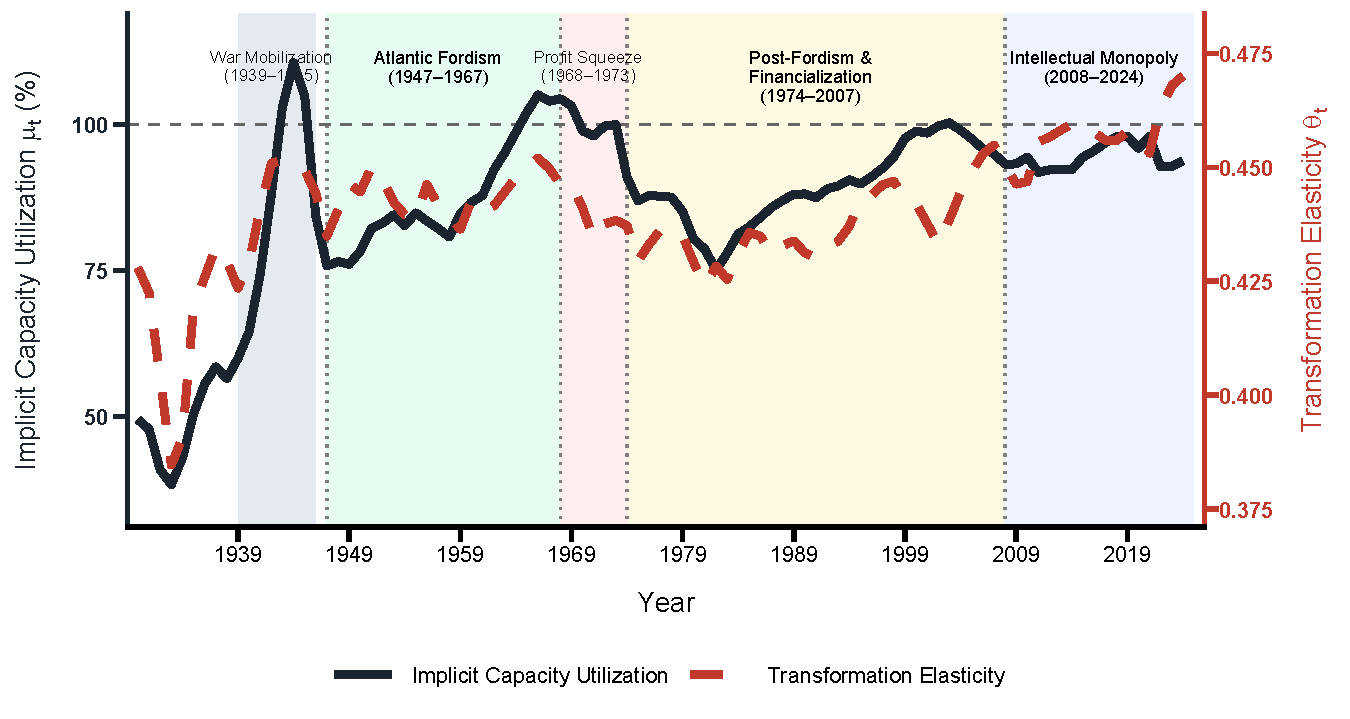
\includegraphics[width=\textwidth]{figures/US_fig4312_dual_theta_mu_enhanced.pdf}
		\caption{Implicit capacity utilization ($\mu_t$, left axis)
			and transformation elasticity ($\theta_t$, right axis).}
		\label{fig:us_fig4312_dual}
	\end{subfigure}
	
	% Vertical space between the two plots
	\vspace{1.5cm}
	
	% Bottom Subfigure
	\begin{subfigure}[b]{0.95\textwidth}
		\centering
		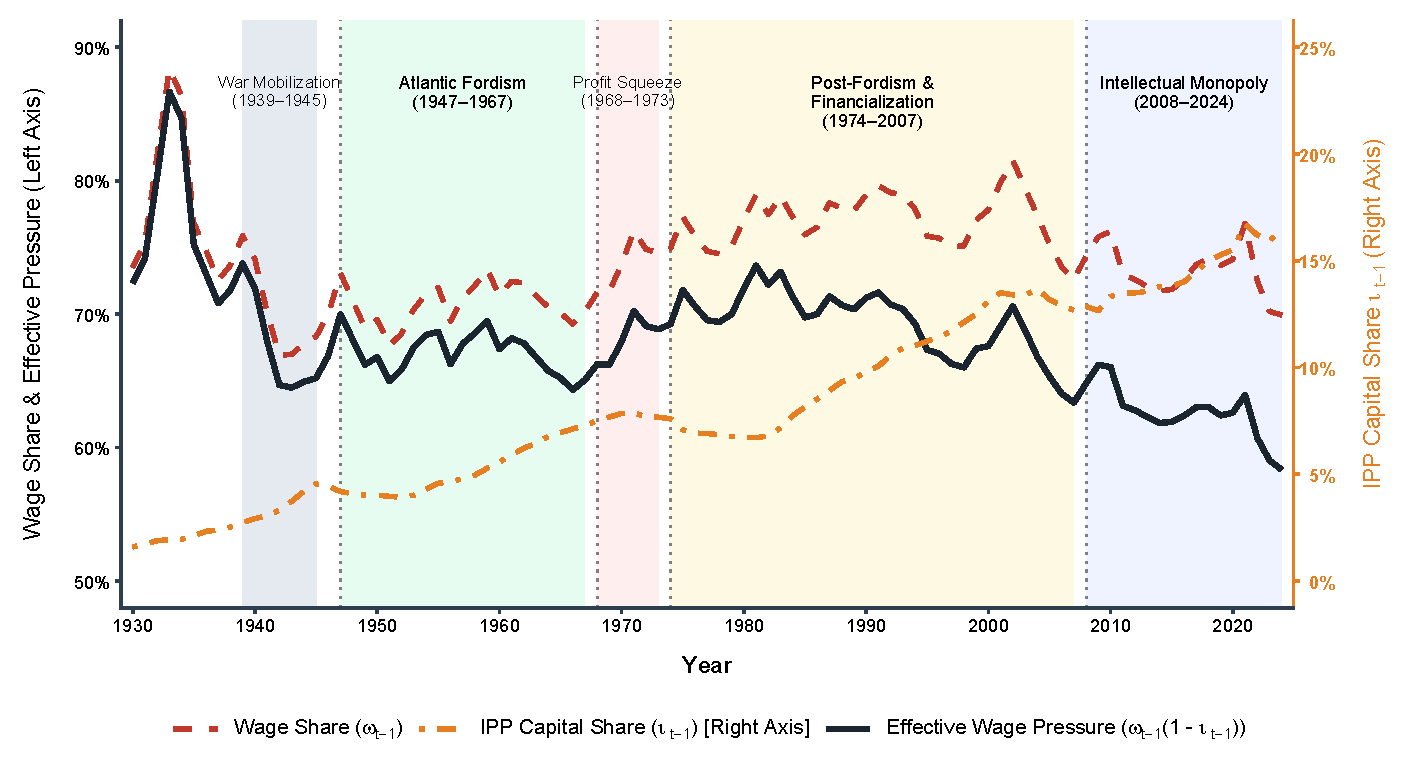
\includegraphics[width=\textwidth]{figures/US_fig4313_dual_axis_subregimes.pdf}
		\caption{Wage share ($\omega_{t-1}$), IPP capital share
			($\iota_{t-1}$, right axis), and effective wage pressure
			($\omega_{t-1}(1-\iota_{t-1})$).}
		\label{fig:us_fig4313_triplet}
	\end{subfigure}
\end{figure}


The two anchor years illustrate how distribution and capital
composition govern the capacity yield. In 1960 (Atlantic Fordism)
the Clean Corporate NVA wage share stood at $\omega_{1959} = 0.72$
while the IPP capital share was negligible
($\iota_{1959} = 0.03$). Effective wage pressure was
$0.72 \times (1 - 0.03) = 0.698$, yielding
$\theta_{1960} = 0.58 - 0.30 \times 0.698 = 0.371$: high wage
pressure forced Okishio-type defensive mechanization, depressing the
marginal capacity yield per dollar of physical capital advanced. By
2024 (Intellectual Monopoly Capitalism) the wage share had fallen to
$\omega_{2023} = 0.70$ while the IPP capital share had risen to
$\iota_{2023} = 0.28$. The intangible diversion reduced effective
wage pressure to $0.70 \times (1 - 0.28) = 0.504$, raising the
transformation elasticity to
$\theta_{2024} = 0.58 - 0.30 \times 0.504 = 0.429$.

\Cref{fig:us_capacity_dynamics_panel} distinguishes five historical
sub-regimes:
\begin{enumerate}
	\item \textbf{War Mobilization (1939--1945).} State-directed
	military planning pushed production past practical capacity
	limits, driving utilization to its historical peak
	($\mu_{1944} = 111.4\%$); wartime retooling raised the
	transformation elasticity to $\theta_t \approx 0.455$.
	\item \textbf{Atlantic Fordism (1947--1967).} High wage shares
	($\omega_{t-1} \approx 0.70$--$0.73$) and minimal intangible
	capital ($\iota_{t-1} < 0.05$) transmitted labor-cost
	pressure directly into mechanization. Potential capacity
	growth was absorbed by wage-led effective demand, holding
	utilization in a stable band
	($\mu_t \approx 85\%$--$105\%$) that crossed $100\%$
	during the mid-1960s expansion.
	\item \textbf{Profit Squeeze (1968--1973).} Distributional
	conflict compressed profit margins and induced defensive
	capital-deepening driven by unit-cost containment rather
	than expansion. The transformation elasticity fell to
	$\theta_{1972} = 0.418$; utilization collapsed to
	$\mu_{1975} = 76.2\%$ and reached its trough
	($\mu_{1982} = 74.1\%$) during the Volcker disinflation.
	\item \textbf{Post-Fordism and Financialization (1974--2007).}
	Organized-labor concessions lowered wage shares while
	investment shifted toward software and patent enclosures
	($\iota_{t-1} > 0.15$), diverting surplus away from labor
	substitution: effective wage pressure fell from $0.72$ in
	1974 to $0.66$ in 1997. The elasticity rose from $0.418$
	to $0.450$, yet utilization never re-anchored to its Fordist
	peak, remaining below $95\%$ outside transient credit-fueled
	expansions.
	\item \textbf{Intellectual Monopoly Capitalism (2008--2024).}
	After the Great Financial Crisis, intangible capital exceeded
	$28\%$ of total fixed capital. The IPP expansion pulled
	effective wage pressure down to $0.504$ in 2024 and raised
	the transformation elasticity toward its upper historical
	range ($\theta_{2024} = 0.429$--$0.470$), while wage
	suppression restricted aggregate realization, leaving
	utilization chronically below full capacity
	($\mu_{2024} = 93.8\%$).
\end{enumerate}

The reconstruction present empirical evidence suports that the long-run horizon does not yield a classical closure ($\mu^* = 100\%$), 
but an unbalanced growth one $\theta^* \neq 1 $from where systemic desiquilibrium arises through different patterns across distinct historical regimes.  
While the Fordist accumulation regime through its commitment to full employment implemented policies oriented to sustain aggregate demand and avoid productive capacities to remain idle, during post-Fordism the expansion of productive capacity ($\theta_t \uparrow$) has decoupled from realization ($\mu_t<1)$, causing persistent idle capacities as an institutional feature.


\subsection{Empirical Estimates Under a Heterogeneous Capital Specification}
\label{sec:432:specB_results}

\subsubsection{Econometric Specifiation of Mechanization Bias and Heterogenous Capital}
Specification A treats aggregate core capital $k_{\text{cap},t} = \log(K_{\text{ME},t} + K_{\text{NRC},t})$ as a single regressor. This collapses the physical structure of the workplace into a scalar, obscuring whether wage pressure operates through the \emph{level} of capital or through its \emph{composition}---the relative weight of machinery and equipment ($K^{\text{ME}}$) versus nonresidential structures ($K^{\text{NRC}}$). Specification B decomposes the aggregate into two components: a structural base ($k^{\text{NRC}}_t = \log K^{\text{NRC}}_t$) and the capital composition ratio ($\kappa_t = k^{\text{ME}}_t - k^{\text{NRC}}_t$), which measures the mechanization gap between equipment and structures in log-levels. The disaggregated cointegrating equation takes the form:
\begin{equation}
	y_t = \alpha + \theta_{\text{NRC}}\, k^{\text{NRC}}_t + \theta_\kappa\, \kappa_t + \theta_{\omega\kappa}\, \xi^{\omega\kappa}_t + \theta_{\kappa p}\, \xi^{p\kappa}_t + \boldsymbol{\gamma}' \mathbf{D}_t + u_t,
	\label{eq:432:specB_model}
\end{equation}
where $\xi^{\omega\kappa}_t$ denotes the FWL-orthogonalized effective wage--mechanization interaction and $\xi^{p\kappa}_t$ denotes the FWL-orthogonalized relative price--mechanization interaction. Both interaction terms are residualized against the two base capital regressors ($k^{\text{NRC}}_t, \kappa_t$) and deterministic step shifts ($\mathbf{D}_t$) prior to estimation. The effective wage interaction under Set~2 is $\xi^{\omega\kappa}_t = \omega_{t-1}(1-\iota_{t-1}) \times \kappa_t$; the relative price interaction is $\xi^{p\kappa}_t = p^{\kappa}_t \times \kappa_t$, where $p^{\kappa}_t$ denotes the relative asset price ratio. Non-standard fixed-$b$ critical values are generated from a dedicated 100,000-pass Monte Carlo simulation engine that replicates the exact Specification~B integration geometry---five independent $I(1)$ stochast
ic trends, two simultaneous $I(1) \times I(1)$ interaction products, and joint FWL orthogonalization---matching the empirical sample sizes ($T = 94$ and $T = 77$).

\paragraph{Economic intuition of the decomposition.}
The parameter $\theta_{\text{NRC}}$ captures the long-run capacity yield of structures---factories, warehouses, commercial buildings---which embody extensive accumulation: expanding the physical envelope within which production occurs. The parameter $\theta_\kappa$ captures the additional capacity yield of machinery and equipment \emph{above and beyond} what structures deliver. A positive $\theta_\kappa$ means that a wider mechanization gap---more equipment per dollar of structures---raises productive capacity independently of the total capital stock. The interaction $\theta_{\omega\kappa}$ asks whether effective wage pressure conditions this compositional margin. Under the Okishio-induced mechanization mechanism, rising wages force firms to substitute equipment for labor on the shop floor. If the resulting machinery expansion is defensive---driven by unit-cost containment rather than autonomous technical expansion---it raises the equipment-to-structures ratio without proportionally expanding output capacity, yielding $\theta_{\omega\kappa} < 0$.

\paragraph{Standard wage interactions fail at the intensive margin.}
Tables~\ref{tab:specB_set1_gva_app} and \ref{tab:specB_set1_nva_app} in Appendix~\ref{app:specB_full_results} present the estimation results using the unadjusted wage share across all 24 specifications. The structural base elasticity $\hat{\theta}_{\text{NRC}}$ remains stable and highly significant ($0.47$--$0.61$, $p < 0.01$), confirming that nonresidential structures anchor the cointegrating relationship regardless of wage measure or break treatment. The standalone mechanization gap $\hat{\theta}_\kappa$ is positive in nearly all models ($0.34$--$1.11$), indicating that equipment contributes to capacity above structures. The wage--mechanization interaction $\hat{\theta}_{\omega\kappa}$, however, fails to achieve statistical significance in any $T = 94$ model, with point estimates ranging from $-4.89$ ($t = -1.58$) to $+7.95$ ($t = 1.33$). The standard wage interaction fails at the intensive margin for the same reason it fails at the aggregate level in Specification~A: unadjusted wage shares conflate supervisory overhead with productive variable capital and ignore the post-Fordist diversion of investment toward intellectual property products.

\paragraph{Effective wage pressure and defensive mechanization at the intensive margin.}
Table~\ref{tab:specB_set2_nva_main} presents the main estimates using the effective wage pressure measure for the NVA basis. When effective wage pressure is scaled by $(1-\iota_{t-1})$ and interacted with the mechanization gap $\kappa_t$, the wage--mechanization interaction $\hat{\theta}_{\omega\kappa}$ is negative and statistically significant across all eight models. In the preferred Clean Corporate Tier~1 NVA specification with Bai-Perron step shifts (Column~4), $\hat{\theta}_{\omega\kappa} = -7.93$ ($SE = 2.96$, $p < 0.05$), with a structural base elasticity of $\hat{\theta}_{\text{NRC}} = 0.60$ ($SE = 0.08$, $p < 0.01$) and a standalone mechanization gap of $\hat{\theta}_\kappa = 0.39$ ($SE = 0.29$). In the Shaikh-Tonak Tier~2 NVA specification without breaks (Column~7), the interaction strengthens to $\hat{\theta}_{\omega\kappa} = -17.05$ ($SE = 2.34$, $p < 0.01$), with $\hat{\theta}_{\text{NRC}} = 0.54$ ($SE = 0.01$) and $\hat{\theta}_\kappa = 0.33$ ($SE = 0.06$, $p < 0.01$). The Clean Corporate Tier~2 NVA models (Columns~5--6) yield $\hat{\theta}_{\omega\kappa} = -14.97$ ($SE = 2.01$, $p < 0.01$), showing the tightest standard errors in the table.

The negative sign of $\hat{\theta}_{\omega\kappa}$ provides direct evidence of defensive mechanization operating at the \emph{intensive margin} of capital composition. Specification~A established that effective wage pressure depresses the aggregate capacity yield of total capital ($\hat{\theta}_1 = -0.30$). Specification~B isolates the channel: wage pressure forces firms to widen the mechanization gap---substituting equipment for structures on the shop floor---but the capacity yield of that compositional shift is negative. The firm accumulates more machinery per dollar of structures, yet productive capacity does not expand proportionally, because the substitution is driven by cost containment rather than by genuine technical complementarity between new equipment and existing plant.\footnote{The apparent difference in magnitude between Specification~A ($\hat{\theta}_1 \approx -0.30$) and Specification~B ($\hat{\theta}_{\omega\kappa} \approx -7.93$ to $-17.05$) reflects regressor scaling, not economic inconsistency. In Specification~A, $\theta_1$ multiplies $\omega_{t-1}(1-\iota_{t-1}) \times k_{\text{cap},t}$, where aggregate capital $k_{\text{cap},t} \approx 16$--$17$ in log-levels. In Specification~B, $\theta_{\omega\kappa}$ multiplies $\omega_{t-1}(1-\iota_{t-1}) \times \kappa_t$, where the mechanization gap $\kappa_t = k^{\text{ME}}_t - k^{\text{NRC}}_t \approx 0.3$--$0.8$. The total marginal effect (coefficient $\times$ regressor scale) is comparable across both specifications.}

\paragraph{Relative price interactions.}
The relative asset price interaction $\hat{\theta}_{\kappa p}$ is generally small and statistically insignificant. In the NFC Baseline and Clean Corporate Tier~1 models (Columns~1--4), it is statistically indistinguishable from zero. In the Shaikh-Tonak Tier~2 specification (Columns~7--8), $\hat{\theta}_{\kappa p} = -0.79$ ($SE = 0.32$, $p < 0.05$), suggesting that when equipment becomes relatively more expensive, the capacity yield of the mechanization gap declines. However, this result is fragile and does not hold across wage share measures. The Okishio mechanism operates through distributional conflict over newly created value, not through relative asset prices.

\paragraph{Cointegration inference.}
The effective wage models show strong evidence of cointegration. The Shin LM test never rejects the null of cointegration ($C_{\text{Shin}} \le 0.03$, $p > 0.10$), and the Vogelsang-Wagner Type~2 Wald statistic remains well below critical thresholds ($S_{\text{Type~2}} \le 15.37$). The Engle-Granger residual ADF test rejects the null of no cointegration at the 5\% level in every break-adjusted model: $t_{\text{ADF}} = -4.58$ (Column~2), $-4.60$ (Column~4), $-4.71$ (Column~7), and $-4.57$ (Column~8). Without step shifts, the ADF test rejects at the 10\% level across all $T = 94$ models ($t_{\text{ADF}} \le -4.33$) and at the 5\% level for the $T = 76$ Shaikh-Tonak Tier~2 model ($t_{\text{ADF}} = -4.71$, Column~7). The full cointegration triad---Shin, Vogelsang-Wagner, and ADF---confirms that the disaggregated capital composition, real output, and effective wage pressure form a stable long-run relationship.

\paragraph{Robustness.}
Including Bai-Perron step shifts absorbs historical level discontinuities, but leaves the sign and significance of the wage--mechanization interaction unchanged. In the Clean Corporate Tier~1 NVA model, controlling for breaks at 1944, 1977, and 2001 sharpens the ADF rejection from $-4.34$ ($p < 0.10$) to $-4.60$ ($p < 0.05$) while reducing the Vogelsang-Wagner statistic from $15.37$ to $6.37$. The wage interaction $\hat{\theta}_{\omega\kappa}$ moves from $-11.08$ (Column~3) to $-7.93$ (Column~4). This modest attenuation indicates that the step dummies absorb part of the interaction's raw variance. The interaction remains negative and significant at the 5\% level, confirming that the compositional conditioning channel survives institutional break controls.

The structural base elasticity $\hat{\theta}_{\text{NRC}}$ falls consistently within the $0.51$--$0.61$ band across wage share measures, closely tracking the aggregate $\hat{\theta}_0 = 0.58$ from Specification~A. This implies the capacity yield of structures is a stable parameter of U.S.\ capital accumulation. The wage interaction $\hat{\theta}_{\omega\kappa}$ grows larger in absolute value as we remove supervisory overhead from the wage share: from $-10.13$ in the NFC Baseline (Column~2) to $-7.93$ in Clean Corporate Tier~1 (Column~4) to $-16.76$ in Shaikh-Tonak Tier~2 (Column~8). Removing managerial salaries isolates the productive variable capital driving the firm's cost-minimization decision, which sharpens the defensive mechanization effect.

\begin{table}[h!]
	\centering
	\caption{Specification B, Set 2: Effective Wage Interaction (NVA Basis)}
	\label{tab:specB_set2_nva_main}
	\small
	\begin{tabular}{p{3.0cm}p{1.25cm}p{1.25cm}p{1.25cm}p{1.25cm}p{1.5cm}p{1.5cm}p{1.5cm}p{1.5cm}}
		\toprule
		& \multicolumn{2}{c}{NFC NVA Baseline} & \multicolumn{2}{c}{Clean Corp Tier 1} & \multicolumn{2}{c}{Clean Corp Tier 2} & \multicolumn{2}{c}{ST Tier 2 NVA} \\
		\cmidrule(lr){2-3} \cmidrule(lr){4-5} \cmidrule(lr){6-7} \cmidrule(lr){8-9}
		& (1) & (2) & (3) & (4) & (5) & (6) & (7) & (8) \\
		\midrule
		$\hat{\theta}_{\text{NRC}}$  (Structures $k^{\text{NRC}}$) & 0.61$^{***}$ & 0.58$^{***}$ & 0.60$^{***}$ & 0.60$^{***}$ & 0.54$^{***}$ & 0.54$^{***}$ & 0.54$^{***}$ & 0.51$^{***}$ \\
		& (0.02) & (0.08) & (0.02) & (0.08) & (0.01) & (0.01) & (0.01) & (0.01) \\
		$\hat{\theta}_{\kappa}$ (Mechanization Gap $\kappa$) & 0.32$^{*}$ & 0.39 & 0.32$^{*}$ & 0.39 & 0.31$^{***}$ & 0.31$^{***}$ & 0.33$^{***}$ & 0.06 \\
		& (0.13) & (0.29) & (0.13) & (0.29) & (0.06) & (0.06) & (0.06) & (0.09) \\
		$\hat{\theta}_{\omega\kappa}$ (Wage Interaction) & -12.77$^{**}$ & -10.13$^{**}$ & -11.08$^{**}$ & -7.93$^{**}$ & -14.97$^{***}$ & -14.97$^{***}$ & -17.05$^{***}$ & -16.76$^{***}$ \\
		& (3.81) & (3.43) & (3.48) & (2.96) & (2.01) & (2.01) & (2.34) & (2.55) \\
		$\hat{\theta}_{\kappa p}$ (Price Interaction) & 0.18 & 0.92 & 0.69 & 1.41$^{*}$ & -0.31 & -0.31 & -0.79$^{**}$ & -0.71$^{**}$ \\
		& (0.51) & (0.69) & (0.63) & (0.75) & (0.33) & (0.33) & (0.32) & (0.31) \\
		\midrule
		Step Shifts ($D_{T_b}^{\text{step}}$) & No & Yes & No & Yes & No & Yes & No & Yes \\
		$C_{\text{Shin}}$ [$H_0$: coint.] & 0.03 & 0.02 & 0.03 & 0.03 & 0.02 & 0.02 & 0.02 & 0.02 \\
		$S_{\text{Type 2}}$ [$H_0$: coint.] & 14.97 & 5.93 & 15.37 & 6.37 & 8.96 & 8.96 & 10.28 & 8.70 \\
		$t_{\text{ADF}}$ [$H_0$: no coint.] & -4.33$^{*}$ & -4.58$^{**}$ & -4.34$^{*}$ & -4.60$^{**}$ & -4.24$^{*}$ & -4.24$^{*}$ & -4.71$^{**}$ & -4.57$^{**}$ \\
		Bandwidth ratio $b$ & 0.185 & 0.173 & 0.193 & 0.181 & 0.208 & 0.208 & 0.208 & 0.208 \\
		Sample Size $T$ & 94 & 94 & 94 & 94 & 76 & 76 & 76 & 76 \\
		\bottomrule
	\end{tabular}
	\begin{minipage}{\textwidth}
		\scriptsize
		\textit{Notes:} Dependent variable: $y_t^{\text{NFC}}$ (log NFC real GVA). Estimated via Cointegrating Multivariate Polynomial Regression (CMPR) IM-OLS \citep{VogelsangWagner2024}. Step Shifts "No": no structural break dummies; "Yes": Bai-Perron step dummies included. All interaction terms are FWL-orthogonalized against base capital regressors ($k^{\text{NRC}}_t, \kappa_t$) and step dummies. The effective wage interaction is $\xi^\omega_t = \omega_{t-1}(1-\iota_{t-1}) \times \kappa_t$, where $\kappa_t = k^{\text{ME}}_t - k^{\text{NRC}}_t$ is the capital composition ratio (mechanization gap) and $\iota_{t-1}$ is the lagged IPP share of capital. Significance: $^*p<0.10$, $^{**}p<0.05$, $^{***}p<0.01$. Stars for coefficient rows and cointegration tests are derived from a 100,000-pass Monte Carlo simulation suite mapping the exact DGP variant and fixed-$b$ Wald tables. Standard errors in parentheses.
	\end{minipage}
\end{table}


\subsubsection{Transformation Elasticity from Heterogeneous Capital Specification and Capacity Utilization Estimates}

\paragraph{The transformation elasticity along the historical path.}
Having established the structural asset-weighted transformation elasticity $\theta^{\text{SpecB}}_t$ in Equation~\eqref{eq:32:theta_aggregate_structural} (Section~3.2), I evaluate its empirical trajectory using the estimated parameters from the preferred Specification~B model (Clean Corporate Tier~1 NVA, Set~2, Column~4 of Table~\ref{tab:specB_set2_nva_main}). The structural marginal capacity yield of mechanization $MP_{\kappa,t}^{\text{str}} = \beta_\kappa + \theta_{\omega\kappa} C_{\text{index},t} + \theta_{\kappa p} p^\kappa_t$ is driven directly by the state-dependent levels of effective wage pressure ($C_{\text{index},t}$) and relative asset prices ($p^\kappa_t$).\footnote{\textbf{REMINDER}: initial-observation centering ($\theta_\kappa^{\text{str}} = 0.39$) serves as an anchoring convention to identify the baseline dimensionless yield at $t=1931$. \textbf{TASK:} Present this formulation in the methodology 4.2 section or elsewhere.} 

Figure~\ref{fig:specB_candidate1} plots $\theta^{\text{Aggregate}}_t$ against the dynamic Specification~A baseline ($\theta^{\text{SpecA}}_t = 0.58 - 0.30 \cdot C_{\text{index},t}$) and the Harrodian knife-edge threshold ($\theta = 1.00$) under standard structural regime shading.

\begin{figure}[h!]
	\centering
	\caption{Aggregate Transformation Elasticity ($\theta^{\text{Aggregate}}_t$), Specification~B vs.\ Baseline}
	\label{fig:specB_candidate1}
	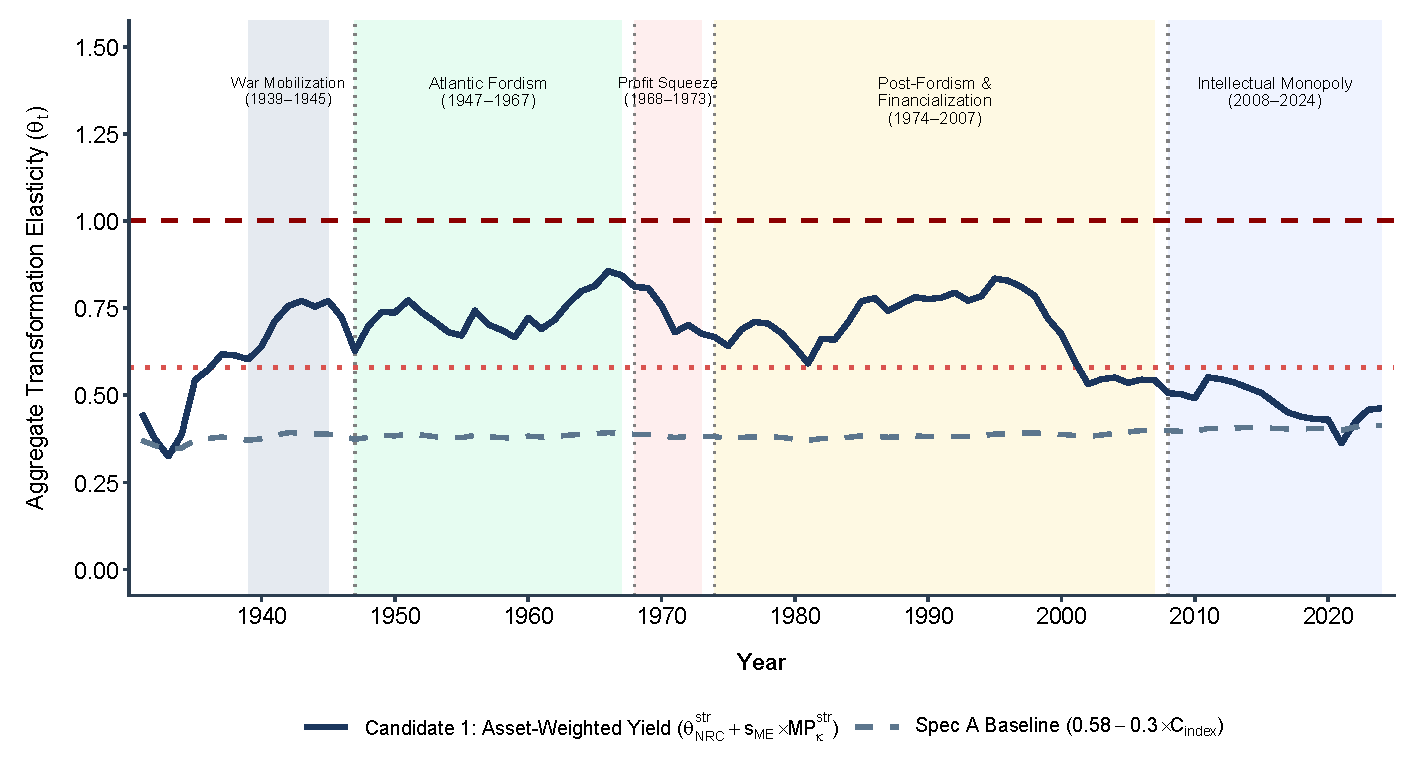
\includegraphics[width=0.95\textwidth]{figures/fig_specB_candidate1_aggregate_elasticity.pdf}
	\begin{tabular}{p{0.88\textwidth}}	
		\footnotesize \textbf{Note:} Aggregate transformation elasticity $\theta^{\text{Aggregate}}_t$ (Navy line) computed according to Equation~\eqref{eq:32:theta_aggregate_structural} using FWL structural parameters from the preferred Specification~B model (Clean Corporate Tier~1 NVA, Set~2, Column~4 of Table~\ref{tab:specB_set2_nva_main}). The Slate Blue line traces the dynamic Specification~A baseline ($\theta^{\text{SpecA}}_t = 0.58 - 0.30 \, C_{\text{index},t}$). The dotted horizontal line at $\theta = 0.58$ marks the constant base from Specification~A. The dashed line at $\theta = 1.00$ marks the Harrodian knife-edge. Background shading indicates structural accumulation regimes. \\
	\end{tabular}
\end{figure}

\textbf{REMINDER 1: The plot should have bigger size font and should plot not only the baseline of the transformation elasticity from the baseline specification but also its dynamic trajectory}

\textbf{REMINDER 2:} $\theta$ \textbf{IN this section requires being defined coherently with the visit to the cambridge critique on aggregation of heterogeneous capital as in \cref{sec:3:analytical_framework}}


\paragraph{Empirical comparison: Specification~B disciplines the Specification~A baseline.}
Figure~\ref{fig:specB_candidate1} delivers two core empirical findings. First, the structural elasticity $\theta^{\text{SpecB}}_t$ closely tracks the dynamic Specification~A path but operates within a narrower, disciplined band---$[0.32, 0.86]$ versus $[0.37, 0.75]$. The two paths move together because both capture the same underlying macroeconomic force: effective wage pressure depresses the marginal capacity yield of capital across both specifications, and the estimated base elasticity of structures ($\hat{\theta}_{\text{NRC}} \approx 0.60$) matches Specification~A's aggregate base ($\hat{\theta}_0 = 0.58$). Second, the Specification~B trajectory remains strictly below the Harrodian knife-edge ($\theta < 1$) across the entire 1931--2024 sample, confirming that aggregate capacity formation in the U.S.\ economy operates permanently within the sub-Harrodian stability regime.

The disaggregated capital structure explains what Specification~A's aggregate elasticity averages over. During the Fordist era ($C_{\text{index},t} > 0.65$), high effective wage pressure drove negative marginal mechanization yields ($MP_{\kappa,t}^{\text{str}} < 0$). Firms substituted equipment for labor to contain unit labor costs, but because this expansion was defensive rather than technically autonomous, it depressed the aggregate capacity yield of total capital. In the Neoliberal period ($C_{\text{index},t} < 0.50$), declining wage pressure restored $MP_{\kappa,t}^{\text{str}}$ to positive territory, pulling $\theta^{\text{Aggregate}}_t$ back toward the structural base. Specification~A collapses this compositional mechanism into a scalar interaction ($\hat{\theta}_1 = -0.30$); Specification~B opens the intensive margin and confirms the Okishio mechanism empirically.

\begin{figure}[h!]
	\centering
	\caption{Empirical Accumulation Path Derivatives ($dk^{\text{ME}} / dk^{\text{NRC}}$ and $d\kappa / dk^{\text{NRC}}$)}
	\label{fig:specB_dkappa_dknrc_slope}
	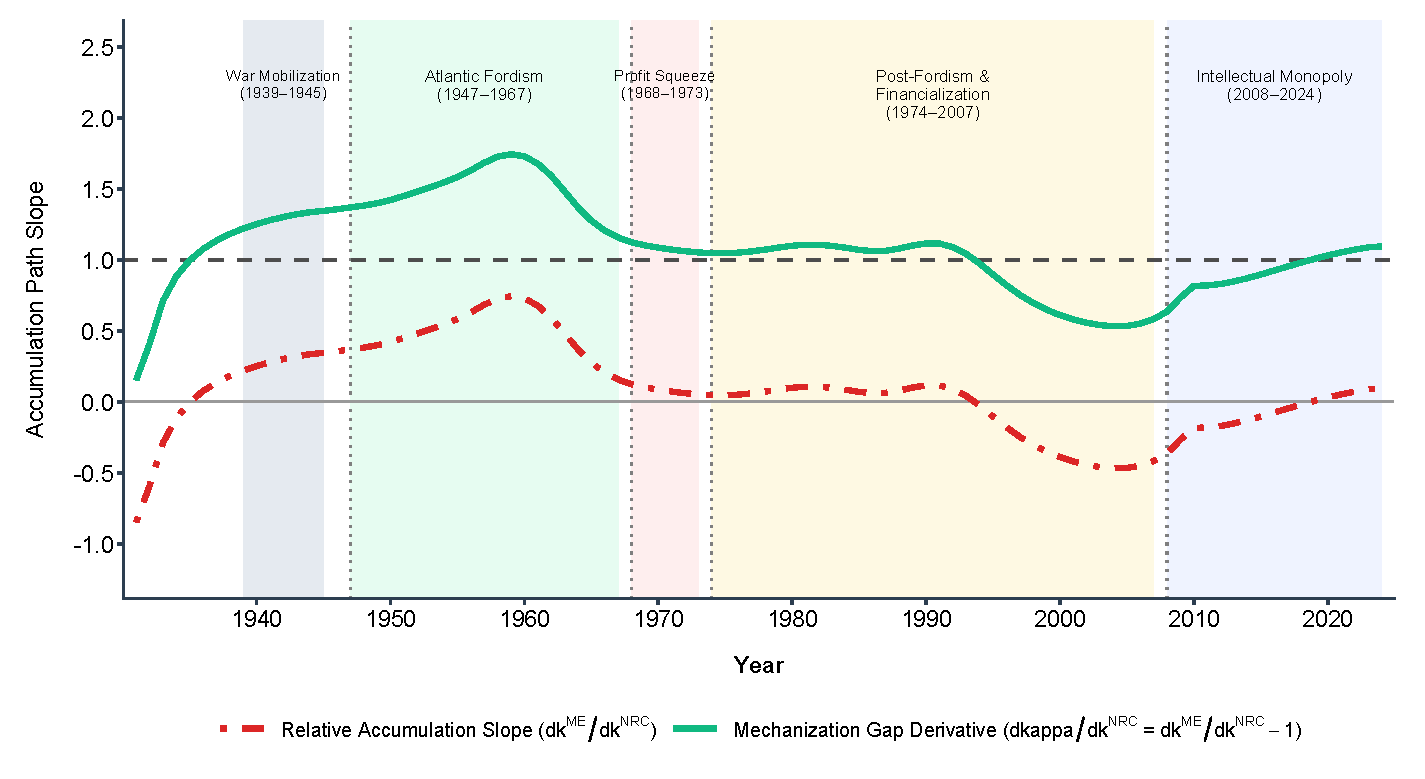
\includegraphics[width=0.88\textwidth]{figures/fig_specB_dkappa_dknrc_slope.pdf}
	\begin{tabular}{p{0.88\textwidth}}
		\footnotesize \textbf{Note:} Empirical accumulation path derivatives estimated via non-parametric LOESS time-domain chain rule ($\text{span} = 0.35$). The green solid line measures the relative accumulation slope $dk^{\text{ME}}_t / dk^{\text{NRC}}_t$. The red dot-dashed line measures the mechanization gap derivative $d\kappa_t / dk^{\text{NRC}}_t = (dk^{\text{ME}}_t / dk^{\text{NRC}}_t) - 1$. The horizontal dashed line at $1.00$ indicates balanced expansion where equipment and structures grow at identical rates. \\
	\end{tabular}
\end{figure}

\paragraph{Empirical failure of the conventional Divisia derivative path.}
Figure~\ref{fig:specB_dkappa_dknrc_slope} illustrates why the empirical total-derivative path $\theta^{\text{Aggregate}}_{\text{total},t}$ (Equation~\eqref{eq:32:theta_aggregate}) fails in practice. In the mid-1990s, corporate accumulation shifted away from physical machinery toward intellectual property products and financial assets, causing physical equipment growth to slow relative to structures ($dk^{\text{ME}}_t / dk^{\text{NRC}}_t < 1.00$). As $d\kappa_t / dk^{\text{NRC}}_t$ crossed zero, the Divisia denominator in Equation~\eqref{eq:32:theta_aggregate} approached zero, sending the raw total-derivative elasticity to spurious infinite spikes. As established in Section~3.2, this instability reflects the theoretical pathology of differentiating a value aggregate under structural accumulation shifts. The structural asset-weighted elasticity $\theta^{\text{Aggregate}}_t$ in Equation~\eqref{eq:32:theta_aggregate_structural} purges these Divisia singularities, yielding a continuous, empirically well-behaved trajectory.


\paragraph{Driving Forces} The inclusion of heterogeneous capital reveals a structural paradox in the post-war US economy: while the relative cheapening of machinery drove a massive shift in the physical composition of capital, the capacity-generating power of this mechanization was severely degraded by the distributive conflicts of the late 1960s and early 1970s. Figure \ref{fig:US_fig432_dual_theta_mu_specB} plots the implicit capacity utilization rate ($\mu_t$) alongside the asset-weighted aggregate transformation elasticity ($\theta_t^{\text{Spec}}$. Unlike the static baseline elasticity of Specification A, the transformation elasticity here is not solely driven by the evolving mix of machinery and structures, and the macroeconomic environment mediating their installation. As the physical accumulation of machinery and equipment accelerated relative to nonresidential structures, the aggregate transformation elasticity collapsed, severing the Harrodian link between accumulation and potential output. This structural degradation is not an artifact of index-number aggregation but the direct result of shifting marginal capacity yields. To unpack the mechanics of this collapse, Figure \ref{fig:US_fig4323_dual_axis_driving_forces} illustrates the two primary institutional driving forces behind this choice of technique: the secular decline in relative asset prices ($p_t^{\kappa} = P_t^{\text{ME}}/P_t^{\text{NRC}}$) and the episodic spikes in effective distributive pressure ($C_t = \omega_{t-1}(1-\iota_{t-1})$).

Consider a given period during the Golden Age of American Capitalism (e.g., the 1950s) where the structural yield of nonresidential structures is $\theta_{\text{NRC}}^{\text{str}} = 0.60$ and the equipment share is $s_{\text{ME}} = 0.30$. Under a stable distributive environment, if the marginal capacity yield of mechanization is $MP_{\kappa} = 0.40$, the transformation elasticity yields an order of magnitude around $0.72$ ($\theta^{\text{SpecB}} = 0.60 + 0.30 \times 0.40$). However, as the post-war era progressed, machinery became structurally cheaper, as can be appreciated on the downswing tendency of $p_t^{\kappa}$ in Figure \ref{fig:US_fig4323_dual_axis_driving_forces}, pushing the physical equipment share up toward $0.50$. Likewise, the Profit Squeeze (1968--1973) produced a sharp spike in effective distributive pressure ($C_t$). Because the interaction term $\theta_{\omega\kappa}$ is negative, this heightened wage pressure pushing firms into a defensive tactical choice of technique, increasing their efforts for capital-using labor-saving mechanization, i.e. Marx-biased technical change \citep{Basu2022}. Consequently, the marginal capacity yield of this machinery dropped significantly (e.g., down to $MP_{\kappa} = 0.20$). Thus, in the post-Fordist era, the aggregate elasticity fell to $0.70$ ($\theta^{\text{SpecB}} = 0.60 + 0.50 \times 0.20$). Even though the physical share of machinery increased by 20 percentage points due to relative cheapening, the capacity-generating power of that machinery collapsed under the weight of defensive investment strategies induced by decreasing profitability. This mechanism explicitly limits accumulation thorugh stagnation tendencies towards over-accumulation due firms over-shooting their investments biased towards mechanization not to expand capacity, but to replace increasingly expensive labor, resulting into an over-accumulation regime crisis due the decreasing returns to mechanization and increasingly harder to transform capital accumulation to productive capacities within the politcal economy of full employment with intense labor militancy \cite{Kalecki1943}. 


\begin{figure}[H]
	\centering
	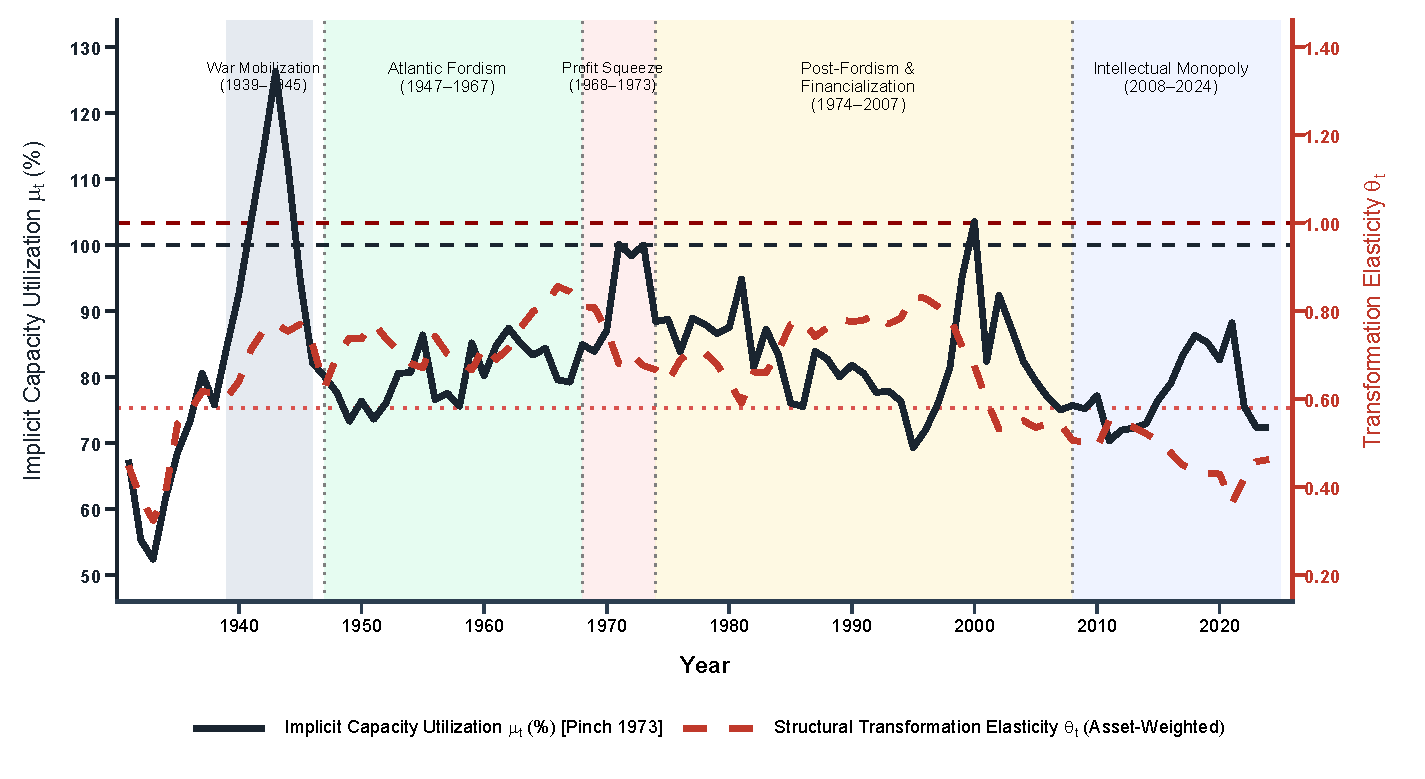
\includegraphics[width=\textwidth]{figures/US_fig432_dual_theta_mu_specB.pdf}
	\caption{Implicit Capacity Utilization ($\mu_t$) and Asset-Weighted Transformation Elasticity ($\theta_t^{\text{Aggregate}}$)}
	\label{fig:US_fig432_dual_theta_mu_specB}
	
	\vspace{0.2cm}
	\parbox{\textwidth}{\footnotesize \textit{Note:} The figure plots the reconstructed capacity utilization rate anchored at the 1973 pinch year alongside the dynamic aggregate transformation elasticity derived from Specification B. The Harrodian knife-edge ($\theta=1.00$) and the Specification A baseline ($\theta=0.58$) are provided as reference lines.}
\end{figure}
\begin{figure}[H]
	\centering
	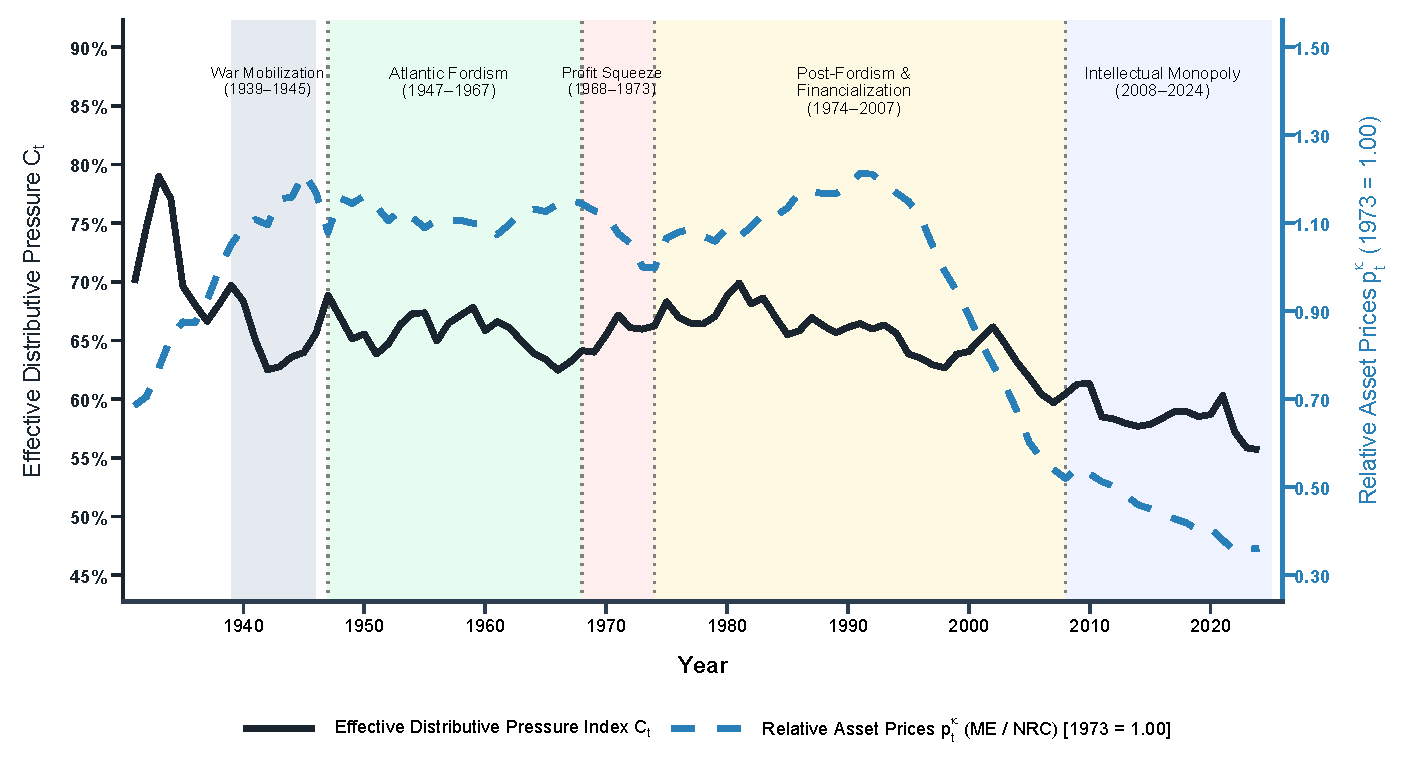
\includegraphics[width=\textwidth]{figures/US_fig4323_dual_axis_driving_forces.pdf}
	\caption{Effective Distributive Pressure ($C_t$) and Relative Asset Prices ($p_t^{\kappa}$)}
	\label{fig:US_fig4323_dual_axis_driving_forces}
	
	\vspace{0.2cm}
	\parbox{\textwidth}{\footnotesize \textit{Note:} The figure illustrates the institutional driving forces behind the choice of technique. The left axis tracks the effective distributive pressure to mechanize ($C_t$), while the right axis tracks the relative price of machinery and equipment to nonresidential structures ($p_t^{\kappa}$, indexed to $1973 = 1.00$).}
\end{figure}


%%%%%%%%%%%%%%%%%%%%%%%%%%%%%%%%%%%%%%%%%%%%%%%%%
%%%%% 4.5. Chile Results 
%%%%%%%%%%%%%%%%%%%%%%%%%%%%%%%%%%%%%%%%%%%%%%%%%
\subsection{Chilean Empirical Evidence: The Peripheral and External Constraints}
\label{sec:44:chile_results}

\subsubsection{Econometric Strategy: Threshold Cointegrating Multivariate Polynomial Regression}
\label{sec:441:chile_strategy}

In core economies, capital accumulation converts into productive capacity through domestic technical choice. Rising wages induce capitalists to substitute labor with machinery, expanding capacity unless surplus is diverted into unproductive accumulation \citep{Rotta2018}. In peripheral economies like Chile, this mechanism depends on international liquidity. Because capital equipment ($K_t^{\text{ME}}$) cannot be produced domestically, labor-saving technical change requires imported machinery. When foreign-exchange reserves collapse, peripheral firms hit a structural bottleneck. Rather than adjusting smoothly through domestic prices, the capacity-generating effect of capital accumulation breaks down: wage pressure cannot induce mechanization because firms cannot acquire the foreign exchange needed to import machinery.

To evaluate this state-dependent breakdown, we estimate a Cointegrating Multivariate Polynomial Regression (CMPR) using Integrated Modified OLS (IM-OLS) \citep{VogelsangWagner2024} with an endogenously identified threshold regime. The estimating equation models log real GDP ($y_t$) as a cointegrating function of non-residential construction ($k_t^{\text{NR}}$), the capital composition gap ($\kappa_t$), distributional conflict ($\text{dist}_{t-1}$), the state-dependent external constraint ($D_t^{\gamma}$), and relative price shocks ($\tilde{p}_t^\perp$):

\begin{equation}
	y_t = \alpha + \theta_1 k_t^{\text{NR}} + \theta_2 \kappa_t + \theta_3 (\text{dist}_{t-1} \cdot \kappa_t) + \theta_4 (\kappa_t \cdot D_t^{\gamma}) + \theta_5 (\text{dist}_{t-1} \cdot \kappa_t \cdot D_t^{\gamma}) + \beta_p \tilde{p}_t^\perp + u_t
\end{equation}

where $y_t$ is log real GDP (2003 CLP); $k_t^{\text{NR}} = \ln K_t^{\text{NR}}$ is the log net stock of non-residential structures; $\kappa_t = \ln(K_t^{\text{ME}} / K_t^{\text{NR}})$ is the capital composition gap between intensive machinery and extensive structures; $\text{dist}_{t-1}$ is the lagged distributive variable, evaluated across four permutations: net wage share ($\omega_{t-1}^{\text{net}}$), gross wage share ($\omega_{t-1}^{\text{gross}}$), net rate of exploitation ($e_{t-1}^{\text{net}}$), and gross rate of exploitation ($e_{t-1}^{\text{gross}}$); $D_t^{\gamma} = \mathbb{I}(Z_t \le \gamma)$ is a binary regime indicator equal to 1 when the composite balance-of-payments index ($Z_t$) falls below threshold $\gamma$; $\tilde{p}_t^\perp$ is the standardized relative capital price, orthogonalized against physical capital stocks via Frisch-Waugh-Lovell (FWL) regression; and $u_t$ is a stationary $I(0)$ error.

The partial derivative of output $y_t$ with respect to the capital composition gap $\kappa_t$ yields the marginal transformation elasticity $\theta(\text{dist}, D_t)$:

\begin{equation}
	\frac{\partial y_t}{\partial \kappa_t} = \theta_2 + \theta_3 \text{dist}_{t-1} + \theta_4 D_t^{\gamma} + \theta_5 (\text{dist}_{t-1} \cdot D_t^{\gamma})
\end{equation}

The coefficients carry direct political-economy interpretations:
\begin{enumerate}
	\item \textbf{Extensive Construction Elasticity ($\theta_1$)}: Measures capacity generated by non-residential construction.
	\item \textbf{Unconstrained Mechanization Elasticity ($\theta_2$)}: Measures capacity generated by intensive capital composition under normal liquidity ($D_t^{\gamma} = 0$).
	\item \textbf{Domestic Induced Innovation ($\theta_3$)}: Captures wage-led induced technical change under unconstrained liquidity, where worker bargaining power forces capitalists to substitute labor with machinery.
	\item \textbf{Balance-of-Payments Structural Shift ($\theta_4$)}: Measures the direct collapse in mechanization capacity when external constraints bind ($D_t^{\gamma} = 1$).
	\item \textbf{Peripheral Distributional Inversion ($\theta_5$)}: Captures the breakdown in wage-led technical change under foreign-exchange starvation. A negative estimate ($\theta_5 < 0$) demonstrates that when reserves collapse, wage pressure cannot induce mechanization because imported machinery is rationed.
\end{enumerate}

\paragraph{Constructing the Balance-of-Payments Threshold Index ($Z_t$)}
We define the composite balance-of-payments index $Z_t(p)$ as a convex linear combination of two standardized macroeconomic indicators:

\begin{equation}
	Z_t(p) = p \, \tilde{M}_t + (1 - p) \, \tilde{S}_t, \quad p \in [0, 1]
\end{equation}

where $\tilde{S}_t = \text{scale}(F_t / M0_t)$ measures central bank foreign reserves ($F_t = e_t \cdot \text{IR}_t$) relative to base money ($M0_t$) \citep{NievasPiketty2025}, and $\tilde{M}_t = \text{scale}(\text{Imbalance}_t)$ measures the capital-goods import demand imbalance. 

Because the structural weight $p$ and threshold level $\gamma$ are unknown \textit{a priori}, we estimate $(\hat{p}, \hat{\gamma})$ via a joint profile Sum of Squared Residuals (SSR) search:

\begin{equation}
	(\hat{p}, \hat{\gamma}) = \arg\min_{p \in \mathcal{P}, \, \gamma \in \Gamma(p)} \text{SSR}(p, \gamma) = \arg\min_{p \in \mathcal{P}, \, \gamma \in \Gamma(p)} \sum_{t=1}^{T} \hat{u}_t(p, \gamma)^2
\end{equation}

The weighting grid $\mathcal{P} = \{ 0.0, 0.1, 0.2, \dots, 1.0 \}$ steps across the unit interval in increments of 0.1. For each candidate weight $p$, the threshold grid $\Gamma(p)$ evaluates trimmed quantiles $\Gamma(p) = \{ \gamma_q(p) : q \in [0.15, 0.85], \, \Delta q = 0.05 \}$. The global minimizer selects $\hat{p} = 0.2$ ($Z_t = 0.2 \tilde{M}_t + 0.8 \tilde{S}_t$) and $\hat{\gamma} = 0.425$ (or $\hat{\gamma} = 0.379$ in parsimonious specifications), confirming that international reserve cover ($\tilde{S}_t$) dominates the empirical weighting in isolating the structural bottleneck.

\paragraph{Bai-Perron Structural Break Benchmark}
To confirm that $D_t^{\gamma}$ captures a genuine balance-of-payments constraint rather than a deterministic calendar trend, we compare the threshold model against a benchmark specification using \citet{BaiPerron2003} endogenous structural breaks:
\begin{equation}
	y_t = \alpha + \theta_1 k_t^{\text{NR}} + \theta_2 \kappa_t + \theta_3 (\text{dist}_{t-1} \cdot \kappa_t) + \theta_4 (\kappa_t \cdot D_t^{\text{BP}}) + \theta_5 (\text{dist}_{t-1} \cdot \kappa_t \cdot D_t^{\text{BP}}) + \beta_p \tilde{p}_t^\perp + u_t
\end{equation}
where $D_t^{\text{BP}} = \mathbb{I}(t \ge T_b)$. Dynamic search over candidate break dates $T_b \in [0.15 T, 0.85 T]$ identifies two historical break points:
\begin{itemize}
	\item \textbf{Net Distribution ($\omega^{\text{net}}, e^{\text{net}}$)}: Identifies $T_b = 1987$, marking structural consolidation under the Büchi reforms following the 1982 crisis, where wage suppression and export promotion restored financial stability.
	\item \textbf{Gross Distribution ($\omega^{\text{gross}}, e^{\text{gross}}$)}: Identifies $T_b = 1999$, marking the Asian Financial Crisis in Chile, when the Central Bank floated the Chilean peso and abandoned exchange-rate crawling bands.
\end{itemize}
Achieving lower SSR and stronger cointegration statistics under $Z_t \le 0.425$ rules out deterministic calendar trends in favor of true balance-of-payments state dependence.

\paragraph{Relative Price Controls and Asset Deflators}
The relative price control accounts for international purchasing power shifts affecting imported capital equipment. In Chilean historical national accounts, separate long-run deflators for structures ($P_t^{\text{NRC}}$) and machinery ($P_t^{\text{ME}}$) do not exist back to 1940. Capital stock harmonization constructs a single unified investment price deflator ($P_{K,t}$, staged as \texttt{Pk\_2003base}) by splicing historical ClioLab deflators (1940--2010) with official Central Bank of Chile deflators (2003 base year).

We evaluate two complementary proxies:
\begin{enumerate}
	\item \textbf{Baseline Real Exchange Rate Control ($\tilde{p}_t^{\kappa, \text{RER}}$)}: The standardized log Real Effective Exchange Rate ($\ln\text{TCREAL}_t$, rebased to 2003 = 1.0), capturing external purchasing power shocks that alter the domestic price of imported machinery ($K_t^{\text{ME}}$).
	\item \textbf{Robustness Asset-to-Output Ratio ($p_t^{\kappa, P_Y/P_K}$)}: The log ratio of aggregate GDP deflator ($P_{Y,t}$) to unified capital price index ($P_{K,t}$):
	\begin{equation}
		p_t^{\kappa, P_Y/P_K} = \ln\left(\frac{P_{Y,t}}{P_{K,t}}\right)
	\end{equation}
	measuring relative shifts between aggregate output prices and capital goods prices.
\end{enumerate}

To prevent relative price volatility from collinearizing with physical capital stocks ($k_t^{\text{NR}}, \kappa_t$), we extract the orthogonal price component $\tilde{p}_t^\perp$ via a Frisch-Waugh-Lovell (FWL) auxiliary regression prior to estimation:
\begin{equation}
	\tilde{p}_t^{\kappa, \text{RER}} = c_0 + c_1 k_t^{\text{NR}} + c_2 \kappa_t + \tilde{p}_t^\perp
\end{equation}
The residual vector $\tilde{p}_t^\perp$ enters the estimating equation additively. Preliminary grid tests introducing interacted price terms ($\kappa_t \cdot \tilde{p}_t$) caused severe multicollinearity ($\text{VIF} > 88$), destroying matrix invertibility $(X'X)^{-1}$ and inflating Monte Carlo critical bounds ($|t^*| > 19$). Keeping $\tilde{p}_t^\perp$ as an additive control isolates physical capital composition without polluting the structural elasticity.

\paragraph{The estimation sample and its limitations.}
 Two data limitations define the estimation sample window and are acknowledged here rather than resolved. First, the pre-1942 monetary and external series do not provide a coherent basis for the threshold variables: under the gold-exchange standard the reserve-cover ratio records a legal requirement rather than a binding external constraint, and the monetary base responds to convertibility rules and fiscal pressure rather than to the balance of payments. Second, the historical ClioLab price and terms-of-trade series, stock o international reserves, and money suuply that anchor the external-constraint variables end in 2010. Their extensions through splicing with contemporary data out of the scope of this empirical excercise.\footnote{The capital-stock and distributive panels of \cref{sec:414:chile_capital,sec:415:chile_distrib} span 1900--2024, but the threshold estimation discards 1900--1941 and 2011--2024. The institutional history below explains why the first discard separates two equilibrium regimes rather than truncating a single one.text}


\paragraph{The Kemmerer regime, 1925--1931.}
Decree-Law No.~486 (21 August 1925) created the Central Bank of Chile (BCCh), and the Organic Law and Monetary Bill of 14 October 1925 (Decree-Law No.~606) placed it under a gold-exchange standard: the peso was pegged to sterling and the Bank was required to hold a minimum gold cover of 50 percent against note issue, with the remainder of the reserve requirement met in foreign exchange. Reserve coverage of the money supply rose from 27 percent at the start of 1925 to exactly 50 percent by year-end. The system's credibility was anchored abroad: it depended on sterling stability and steady copper revenues, functioning only as long as export receipts replenished central bank reserves.

\paragraph{Collapse and fiscal dominance, 1931--1941.}
The external anchor failed during the Great Depression. Between January 1930 and July 1931, the Bank lost more than half of its gold holdings defending the peg, suspending convertibility on 21 July 1931; the United Kingdom's departure from gold two months later erased the value of remaining sterling reserves. The subsequent decade combined fiscal dominance---the Bank monetized deficits as a treasury agent---with multiple exchange rates administered by the \textit{Comisión de Cambios Internacionales} and parallel currency markets. Once convertibility was suspended, the cover ratio ceased to operate as a statutory discipline and became instead an indicator of systemic fragility. During a currency panic, commercial banks hoard base money at the central bank while the money multiplier contracts, making the reserves-to-$M_0$ ratio the true measure of the Bank's capacity to absorb speculative attacks. The denominator follows economic exposure rather than the letter of the 1925 law: while the statute defined requirements against note issue alone, commercial banks in a panic seek to convert their reserve deposits, making total central-bank liabilities ($M_0$) the relevant exposure. Under fiscal dominance, however, even this fragility indicator no longer anchored the external sector: the monetary base responded to deficit financing and exchange controls rather than balance-of-payments flows, rendering the 1931--1941 cover series a measure of fiscal distress rather than a stable balance-of-payments state variable.

\paragraph{The 1942 regime shift.}
Law No.~7,200 (18 July 1942), together with Law No.~7,434, rewritten the Central Bank's Organic Law: the reserve-cover rule was formally abandoned, the mandate shifted from gold convertibility to the promotion of national production, and foreign exchange was allocated through centralized credit ceilings and state budgets. Working alongside CORFO (Law No.~6,640, 1939), which directed credit allocation toward import-substituting industrialization, the Bank financed development planning rather than currency pegs. Macroeconomic stability thereafter derived from internal planning rather than external gold credibility. Econometrically, pooling the pre-1942 data with the post-1942 period violates cointegration: the structural regime shift introduces severe non-stationary drift, generating massive finite-sample size distortions and explosive Monte Carlo $t$-statistics ($|t| > 15$) that destroy matrix invertibility. Restricting the estimation window to 1943--2010 ($T = 68$) is therefore both institutionally necessary and econometrically sound, isolating a single, stable cointegrating regime across distinct historical regimes: under state-led industrialization and its violent rupture through neo-liberalizacon. 

\subsubsection{Empirical Findings for Chile: Truncated Mechanization}
\label{sec:442:chile_empirical_findings}

Table~\ref{tab:chile_distributive_comparison_main} compares the parsimonious regime-shifting specification across four distributive permutations: Net Wage Share ($\omega^{\text{net}}$), Gross Wage Share ($\omega^{\text{gross}}$), Net Rate of Exploitation ($e^{\text{net}}$), and Gross Rate of Exploitation ($e^{\text{gross}}$). Across all four variants, the composite external threshold ($Z_t \le 0.425$) produces super-consistent long-run cointegration ($t_{\text{ADF}} = -3.81^*$ to $-3.89^*$, $CT_{\text{IM}} = 8.34$ to $15.20$).

\paragraph{Gross vs. Net Measures in Peripheral Capitalism.} In the United States (Section 4.3), Net Value Added ($\text{NVA}$) is the necessary theoretical basis for evaluating distribution. Because Consumption of Fixed Capital ($\text{CFC}$) rises mechanically during intensive capital-deepening, evaluating distribution on a Gross Value Added ($\text{GVA}$) basis introduces a spurious negative correlation between capital intensity and wage shares. In the US core, class struggle takes place strictly over newly created net value ($v + s$), and purging $\text{CFC}$ isolates a cost-minimizing mechanization response to distributive pressure.

In the capitalist periphery, however, gross distributive measures (Columns 2 and 4) achieve superior empirical fit and cointegration ($\text{SSR} = 0.275$, $CT_{\text{IM}} \approx 8.34$) compared to net measures ($\text{SSR} = 0.294$, $CT_{\text{IM}} \approx 15.10$). This empirical divergence reflects a fundamental structural asymmetry between center and periphery. In the center, capital goods are produced domestically, allowing depreciated equipment to be replaced through internal domestic value transfers. In the periphery, capital accumulation relies on \textit{imported machinery and equipment} ($K^{\text{ME}}$). Deducting official accounting depreciation ($\text{CFC}$) under linear conventions fails to capture the unencumbered gross cash flow ($\Pi^{\text{gross}}$) required by peripheral firms to obtain foreign exchange and finance machinery imports. Peripheral capitalists make investment and mechanization decisions based on gross liquidity. Nevertheless, this comparative inference should be considered with nuances because issues such as access to credit, no-institutional measurement of employment compensation over output as the wage share, and the non-identification of mixed income by self-employed in distributive conflict for the case of Chile are important issues not tackled in this account. 


\paragraph{Likelihood Ratio and Threshold Identification.} Figure~\ref{fig:chile_profile_lr} plots \citet{Hansen2000} profile Likelihood Ratio statistic $LR_1(\gamma) = [\text{SSR}(\gamma) - \text{SSR}(\hat{\gamma})] / \hat{\sigma}^2$ across candidate threshold values $\gamma \in [\gamma_{0.15}, \gamma_{0.85}]$ for the standardized composite balance-of-payments index $Z_t = 0.2 \tilde{M}_t + 0.8 \tilde{S}_t$. The profile displays a single, sharp minimum at $\hat{\gamma} = 0.425$, matching a binding foreign-exchange reserve cover threshold. Inverting the likelihood ratio statistic at the exact $95\%$ analytical critical boundary $c(0.05) = -2 \ln(1 - \sqrt{0.95}) = 7.35$ yields a tight non-parametric confidence interval of $[0.380, 0.472]$. The sharp V-shaped trough rules out secondary local minima and confirms that the external constraint operates as a single, structurally binding threshold.

\begin{figure}[h!]
	\centering
	\caption{Profile Likelihood Ratio Sequence for the Peripheral External Constraint (Chile, 1942--2024)}
	\label{fig:chile_profile_lr}
	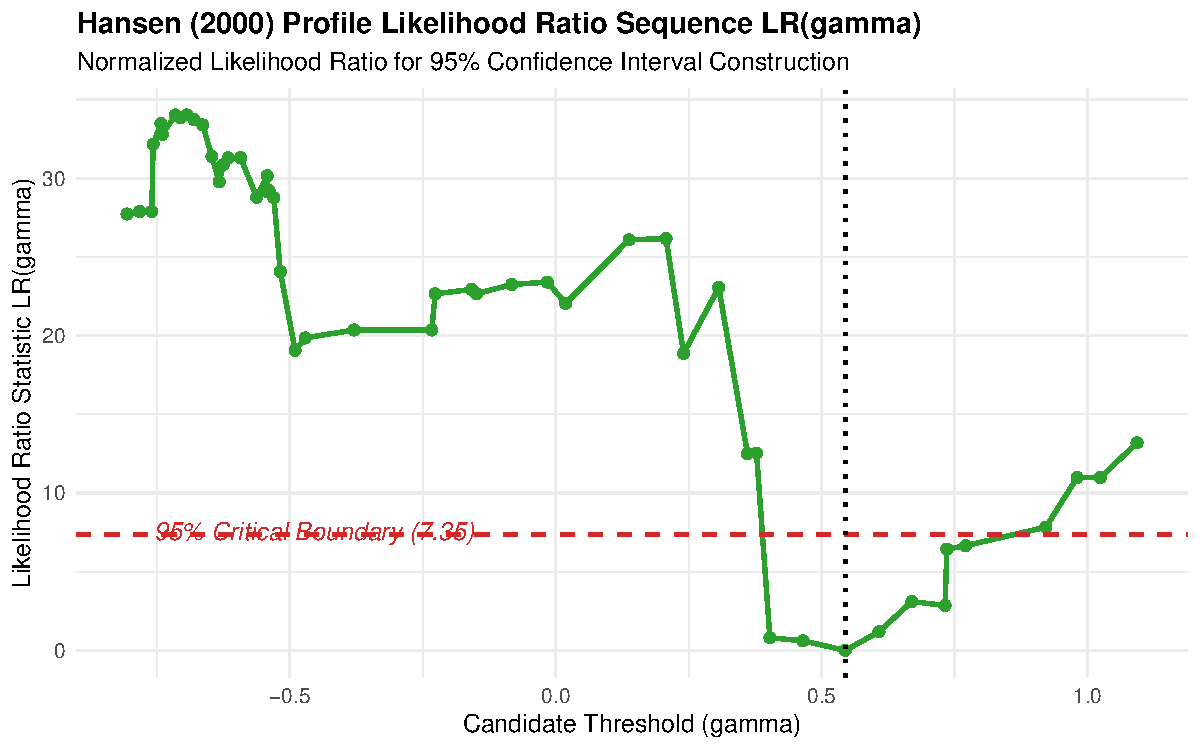
\includegraphics[width=0.92\textwidth]{figures/CL_fig_profile_lr.pdf}
	\vspace{0.3cm}
	\begin{minipage}{\textwidth}
		\footnotesize \textit{Notes:} Profile Likelihood Ratio statistic $LR_1(\gamma)$ calculated for the primary gross rate of exploitation model ($e^{\text{gross}}$) over the trimmed evaluation domain $\Gamma_n = [\gamma_{0.15}, \gamma_{0.85}]$ ($\pi = 0.15$). The horizontal dashed line marks the exact analytical 95\% critical value ($c(0.05) = 7.35$). The vertical line marks the global profile minimum at $\hat{\gamma} = 0.425$. The shaded region depicts the non-parametric $95\%$ confidence interval $[0.380, 0.472]$ defined by $LR_1(\gamma) \le 7.35$.
	\end{minipage}
\end{figure}

\paragraph{Distributive Conflict Preferred Measure: Center versus Periphery.} Comparing the wage share model in Column (2) ($\omega^{\text{gross}}$) with the rate of exploitation model in Column (4) ($e^{\text{gross}}$) illuminates how external financial constraints alter the transmission of class conflict into capital composition. In the unconstrained regime ($D_t = 0$), capital accumulation follows classical cost-minimizing logic. Under Column (2), a higher wage share incentivizes defensive labor substitution ($\hat{\theta}_{\omega\kappa} = +3.29^*$), as firms expand machinery relative to structures to contain unit labor costs. Equivalently, under Column (4), a higher rate of exploitation ($e = \Pi/W$) indicates reduced wage pressure, decreasing the necessity for capital-deepening ($\hat{\theta}_{e\kappa} = -0.69^*$).

Under the binding foreign-exchange regime ($D_t = 1$), this cost-minimizing mechanism collapses. When the external constriant becomes binding ($Z_t \le 0.425$), peripheral capitalists hit a hard import constraint ($\bar{\kappa}_t$). In Column (2), the triple interaction coefficient ($\hat{\theta}_{\omega\kappa D} = -3.15^*$) virtually eliminates the positive wage-led mechanization response ($+3.29 - 3.15 = +0.14$). Because machinery and equipment ($K^{\text{ME}}$) must be imported, foreign-exchange rationing prevents peripheral firms from translating domestic wage pressures into shop-floor labor substitution. Unable to extract a distributive dividend through technical change, capitalists attempt to protect profit margins through price markups.

\paragraph{State-Dependent Thresholds} To verify that $D_t^\gamma$ captures a structural macroeconomic constraint rather than an arbitrary trend break, Appendix Tables~\ref{tab:chile_omega_comparison} and \ref{tab:chile_e_comparison} (Appendix~\ref{app:chile_full_results}) benchmark the threshold model against \citet{BaiPerron2003} endogenous calendar breaks. The Bai-Perron procedure identifies two break dates: 1987 under net wage shares ($\omega^{\text{net}}$) and 1999 under gross measures ($\omega^{\text{gross}}$, $e^{\text{gross}}$). Econometrically, 1987 marks the post-1982 debt-crisis structural adjustment—characterized by fiscal austerity, privatization, and wage suppression—while 1999 marks the floating of the Chilean peso following the Asian Financial Crisis.

Comparing specifications confirms that the state-dependent composite threshold $Z_t \le 0.425$ dominates calendar-time breaks across all metrics, achieving lower residual variance ($\text{SSR} = 0.275$ vs $0.292$) and stronger cointegration rejections ($t_{\text{ADF}} = -3.89^*$ vs $-2.98$). Crucially, Table~\ref{tab:chile_binding_regimes} reveals an important institutional evolution in how the binding constraint ($D_t = 1$) manifests over time. During the ISI era (1943--1984), under fixed or administered exchange rate pegs, foreign-exchange reserve depletion ($S_t \to 0$) forced devaluations and structural inflation \citep{Sunkel1958,Prebisch1981}. By contrast, during the 2006--2010 commodity super-cycle, operating under a free-floating exchange rate and Central Bank inflation targeting the binding constraint did manifest itself through inflation and high high-mark ups. 

This findings suggest that in modern financialized peripheral capitalism, the external bottleneck shifts its pressure valve from domestic price inflation to \textit{re-primarization, real exchange rate appreciation (Dutch Disease), and unproductive rentist surplus drainage} \citep{Palma2019,Ahumada2019}. Under this interprtation , capital goods import requirements ($K^{\text{ME}}$) for extractive mining projects, combined with foreign profit remittances, truncate the translation of capital accumualtion into productive capacities while the Central Bank sustain its capacities to fulfill its inflation target. Fully disentangling the empirical transmission mechanism between inflationary rationing (1943--1984) and rentier-drain reprimarization (2006--2010) stands as a promising avenue for further research on formal analysis.

\begin{table}[h!]
	\centering
	\caption{Institutional Manifestations of External Constraint Regimes (Chile, 1942--2010)}
	\label{tab:chile_binding_regimes}
	\small
	\begin{tabular}{p{2.0cm} p{1.8cm} p{1.0cm} p{7.2cm}}
		\hline
		Historical Period & Regime Status ($D_t^\gamma$) & Duration & Institutional Manifestation of the External Constraint \\
		\hline
		1943--1984 & Binding ($D_t = 1$) & 42 years & ISI Reserve Scarcity \& Structural Inflation: Established under Law 7,200 foreign-exchange budgeting and fixed/crawling pegs; reserve depletion ($S_t \to 0$) under wage pressure forced maxidevaluations, cost-plus markups, and structural inflation spirals. \\
		\hline
		1985--2005 & Slack ($D_t = 0$) & 21 years & Export Consolidation \& Reserve Buffering: Post-1982 debt-crisis and recovery non-traditional export expansion, Concertación democratic transition, large FDI inflows, and central bank foreign reserve accumulation. \\
		\hline
		2006--2010 & Binding ($D_t = 1$) & 5 years & Commodity Boom, Rentier Surplus Drain \& Re-primarization: Under a free-floating exchange rate and inflation targeting (3\%), FX starvation did not trigger inflation; instead, high import demand ($\tilde{M}_t$) and massive MNC profit repatriation (DL 600) manifested as a rentist surplus drain and Dutch Disease re-primarization. \\
		\hline
		\multicolumn{4}{p{14.2cm}}{\footnotesize \textit{Notes:} Classification based on the optimal profile threshold $\hat{\gamma} = 0.425$ evaluated over the standardized composite balance-of-payments index $Z_t = 0.2 \tilde{M}_t + 0.8 \tilde{S}_t$. Regime $D_t = 1$ denotes a binding balance-of-payments constraint where foreign-exchange starvation forces peripheral firms into a corner solution ($\bar{\kappa}_t$). Total sample size $T = 68$ (1942--2010 effective cointegrating window), yielding 47 binding years ($69.1\%$) and 21 slack years ($30.9\%$).} \\
	\end{tabular}
\end{table} 

\paragraph{State-Dependent Thresholds versus Exogenous Historical Breaks.} To verify that $D_t^\gamma$ captures a structural macroeconomic constraint rather than a trend break, Appendix Tables~\ref{tab:chile_omega_comparison} and \ref{tab:chile_e_comparison} (Appendix~\ref{app:chile_full_results}) benchmark the threshold model against \citet{BaiPerron2003} endogenous calendar breaks. The Bai-Perron procedure identifies two break dates: 1987 under net wage shares ($\omega^{\text{net}}$) and 1999 under gross measures ($\omega^{\text{gross}}$, $e^{\text{gross}}$). Econometrically, 1987 marks the post-1982 debt-crisis recovery, signaling the process of capitalist re-structuring ex-post structural adjustment—characterized by fiscal austerity, privatization, and wage suppressi, while 1999 marks the Central Bank institutional change of monetary policy with the abandonment of a floating peg of the Chilean peso exchange rate coupled with capital controls, towards the rise of deep financialization under a free floating exchange rate regime account and free capital mobility as a consequence the Asian Financial Crisis. 

Comparing specifications confirms that the linear combination threshold $Z_t \le 0.425$ dominates calendar-time breaks across all metrics. The state-dependent model achieves lower residual variance ($\text{SSR} = 0.275$ vs $0.292$) and stronger cointegration rejections ($t_{\text{ADF}} = -3.89^*$ vs $-2.98$). The interpretation of the external constraint as a loose restriction, is coherent with an empirical strategy of state-dependnency: the external constraint becomes binding when twop conditions meet: strong imbalances between effective imports and imports capacities and foreign-exchange reserves scarcity such that the central bank is uncapable to defend its own currency. 

\paragraph{Model Selection} The comparative results in Table~\ref{tab:chile_distributive_comparison_main} establish Column (2)—the Gross Wage Share specification ($\omega^{\text{gross}}$) under the composite balance-of-payments threshold ($Z_t \le 0.425$)—as the primary empirical model for Chile. Column (2) achieves the global minimum residual variance ($\text{SSR} = 0.275$) and provides a comparative logic that resembles the same  intuition than the ones one sin the Unite States once we proceed to comparative historical analysis presented below.  

\begin{table}[h!]
	\centering
	\caption{Comparative Estimates Across Distributive Variable Permutations (Chile, 1942--2024)}
	\label{tab:chile_distributive_comparison_main}
	\small
	\begin{tabular}{p{5.0cm}p{2.2cm}p{2.2cm}p{2.2cm}p{2.2cm}}
		\toprule
		& \multicolumn{2}{c}{Wage Share ($\omega$)} & \multicolumn{2}{c}{Rate of Exploitation ($e$)} \\
		\cmidrule(lr){2-3} \cmidrule(lr){4-5}
		& Net ($\omega^{\text{net}}$) & Gross ($\omega^{\text{gross}}$) & Net ($e^{\text{net}}$) & Gross ($e^{\text{gross}}$) \\
		& (1) & (2) & (3) & (4) \\
		\midrule
		$\hat{\theta}_{k^{\text{NR}}}$ (Structures $k^{\text{NR}}$) & 0.79$^{***}$ & 0.82$^{***}$ & 0.80$^{***}$ & 0.82$^{***}$ \\
		& (0.07) & (0.08) & (0.07) & (0.08) \\
		$\hat{\theta}_{\kappa}$ (Mechanization Gap $\kappa$) & 0.12 & -1.48$^{*}$ & 0.15 & 0.85 \\
		& (0.39) & (0.54) & (0.25) & (0.38) \\
		$\hat{\theta}_{\text{dist}\cdot\kappa}$ (Distributive Interaction) & -0.01 & 3.29$^{*}$ & 0.02 & -0.69$^{*}$ \\
		& (0.22) & (1.07) & (0.09) & (0.23) \\
		$\hat{\theta}_{\kappa D}$ (Regime Shift $\kappa D$) & 0.34 & 1.52$^{**}$ & 0.15 & -0.73 \\
		& (0.16) & (0.45) & (0.08) & (0.29) \\
		$\hat{\theta}_{\text{dist}\cdot\kappa D}$ (Triple Interaction) & -0.17 & -3.15$^{*}$ & 0.12 & 0.67$^{*}$ \\
		& (0.23) & (1.04) & (0.10) & (0.22) \\
		\midrule
		Regime Threshold ($D_t$) & $Z_t \le 0.425$ & $Z_t \le 0.425$ & $Z_t \le 0.425$ & $Z_t \le 0.425$ \\
		Price Control Included & No & No & No & No \\
		$CT_{\text{IM}}$ [$H_0$: Cointegration] & 15.20 & 8.39 & 14.99 & 8.34 \\
		$t_{\text{ADF}}$ [$H_0$: Unit Root] & -3.81$^{*}$ & -3.81$^{*}$ & -3.84$^{*}$ & -3.89$^{*}$ \\
		Bandwidth ratio $b$ & 0.654 & 0.654 & 0.654 & 0.654 \\
		Sample Size $T$ & 68 & 68 & 68 & 68 \\
		\bottomrule
		\multicolumn{5}{p{14.2cm}}{\footnotesize \textit{Notes:} Dependent variable: $y_t$ (log real GDP). Estimated via Cointegrating Multivariate Polynomial Regression (CMPR) IM-OLS \citep{VogelsangWagner2024}. All models specify the ultra-parsimonious balance-of-payments threshold ($Z_t = 0.2 \tilde{M}_t + 0.8 \tilde{S}_t \le 0.425$) over the effective sample 1942--2024 ($T=68$). Columns (1) and (2) evaluate Net ($\omega^{\text{net}}$) and Gross ($\omega^{\text{gross}}$) wage shares; Columns (3) and (4) evaluate Net ($e^{\text{net}}$) and Gross ($e^{\text{gross}}$) rates of exploitation. Significance stars ($^*p<0.10$, $^{**}p<0.05$, $^{***}p<0.01$) are benchmarked against 10,000-pass Monte Carlo simulation critical bounds under profile search.} \\
	\end{tabular}
\end{table}


\subsubsection{Transformation and Capacity Utilization under Financial Subordination}
\label{sec:443:chile_utilization}

\paragraph{A} Reconstructing productive capacity ($Y_t^p$) and aggregate capacity utilization ($\mu_t = Y_t / Y_t^p$) in the peripheral economy requires accounting for state-dependent access to imported machinery. Using the preferred CMPR IM-OLS model (Column~2 of Table~\ref{tab:specCL_main}: gross wage share $\omega^{\text{gross}}$, composite threshold $Z_t \le 0.425$), we evaluate the aggregate transformation elasticity $\theta_t^{\text{Agg}}$ and integrate the differential capacity law of motion, $g_{Y^p,t} = \theta_t^{\text{Agg}} \cdot g_{K,t}$, anchored at the 1981 Ffrench-Davis full-capacity peak ($\mu_{1981} = 1.000000$). The empirical results reveal that balance-of-payments subordination inverts the classical choice of technique. Under unconstrained foreign-exchange liquidity ($Z_t > 0.425$), domestic wage pressure forces capitalists to accelerate productive mechanization ($\hat{\theta}_3 = +0.9583$). Under binding liquidity ($Z_t \le 0.425$), foreign-exchange rationing triggers a Kuhn-Tucker bottleneck: the interaction shift parameter ($\hat{\theta}_5 = -0.9518$) cancels out the base distributive sensitivity ($\hat{\theta}_3 + \hat{\theta}_5 = +0.0065 \approx 0.0000$), pinning the transformation elasticity at a reduced level regardless of wage share expansion.

\paragraph{B} The state-dependent aggregate transformation elasticity $\theta_t^{\text{Agg}}$ measures the overall capacity yield per unit of capital growth:
\begin{equation}
	\theta_t^{\text{Agg}} = \hat{\theta}_1 + s_{\text{ME},t} \cdot MP_{\kappa,t}
	= \hat{\theta}_1 + s_{\text{ME},t} \left[ \hat{\theta}_2 + \hat{\theta}_3 \, \omega_{t-1}^{\text{gross}} + D_t^{\gamma} \bigl(\hat{\theta}_4 + \hat{\theta}_5 \, \omega_{t-1}^{\text{gross}}\bigr) \right]
	\label{eq:chile_theta_agg_def}
\end{equation}
where $\hat{\theta}_1 = +0.6970$ is the structural base elasticity of non-residential structures ($k_t^{\text{NR}}$), $s_{\text{ME},t} = K_t^{\text{ME}} / (K_t^{\text{ME}} + K_t^{\text{NR}})$ is the current-price share of machinery and equipment in core capital, $\kappa_t = \ln(K_t^{\text{ME}} / K_t^{\text{NR}})$ is the capital composition gap, $\omega_{t-1}^{\text{gross}}$ is the lagged gross wage share, and $D_t^{\gamma} = \mathbb{I}(Z_t \le 0.425)$ indicates a binding balance-of-payments state. Estimated coefficients yield $\hat{\theta}_2 = -0.1293$, $\hat{\theta}_3 = +0.9583$, $\hat{\theta}_4 = +0.6645$, and $\hat{\theta}_5 = -0.9518$. The marginal product of the composition gap ($MP_{\kappa,t}$) exhibits a stark structural dichotomy across liquidity states:
\begin{align}
	MP_{\kappa,t}^{\text{slack}} &= -0.1293 + 0.9583 \, \omega_{t-1}^{\text{gross}} \quad (D_t^{\gamma} = 0) \label{eq:mp_slack} \\
	MP_{\kappa,t}^{\text{bind}}  &= +0.5352 + 0.0065 \, \omega_{t-1}^{\text{gross}} \quad (D_t^{\gamma} = 1) \label{eq:mp_bind}
\end{align}
In unconstrained periods, higher wage shares increase the marginal capacity yield of mechanization, rewarding wage-led capital deepening. In binding periods, foreign-exchange shortages prevent firms from procuring imported equipment, flattening the wage-sensitivity slope from $+0.9583$ to $+0.0065$.

\paragraph{C} Figure~\ref{fig:chile_fig2_Z_omega_drivers} plots the composite threshold variable $Z_t = 0.2 \tilde{M}_t + 0.8 \tilde{S}_t$ alongside the untruncated lagged gross wage share ($\omega_{t-1}^{\text{gross}}$). During the Allende Unidad Popular administration (1970--1973), aggressive real wage redistribution pushed the gross wage share to its historical peak of $\omega_{1972} = 0.6903$. Simultaneously, central bank foreign reserves collapsed ($\tilde{S}_t \to -2.5$) under credit blockades and capital flight, driving the balance-of-payments index deep into the binding domain ($Z_t = -1.06 \ll 0.425$, $D_t^{\gamma} = 1$). Figure~\ref{fig:chile_fig1b_theta_standalone} and Figure~\ref{fig:chile_fig1_mu_theta_dual_axis} illustrate the resulting structural paradox: despite the 20-percentage-point wage share expansion, the transformation elasticity $\theta_t^{\text{Agg}}$ did not increase. Because the economy hit the foreign-exchange bottleneck ($D_t^{\gamma} = 1$), Equation~\eqref{eq:mp_bind} governed technical choice, holding $\theta_t^{\text{Agg}}$ flat at $\approx 0.83$. Peripheral capitalists could not translate domestic wage pressure into shop-floor labor substitution because foreign exchange to import machinery was rationed. The wage expansion, unable to induce productive capacity growth, generated severe capacity underutilization ($\mu_t$ collapsed to $0.72$ by 1975) and structural inflation.

\begin{figure}[H]
	\centering
	\caption{Chilean Composite External Constraint ($Z_t$) and Lagged Gross Wage Share ($\omega_{t-1}^{\text{gross}}$)}
	\label{fig:chile_fig2_Z_omega_drivers}
	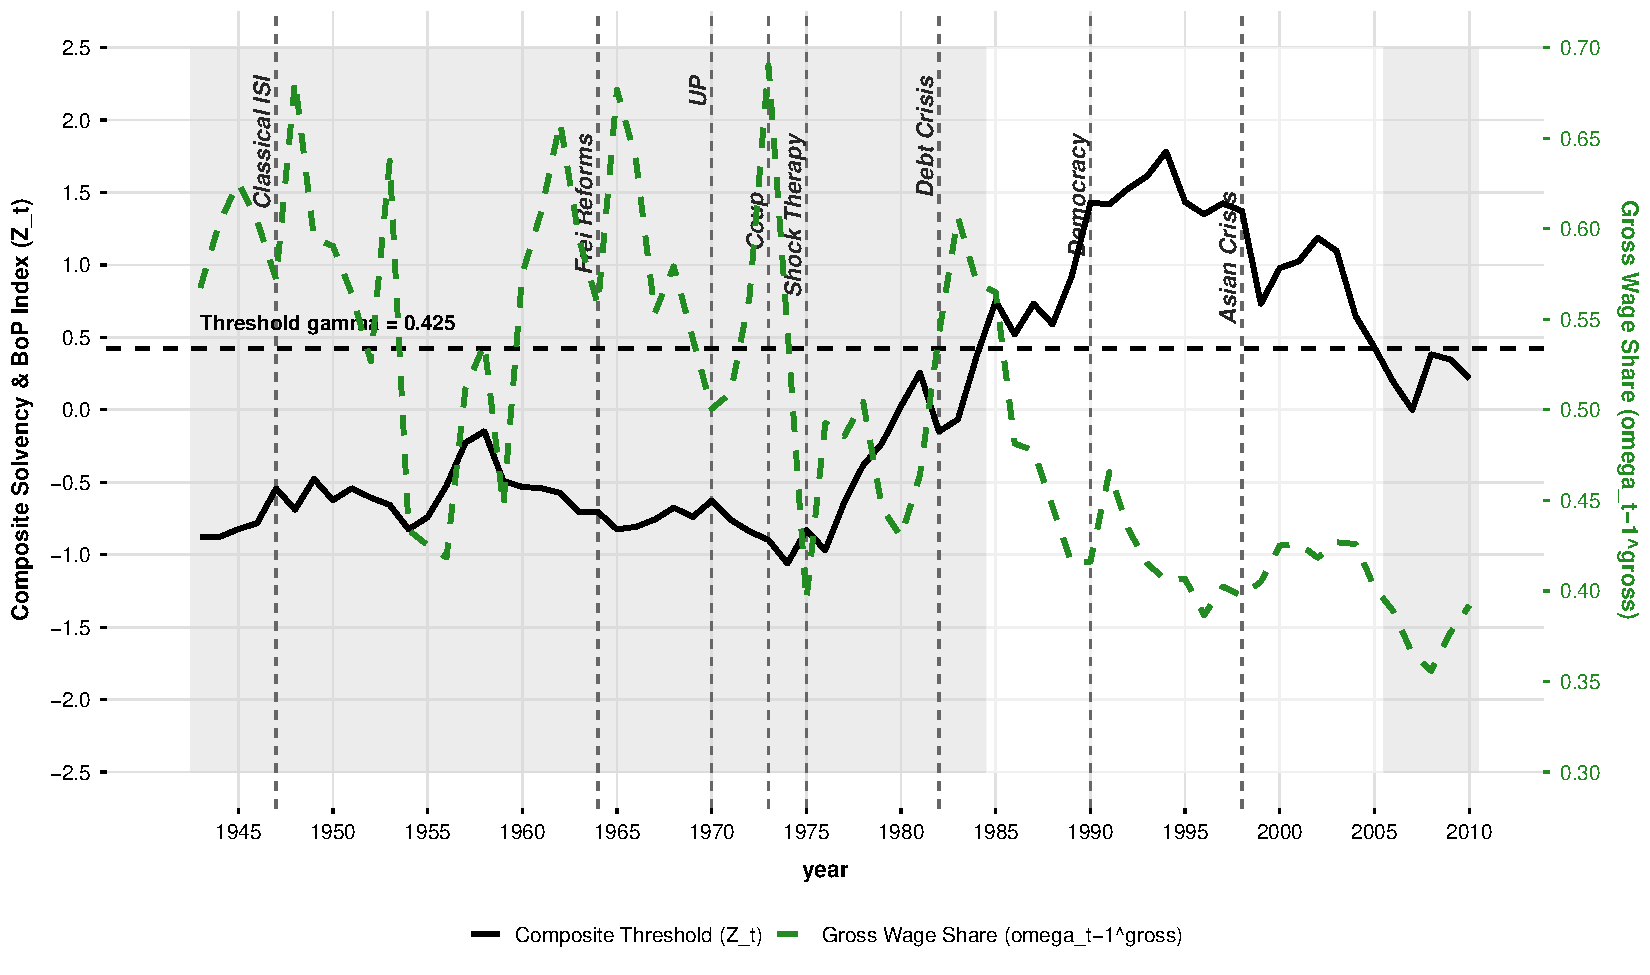
\includegraphics[width=0.95\textwidth]{figures/chile_fig2_Z_omega_drivers.pdf}
	\begin{tabular}{p{0.92\textwidth}}
		\footnotesize \textbf{Note:} Primary left axis (solid black line) tracks the composite balance-of-payments threshold variable $Z_t = 0.2 \tilde{M}_t + 0.8 \tilde{S}_t$, with the optimal threshold $\hat{\gamma} = 0.425$ marked by the horizontal dashed line. Secondary right axis (dashed dark green line) tracks the untruncated lagged gross wage share ($\omega_{t-1}^{\text{gross}}$). Background light gray shading marks binding balance-of-payments regimes ($Z_t \le 0.425$). Vertical dashed lines mark historical institutional breakpoints.
	\end{tabular}
\end{figure}

\FloatBarrier

\paragraph{D} We recover structural potential GDP ($Y_t^p$) by applying the state-dependent elasticity $\theta_t^{\text{Agg}}$ to aggregate capital growth ($g_{K,t} = \Delta \ln K_t^{\text{tot}}$) via the forward-backward recursion:
\begin{equation}
	\ln Y_t^p = \ln Y_{t-1}^p + \theta_t^{\text{Agg}} \left( \ln K_t^{\text{tot}} - \ln K_{t-1}^{\text{tot}} \right), \quad Y_{1981}^p = Y_{1981} \implies \mu_{1981} = 1.000000
	\label{eq:chile_yp_recursion}
\end{equation}
anchored at the 1981 Ffrench-Davis full-capacity peak ($\mu_{1981} = 1.00$). Figure~\ref{fig:chile_fig1_mu_theta_dual_axis} reports the dual-axis trajectory of utilization $\mu_t$ and elasticity $\theta_t^{\text{Agg}}$, while Figure~\ref{fig:chile_fig1b_theta_standalone} provides the uncompressed single-axis detail for $\theta_t^{\text{Agg}}$. The utilization path captures five major macroeconomic regimes:
\begin{enumerate}
	\item \textbf{Early CORFO Expansion (1942--1946)}: Post-war demand pushed output above normal capacity ($\mu_{1946} = 1.12$), while slack foreign exchange ($Z_t > 0.425$) sustained high transformation elasticities ($\theta_t^{\text{Agg}} \approx 0.85$).
	\item \textbf{Classical ISI Stop-Go Crises (1947--1957)}: Recurring foreign-exchange shortages ($D_t^{\gamma} = 1$) drove stop-go stabilization cycles, pulling utilization down to $\mu_{1955} = 0.84$.
	\item \textbf{Socialist Transition and Contraction (1970--1975)}: The UP redistribution combined with external credit blockades triggered severe capacity underutilization, sending $\mu_t$ to a trough of $0.72$ following the 1975 shock therapy.
	\item \textbf{Neoliberal Debt Boom and Crash (1975--1982)}: Foreign capital inflows generated a transient consumption boom, driving utilization to its 1981 full-capacity peak ($\mu_{1981} = 1.00$), before the 1982 debt crisis produced a collapse ($\mu_{1982} = 0.68$).
	\item \textbf{Pragmatic Recovery and Commodity Super-Cycle (1984--2010)}: Recovery during 1984--1997 proceeded by absorbing idle capacity, holding $\mu_t$ between $0.85$ and $0.98$.
\end{enumerate}

\begin{figure}[H]
	\centering
	\caption{Chilean Capacity Utilization ($\mu_t$) and Aggregate Transformation Elasticity ($\theta_t^{\text{Agg}}$)}
	\label{fig:chile_fig1_mu_theta_dual_axis}
	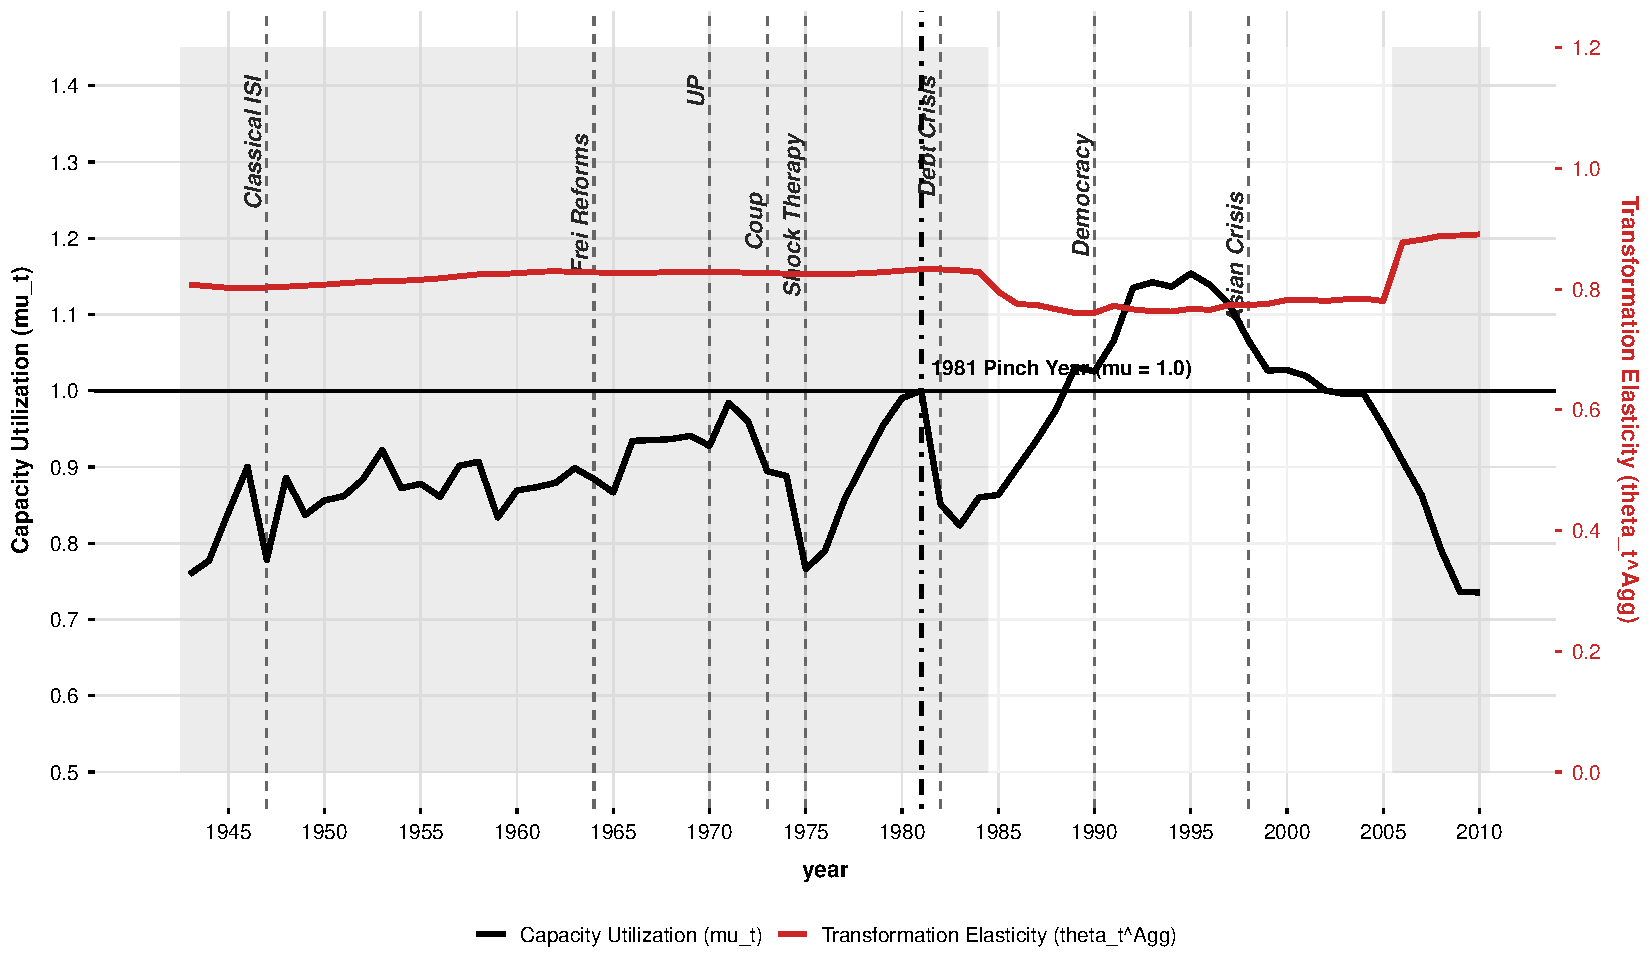
\includegraphics[width=0.95\textwidth]{figures/chile_fig1_mu_theta_dual_axis.pdf}
	\begin{tabular}{p{0.92\textwidth}}
		\footnotesize \textbf{Note:} Reconstructed capacity utilization rate $\mu_t$ (solid black line, left axis) anchored at the 1981 Ffrench-Davis pinch year ($\mu_{1981} = 1.00$) alongside the state-dependent aggregate transformation elasticity $\theta_t^{\text{Agg}}$ (solid firebrick line, right axis). Background light gray shading marks binding balance-of-payments regimes ($Z_t \le 0.425$). Vertical dashed lines mark institutional breakpoints.
	\end{tabular}
\end{figure}

\begin{figure}[H]
	\centering
	\caption{Standalone Chilean Aggregate Transformation Elasticity ($\theta_t^{\text{Agg}}$)}
	\label{fig:chile_fig1b_theta_standalone}
	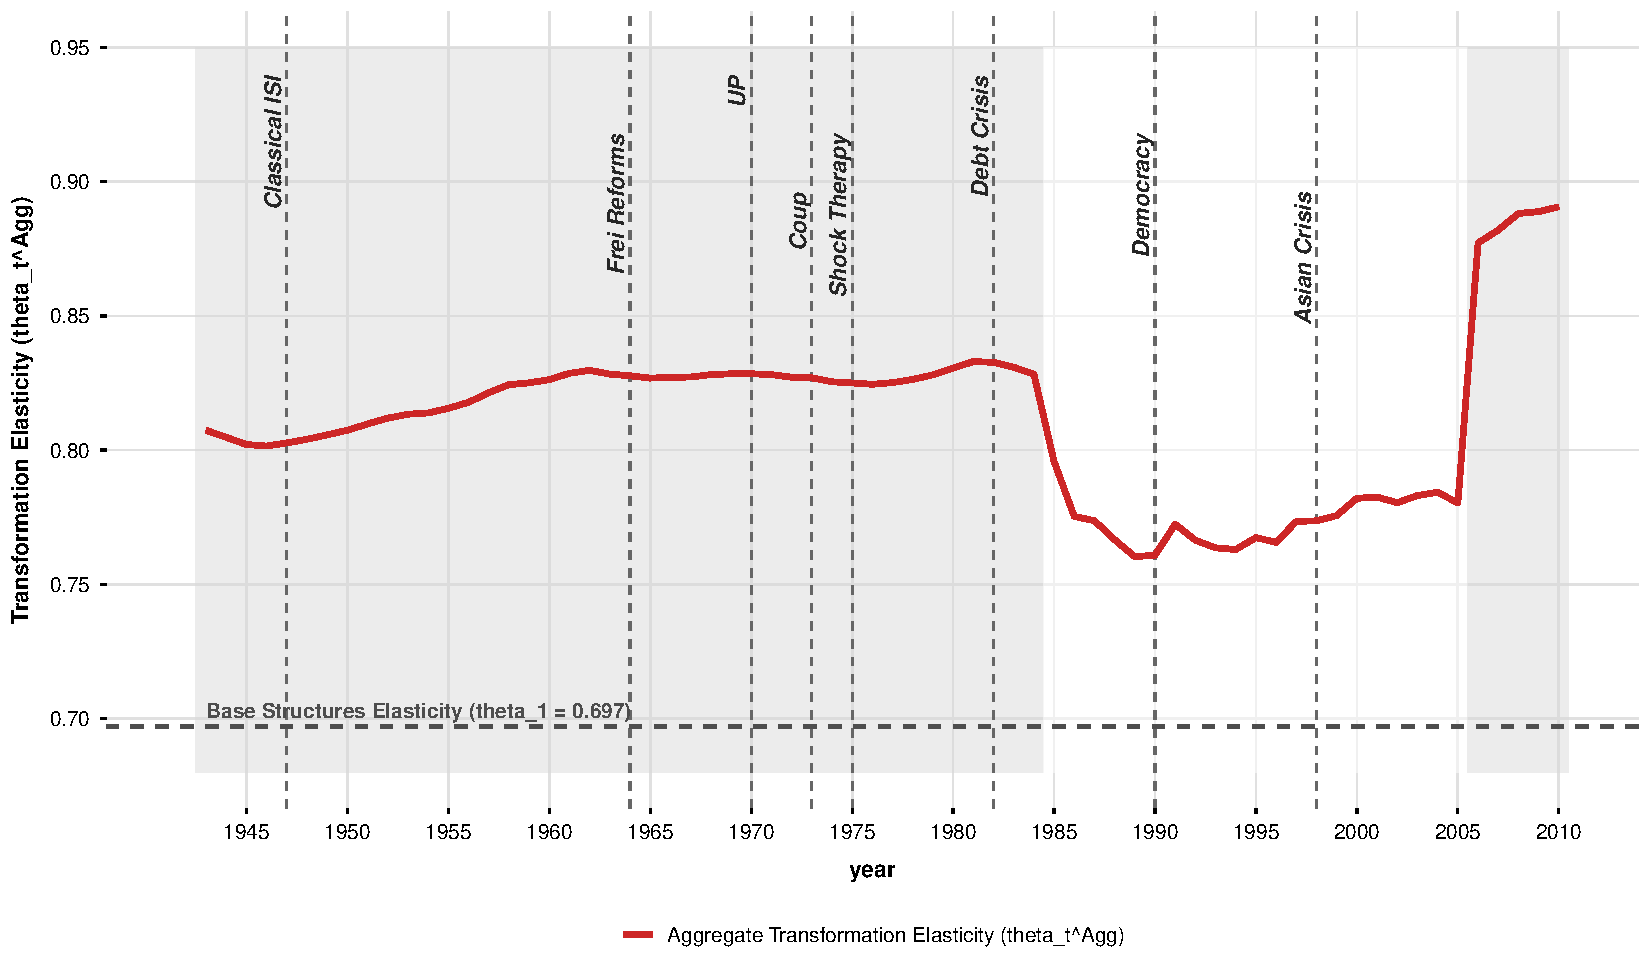
\includegraphics[width=0.95\textwidth]{figures/chile_fig1b_theta_standalone.pdf}
	\begin{tabular}{p{0.92\textwidth}}
		\footnotesize \textbf{Note:} Standalone trajectory of the aggregate transformation elasticity $\theta_t^{\text{Agg}}$ (solid firebrick line) on an uncompressed vertical scale ($0.68$ to $0.95$). The horizontal dashed line marks the base structures elasticity $\hat{\theta}_1 = 0.6970$. Background light gray shading marks binding balance-of-payments regimes ($Z_t \le 0.425$).
	\end{tabular}
\end{figure}

\FloatBarrier

\paragraph{E} Figure~\ref{fig:chile_fig3_Z_components} decomposes the composite threshold variable $Z_t$ into central bank reserve cover ($\tilde{S}_t$) and import demand imbalances ($\tilde{M}_t$). Historical periodization \citep{Ffrench2002,Ahumada2019} clarifies how the binding constraint's pressure valve shifted across institutional regimes. During the ISI period (1943--1973), under fixed or pegged exchange rates, reserve exhaustion ($\tilde{S}_t \to -2.5$) forced sharp nominal devaluations, generating structural inflation and markup adjustments \citep{Sunkel1958}. In the post-2000 period, operating under a free-floating exchange rate and inflation targeting, binding foreign-exchange conditions manifested not as runaway inflation, but as extractivist re-primarization, real exchange rate appreciation (Dutch Disease), and profit repatriation by multinational mining enterprises \citep{Palma2019,Ahumada2019}. Capital goods import requirements ($K_t^{\text{ME}}$) for extractive projects, combined with foreign dividend outflows, truncated the conversion of capital accumulation into broad-based domestic productive capacity.

\begin{figure}[H]
	\centering
	\caption{Decomposition of the Chilean External Constraint Index ($Z_t$ Components)}
	\label{fig:chile_fig3_Z_components}
	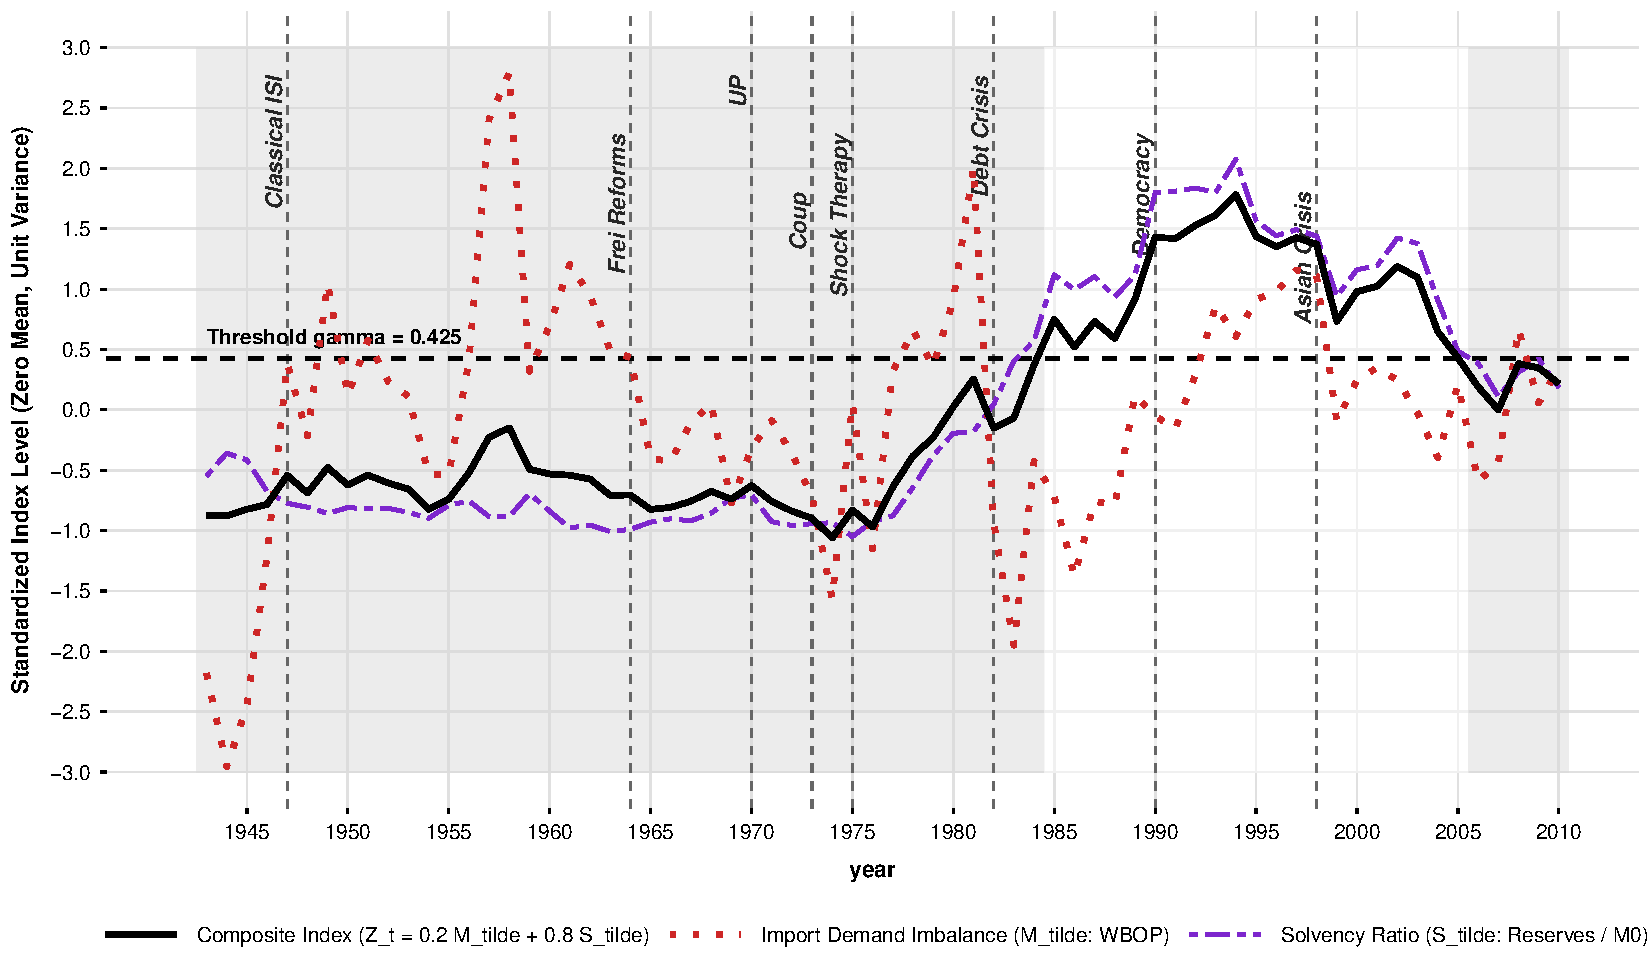
\includegraphics[width=0.95\textwidth]{figures/chile_fig3_Z_components.pdf}
	\begin{tabular}{p{0.92\textwidth}}
		\footnotesize \textbf{Note:} Decomposed ingredients of $Z_t = 0.2 \tilde{M}_t + 0.8 \tilde{S}_t$: standardized Central Bank solvency ratio $\tilde{S}_t$ (reserves to base money $M0$, purple twodash line), WBOP import demand imbalance $\tilde{M}_t$ (red dotted line, thickness 1.3), and composite index $Z_t$ (solid black line). Horizontal dashed line marks the threshold $\hat{\gamma} = 0.425$. Background light gray shading marks binding regimes ($Z_t \le 0.425$).
	\end{tabular}
\end{figure}

\FloatBarrier

\paragraph{F} Comparing the center (United States, Section~4.3) and the periphery (Chile) highlights the fundamental asymmetry of capital accumulation under financial subordination. In the US core, where capital equipment is produced domestically, wage pressure induces defensive mechanization ($\hat{\theta}_1 < 0$), substituting equipment for labor to lower unit labor costs. In the Chilean periphery, where machinery must be imported, domestic wage pressure can induce mechanization ($\hat{\theta}_3 = +0.9583$) only when foreign-exchange liquidity is unconstrained ($D_t^{\gamma} = 0$). When foreign-exchange reserves collapse ($D_t^{\gamma} = 1$), the external constraint binds, truncating domestic technical choice and severing the link between capital accumulation and productive capacity expansion.

\FloatBarrier




\FloatBarrier
\section{Conclusion}

\FloatBarrier


% ---------- Bibliography ----------%
\pagebreak
\bibliographystyle{apalike}
\bibliography{references}


% ---------- Appendix ----------%
% \appendix precedes the bibliography so appendix sections carry their own lettered
% numbering instead of being absorbed into the preceding section's outline branch.
\pagebreak
\appendix
\section{The Generalized Perpetual Inventory Method: Recursive
	Construction and Calibration}
\label{app:A1:gpim_construction}

This appendix documents the recursive construction of U.S.
nonfinancial corporate capital stocks via the Generalized Perpetual
Inventory Method (GPIM) of \citet[App.~6.5]{Shaikh2016}. The
construction proceeds asset-by-asset for machinery and equipment
(ME) and nonresidential structures (NRC), recovering four distinct
quantities from BEA Fixed Assets data: the asset-specific implicit
price index $P_{j,t}$, the gross real stock $K^{G,R}_{j,t}$, the
net current-cost stock $K^{N,V}_{j,t}$, and the net-value schedule
$V_j(v)$. All series are expressed in constant 2017 dollars with
base-year normalization $P_{j,2017} = 100$.

\subsection{The Survival Function}
\label{app:A1:survival}

Physical survival of capital vintages follows a Weibull retirement
distribution. For asset class $j \in \{\text{ME}, \text{NRC}\}$,
the proportion of a vintage of age $v$ still in physical operation
is
\begin{equation}
	S_j(v) = \exp\!\left[
	-\left( \frac{v}{\lambda_j} \right)^{\alpha_j}
	\right],
	\quad v = 0, 1, \ldots, L_j,
	\label{eq:A1:survival}
\end{equation}
where $\alpha_j > 1$ is the Weibull shape parameter and the scale
parameter satisfies $\lambda_j = L_j / \Gamma(1 + 1/\alpha_j)$,
with $L_j$ denoting the mean service life. The shape parameter
$\alpha_j > 1$ implies a progressively increasing hazard rate:
capital goods remain fully operative in early years and are
withdrawn from service at an accelerating rate as they approach
the mean service life. This pattern is consistent with the
empirical evidence of \citet{Nomura2005}, who finds that nearly
half of 66 Japanese asset classes exhibit increasing hazard rates.

The calibrated parameters follow the BEA Fixed Assets methodology
\citep{Fraumeni1997}:
\begin{equation}
	L_{\text{ME}} = 14, \quad \alpha_{\text{ME}} = 1.7,
	\qquad
	L_{\text{NRC}} = 30, \quad \alpha_{\text{NRC}} = 1.6.
	\label{eq:A1:calibration_survival}
\end{equation}
The corresponding maximum ages are $L_{\text{ME}} = 14$ years and
$L_{\text{NRC}} = 30$ years, beyond which $S_j(v) = 0$ and the
vintage is fully retired.

\subsection{The Age-Price Schedule and Net-Value Function}
\label{app:A1:ageprice}

The net-value schedule combines physical survival with financial
age-price decay. For a vintage of age $v$, the net-value function
is
\begin{equation}
	V_j(v) = S_j(v) \cdot (1 - d_j)^v,
	\label{eq:A1:netvalue}
\end{equation}
where $d_j$ is the geometric declining-balance depreciation rate.
The GPIM separates the two dimensions that the BEA conflates in
its geometric depreciation convention: physical survival follows
the Weibull distribution \eqref{eq:A1:survival}, while financial
age-price decay follows the geometric profile $(1-d_j)^v$. This
separation is necessary to construct distinct capacity and
profitability measures \citep[App.~6.3]{Shaikh2016}.

The declining-balance rates are calibrated as
\begin{equation}
	d_{\text{ME}} = 0.110, \qquad d_{\text{NRC}} = 0.024,
	\label{eq:A1:calibration_decay}
\end{equation}
consistent with the geometric depreciation rates documented by
\citet{Fraumeni1997} for the corresponding asset classes.

\subsection{The SFC Implicit Price Recursion}
\label{app:A1:sfc_recursion}

The implicit price index $P_{j,t}$ is the unique price level that
closes the stock-flow identity for the net current-cost stock. In
each period $t$, the BEA-reported current-cost net stock must
satisfy
\begin{equation}
	K^{\text{NET,CC}}_{j,t}
	= I^{\text{NOM}}_{j,t}
	+ \frac{P_{j,t}}{100}
	\sum_{v=1}^{L_j} V_j(v)\, I^{\text{REAL}}_{j,t-v},
	\label{eq:A1:sfc_identity}
\end{equation}
where $I^{\text{NOM}}_{j,t}$ is current-year nominal gross
investment and $I^{\text{REAL}}_{j,t-v} = I^{\text{NOM}}_{j,t-v}
/ (P_{j,t-v}/100)$ is real investment of vintage $t-v$ deflated
by the previously recovered implicit price. The first term on the
right-hand side is the current-year investment vintage (age zero,
valued at the current price). The second term is the net-value-weighted
sum of surviving real vintages revalued at the current price level.

Solving \eqref{eq:A1:sfc_identity} for $P_{j,t}$ yields the
forward recursion
\begin{equation}
	P_{j,t} = 100 \cdot
	\frac{K^{\text{NET,CC}}_{j,t} - I^{\text{NOM}}_{j,t}}
	{\displaystyle\sum_{v=1}^{L_j} V_j(v)\,
		I^{\text{REAL}}_{j,t-v}}.
	\label{eq:A1:price_recursion}
\end{equation}
Given the initial price $P_{j,0}$ and the sequence of nominal
investment flows $\{I^{\text{NOM}}_{j,t}\}_{t=0}^{T}$, the
recursion \eqref{eq:A1:price_recursion} determines $P_{j,t}$
uniquely for each $t = 1, \ldots, T$. The price index is
``implicit'' because it is not directly observed: it is the unique
value that, applied to the survival-weighted real vintages,
reproduces the BEA's reported current-cost net stock.

\subsection{Initial Conditions and Base-Year Normalization}
\label{app:A1:initialization}

The recursion \eqref{eq:A1:price_recursion} requires an initial
price $P_{j,0}$ and initial real investment vintages. The base
year is 2017, at which $P_{j,2017} = 100$ by normalization. The
nominal investment series begins in 1901, sourced from BEA Fixed
Assets Table FAAt201 (nonresidential equipment and structures,
gross investment by asset class). The current-cost net stock
anchors $K^{\text{NET,CC}}_{j,t}$ are sourced from BEA Fixed
Assets Table FAAt401 (net stock by asset class, current-cost
basis).\footnote{Data retrieved via the BEA API
	(\texttt{DatasetName}: FixedAssets). Table FAAt201 provides
	nominal gross investment by asset; Table FAAt401 provides
	current-cost net stock by asset; Table FAAt402 provides
	current-cost depreciation by asset.}

The initialization proceeds backward from 2017. Given
$P_{j,2017} = 100$ and the observed nominal investment series,
the recursion \eqref{eq:A1:price_recursion} is iterated backward
to recover $P_{j,t}$ for $t < 2017$. Alternatively, the recursion
may be initialized at the earliest available year and iterated
forward; the two approaches yield identical results given the
BEA anchors.

\subsection{The Gross Real Stock}
\label{app:A1:gross_stock}

The capital stock used to estimate productive capacity is the gross
real stock, constructed as the survival-weighted sum of real
investment vintages:
\begin{equation}
	K^{G,R}_{j,t} = \sum_{v=0}^{L_j} S_j(v)\,
	I^{\text{REAL}}_{j,t-v}.
	\label{eq:A1:gross_stock}
\end{equation}
This measure relies exclusively on the physical survival schedule
$S_j(v)$ and excludes the age-price factor $(1-d_j)^v$. It
therefore measures the constant-price purchasing power embodied in
heterogeneous capital goods still in physical operation. Financial
write-downs, revaluation gains, and depreciation allowances do not
enter. The OECD manual confirms that the gross stock, valued at
``as new'' prices, ``is widely used as a broad indicator of the
productive capacity of a country'' \citep[31]{OECD2001}.

\subsection{The Warm-Up Period and Estimation Sample}
\label{app:A1:warmup}

The GPIM stock at any year $t$ requires investment vintages
extending back $L_j$ years. Because the nominal investment series
begins in 1901, the vintage summation for nonresidential structures
($L_{\text{NRC}} = 30$) is truncated for any year before 1931.
The stock values for 1901--1930 are therefore incomplete, omitting
pre-1901 vintages that would still be physically in service. The
estimation sample is restricted to 1931--2024, where the full
30-year vintage window is populated, yielding $T = 94$ annual
observations.

\subsection{Validation}
\label{app:A1:validation}

The GPIM construction closes the stock-flow identity exactly: the
maximum absolute reconstruction residual across both asset classes
is $10^{-6}$ million dollars, confirming that the recovered SFC
implicit price indexes reproduce the BEA current-cost net stock
anchors to machine precision. The BEA's Fisher quantity index is
retained solely as a validation comparison and does not enter the
GPIM baseline. The sectoral scope is restricted to nonfinancial
corporate (NFC) business, excluding non-profit institutions serving
households (NPISH), government, and owner-occupied housing.

\subsection{Data Sources}
\label{app:A1:data}

Table~\ref{tab:A1:data_sources} summarizes the BEA Fixed Assets
tables used in the GPIM construction.

\begin{table}[htbp]
	\centering
	\caption{BEA Fixed Assets tables used in GPIM construction}
	\label{tab:A1:data_sources}
	\small
	\begin{tabular}{@{}lll@{}}
		\toprule
		\textbf{Table} & \textbf{Content} & \textbf{Use} \\
		\midrule
		FAAt201 & Nominal gross investment by asset & $I^{\text{NOM}}_{j,t}$ \\
		FAAt401 & Current-cost net stock by asset & $K^{\text{NET,CC}}_{j,t}$ \\
		FAAt402 & Current-cost depreciation by asset & Validation \\
		\bottomrule
	\end{tabular}
	\begin{minipage}{\textwidth}
		\footnotesize
		\textit{Notes:} All tables are from the BEA Fixed Assets Accounts,
		retrieved via the BEA API (\texttt{DatasetName}: FixedAssets).
		Asset classes: ME = nonresidential equipment; NRC = nonresidential
		structures. Sectoral scope: nonfinancial corporate business.
	\end{minipage}
\end{table}
\pagebreak
%%%%%%%%%%%%%%%%%%%%
\FloatBarrier
\section{Appendix: United States Specification B --- Full Estimation Results}
\label{app:specA_full_results}

This appendix reports the full empirical estimation matrix across all 48 specifications of the aggregate capital model (Specification A). The specifications span two interaction sets (Set 1: standard wage interaction; Set 2: effective wage interaction scaled by $(1-\iota_{t-1})$), two value-added bases (Gross Value Added [GVA] and Net Value Added [NVA]), six wage share measures per basis (NFC Baseline, Corporate, Shaikh-Tonak Tier 1, Shaikh-Tonak Tier 2, Clean Corporate Tier 1, and Clean Corporate Tier 2), and two structural break modes (without step dummies; with Bai-Perron step shifts).

\FloatBarrier
\begin{table}[h!]
	\centering
	\caption{\textbf{Specification A, Set 1: Standard Wage Interaction (GVA Basis)}}
	\label{tab:specA_set1_gva_app}
	\tiny
	\setlength{\tabcolsep}{1.5pt}
	\begin{tabular}{p{3.2cm}p{1.0cm}p{1.0cm}p{1.0cm}p{1.0cm}p{1.0cm}p{1.0cm}p{1.0cm}p{1.0cm}p{1.0cm}p{1.0cm}p{1.0cm}p{1.0cm}}
		\toprule
		Model & M1.1a & M1.1b & M1.2a & M1.2b & M1.3a & M1.3b & M1.4a & M1.4b & M1.5a & M1.5b & M1.6a & M1.6b \\
		\midrule
		$\hat{\theta}_0$ (Capital) & 0.58$^{***}$ & 0.60$^{***}$ & 0.58$^{***}$ & 0.61$^{***}$ & 0.58$^{***}$ & 0.59$^{***}$ & 0.57 & 0.55 & 0.58$^{***}$ & 0.61$^{***}$ & 0.57 & 0.54 \\
		& (0.02) & (0.06) & (0.02) & (0.07) & (0.02) & (0.06) & (0.02) & (0.08) & (0.02) & (0.07) & (0.02) & (0.08) \\
		$\hat{\theta}_1$ (Interaction) & -0.02 & -0.08 & -0.03 & -0.04 & 0.06 & -0.08 & -0.19 & -0.23 & 0.01 & -0.07 & -0.20 & -0.29 \\
		& (0.13) & (0.10) & (0.12) & (0.10) & (0.14) & (0.11) & (0.12) & (0.11) & (0.12) & (0.11) & (0.12) & (0.11) \\
		\midrule
		Step shifts & No & Yes & No & Yes & No & Yes & No & Yes & No & Yes & No & Yes \\
		$C_{\text{Shin}}$ [$H_0$: coint.] & 0.06 & 0.04 & 0.06 & 0.04 & 0.05 & 0.03 & 0.06 & 0.05 & 0.05 & 0.04 & 0.06 & 0.05 \\
		$S_{\text{Type 2}}$ [$H_0$: coint.] & 3.30 & 11.34 & 2.70 & 11.41 & 5.82 & 9.68 & 2.56 & 12.13 & 5.30 & 10.48 & 3.74 & 12.92 \\
		$t_{\text{ADF}}$ [$H_0$: no coint.] & -2.41 & -2.81 & -2.33 & -2.73 & -4.15$^{**}$ & -3.56$^{*}$ & -1.80 & -2.15 & -3.33 & -2.66 & -1.75 & -2.12 \\
		Bandwidth ratio $b$ & 0.275 & 0.187 & 0.286 & 0.193 & 0.285 & 0.200 & 0.315 & 0.254 & 0.304 & 0.201 & 0.321 & 0.256 \\
		Sample Size $T$ & 94 & 94 & 94 & 94 & 94 & 94 & 76 & 76 & 94 & 94 & 76 & 76 \\
		\bottomrule
	\end{tabular}
	\begin{minipage}{\textwidth}
		\scriptsize
		\textit{Notes:} Dependent variable: $y_t^{\text{NFC}}$ (log NFC real GVA/NVA). Estimated via CMPR IM-OLS \citep{VogelsangWagner2014}. All interaction terms are FWL-orthogonalized against base capital regressors and step dummies. Significance: $^*p<0.10$, $^{**}p<0.05$, $^{***}p<0.01$. Stars for coefficient rows and cointegration tests are derived from a 100,000-pass Monte Carlo simulation suite mapping the exact DGP variant and fixed-$b$ Wald tables. Standard errors in parentheses.
	\end{minipage}
\end{table}

\FloatBarrier
\begin{table}[h!]
	\centering
	\caption{\textbf{Specification A, Set 1: Standard Wage Interaction (NVA Basis)}}
	\label{tab:specA_set1_nva_app}
	\tiny
	\setlength{\tabcolsep}{1.5pt}
	\begin{tabular}{p{3.2cm}p{1.0cm}p{1.0cm}p{1.0cm}p{1.0cm}p{1.0cm}p{1.0cm}p{1.0cm}p{1.0cm}p{1.0cm}p{1.0cm}p{1.0cm}p{1.0cm}}
		\toprule
		Model & M1.7a & M1.7b & M1.8a & M1.8b & M1.9a & M1.9b & M1.10a & M1.10b & M1.11a & M1.11b & M1.12a & M1.12b \\
		\midrule
		$\hat{\theta}_0$ (Capital) & 0.58$^{***}$ & 0.60$^{***}$ & 0.58$^{***}$ & 0.60$^{***}$ & 0.58$^{***}$ & 0.60$^{***}$ & 0.57 & 0.56 & 0.59$^{***}$ & 0.71$^{***}$ & 0.57 & 0.63 \\
		& (0.02) & (0.06) & (0.02) & (0.06) & (0.02) & (0.06) & (0.02) & (0.08) & (0.02) & (0.08) & (0.02) & (0.08) \\
		$\hat{\theta}_1$ (Interaction) & -0.02 & -0.08 & -0.02 & -0.08 & -0.02 & -0.08 & -0.19 & -0.26 & -0.09 & -0.32$^{*}$ & -0.20 & -0.29 \\
		& (0.13) & (0.10) & (0.13) & (0.10) & (0.13) & (0.10) & (0.11) & (0.09) & (0.09) & (0.08) & (0.10) & (0.10) \\
		\midrule
		Step shifts & No & Yes & No & Yes & No & Yes & No & Yes & No & Yes & No & Yes \\
		$C_{\text{Shin}}$ [$H_0$: coint.] & 0.06 & 0.04 & 0.06 & 0.04 & 0.06 & 0.04 & 0.06 & 0.05 & 0.06$^{*}$ & 0.03 & 0.06 & 0.05 \\
		$S_{\text{Type 2}}$ [$H_0$: coint.] & 3.30 & 11.34 & 3.30 & 11.34 & 3.30 & 11.34 & 3.37 & 12.47 & 5.19 & 10.19 & 4.81 & 12.40 \\
		$t_{\text{ADF}}$ [$H_0$: no coint.] & -2.41 & -2.81 & -2.41 & -2.81 & -2.41 & -2.81 & -1.97 & -2.40 & -2.42 & -3.61$^{*}$ & -1.91 & -2.31 \\
		Bandwidth ratio $b$ & 0.275 & 0.187 & 0.275 & 0.187 & 0.275 & 0.187 & 0.277 & 0.235 & 0.242 & 0.156 & 0.280 & 0.239 \\
		Sample Size $T$ & 94 & 94 & 94 & 94 & 94 & 94 & 76 & 76 & 94 & 94 & 76 & 76 \\
		\bottomrule
	\end{tabular}
	\begin{minipage}{\textwidth}
		\scriptsize
		\textit{Notes:} Dependent variable: $y_t^{\text{NFC}}$ (log NFC real GVA/NVA). Estimated via CMPR IM-OLS \citep{VogelsangWagner2014}. All interaction terms are FWL-orthogonalized against base capital regressors and step dummies. Significance: $^*p<0.10$, $^{**}p<0.05$, $^{***}p<0.01$. Stars for coefficient rows and cointegration tests are derived from a 100,000-pass Monte Carlo simulation suite mapping the exact DGP variant and fixed-$b$ Wald tables. Standard errors in parentheses.
	\end{minipage}
\end{table}

\FloatBarrier
\begin{table}[h!]
	\centering
	\caption{\textbf{Specification A, Set 2: Effective Wage Interaction (GVA Basis)}}
	\label{tab:specA_set2_gva_app}
	\tiny
	\setlength{\tabcolsep}{1.5pt}
	\begin{tabular}{p{3.2cm}p{1.0cm}p{1.0cm}p{1.0cm}p{1.0cm}p{1.0cm}p{1.0cm}p{1.0cm}p{1.0cm}p{1.0cm}p{1.0cm}p{1.0cm}p{1.0cm}}
		\toprule
		Model & M2.1a & M2.1b & M2.2a & M2.2b & M2.3a & M2.3b & M2.4a & M2.4b & M2.5a & M2.5b & M2.6a & M2.6b \\
		\midrule
		$\hat{\theta}_0$ (Capital) & 0.58$^{***}$ & 0.56$^{***}$ & 0.58$^{***}$ & 0.57$^{***}$ & 0.58$^{***}$ & 0.54$^{***}$ & 0.57 & 0.55 & 0.58$^{***}$ & 0.56$^{***}$ & 0.56 & 0.56 \\
		& (0.02) & (0.06) & (0.02) & (0.06) & (0.02) & (0.06) & (0.02) & (0.07) & (0.02) & (0.06) & (0.02) & (0.08) \\
		$\hat{\theta}_1$ (Interaction) & 0.00 & -0.17 & -0.00 & -0.15 & 0.04 & -0.20 & -0.22 & -0.37 & 0.01 & -0.18 & -0.20 & -0.39 \\
		& (0.10) & (0.07) & (0.10) & (0.07) & (0.11) & (0.09) & (0.10) & (0.09) & (0.10) & (0.08) & (0.09) & (0.17) \\
		\midrule
		Step shifts & No & Yes & No & Yes & No & Yes & No & Yes & No & Yes & No & Yes \\
		$C_{\text{Shin}}$ [$H_0$: coint.] & 0.06 & 0.04 & 0.06 & 0.04 & 0.05 & 0.03 & 0.06 & 0.04 & 0.05 & 0.03 & 0.06 & 0.04 \\
		$S_{\text{Type 2}}$ [$H_0$: coint.] & 10.76 & 9.07 & 6.17 & 9.61 & 4.39 & 7.88 & 5.72 & 12.93 & 12.82 & 8.55 & 6.98 & 10.32 \\
		$t_{\text{ADF}}$ [$H_0$: no coint.] & -2.32 & -3.06 & -2.26 & -2.96 & -4.02$^{**}$ & -2.93 & -1.79 & -2.31 & -3.37 & -2.87 & -1.68 & -2.20 \\
		Bandwidth ratio $b$ & 0.298 & 0.169 & 0.307 & 0.173 & 0.291 & 0.176 & 0.298 & 0.241 & 0.310 & 0.178 & 0.315 & 0.245 \\
		Sample Size $T$ & 94 & 94 & 94 & 94 & 94 & 94 & 76 & 76 & 94 & 94 & 76 & 76 \\
		\bottomrule
	\end{tabular}
	\begin{minipage}{\textwidth}
		\scriptsize
		\textit{Notes:} Dependent variable: $y_t^{\text{NFC}}$ (log NFC real GVA/NVA). Estimated via CMPR IM-OLS \citep{VogelsangWagner2014}. All interaction terms are FWL-orthogonalized against base capital regressors and step dummies. Significance: $^*p<0.10$, $^{**}p<0.05$, $^{***}p<0.01$. Stars for coefficient rows and cointegration tests are derived from a 100,000-pass Monte Carlo simulation suite mapping the exact DGP variant and fixed-$b$ Wald tables. Standard errors in parentheses.
	\end{minipage}
\end{table}

\FloatBarrier
\begin{table}[h!]
	\centering
	\caption{\textbf{Specification A, Set 2: Effective Wage Interaction (NVA Basis)}}
	\label{tab:specA_set2_nva_app}
	\tiny
	\setlength{\tabcolsep}{1.5pt}
	\begin{tabular}{p{3.2cm}p{1.0cm}p{1.0cm}p{1.0cm}p{1.0cm}p{1.0cm}p{1.0cm}p{1.0cm}p{1.0cm}p{1.0cm}p{1.0cm}p{1.0cm}p{1.0cm}}
		\toprule
		Model & M2.7a & M2.7b & M2.8a & M2.8b & M2.9a & M2.9b & M2.10a & M2.10b & M2.11a & M2.11b & M2.12a & M2.12b \\
		\midrule
		$\hat{\theta}_0$ (Capital) & 0.58$^{***}$ & 0.56$^{***}$ & 0.58$^{***}$ & 0.56$^{***}$ & 0.58$^{***}$ & 0.56$^{***}$ & 0.57 & 0.55 & 0.58$^{***}$ & 0.65$^{***}$ & 0.57 & 0.56 \\
		& (0.02) & (0.06) & (0.02) & (0.06) & (0.02) & (0.06) & (0.02) & (0.06) & (0.02) & (0.06) & (0.02) & (0.08) \\
		$\hat{\theta}_1$ (Interaction) & 0.00 & -0.17 & 0.00 & -0.17 & 0.00 & -0.17 & -0.21 & -0.35 & -0.04 & -0.30$^{**}$ & -0.19 & -0.49 \\
		& (0.10) & (0.07) & (0.10) & (0.07) & (0.10) & (0.07) & (0.08) & (0.07) & (0.08) & (0.06) & (0.08) & (0.13) \\
		\midrule
		Step shifts & No & Yes & No & Yes & No & Yes & No & Yes & No & Yes & No & Yes \\
		$C_{\text{Shin}}$ [$H_0$: coint.] & 0.06 & 0.04 & 0.06 & 0.04 & 0.06 & 0.04 & 0.06 & 0.04 & 0.07$^{*}$ & 0.03 & 0.06 & 0.04 \\
		$S_{\text{Type 2}}$ [$H_0$: coint.] & 10.76 & 9.07 & 10.76 & 9.07 & 10.76 & 9.07 & 6.13 & 13.18 & 11.05 & 9.06 & 7.50 & 10.89 \\
		$t_{\text{ADF}}$ [$H_0$: no coint.] & -2.32 & -3.06 & -2.32 & -3.06 & -2.32 & -3.06 & -2.00 & -2.72 & -2.22 & -4.07$^{**}$ & -1.84 & -2.58 \\
		Bandwidth ratio $b$ & 0.298 & 0.169 & 0.298 & 0.169 & 0.298 & 0.169 & 0.259 & 0.237 & 0.280 & 0.165 & 0.272 & 0.237 \\
		Sample Size $T$ & 94 & 94 & 94 & 94 & 94 & 94 & 76 & 76 & 94 & 94 & 76 & 76 \\
		\bottomrule
	\end{tabular}
	\begin{minipage}{\textwidth}
		\scriptsize
		\textit{Notes:} Dependent variable: $y_t^{\text{NFC}}$ (log NFC real GVA/NVA). Estimated via CMPR IM-OLS \citep{VogelsangWagner2014}. All interaction terms are FWL-orthogonalized against base capital regressors and step dummies. Significance: $^*p<0.10$, $^{**}p<0.05$, $^{***}p<0.01$. Stars for coefficient rows and cointegration tests are derived from a 100,000-pass Monte Carlo simulation suite mapping the exact DGP variant and fixed-$b$ Wald tables. Standard errors in parentheses.
	\end{minipage}
\end{table}

\FloatBarrier
\begin{table}[H]
	\centering
	\caption{Custom Monte Carlo Simulated Critical Bounds for CMPR IM-OLS Inference (Specification A)}
	\label{tab:appendixD_specA_mc_bounds}
	\begin{tabular}{p{4.2cm} p{2.6cm} p{2.2cm} p{2.2cm} p{2.2cm}}
		\toprule
		\textbf{Statistic / Parameter} & \textbf{Asymptotic 95\%} & \textbf{Sim 90\%} & \textbf{Sim 95\%} & \textbf{Sim 99\%} \\
		\midrule
		\multicolumn{5}{l}{\textbf{Panel A: Baseline Sample ($T=94$, 1931--2024) --- No Structural Breaks ($m=0$)}} \\
		\midrule
		$t_{\text{level}}$ ($k_t^{\text{cap}}$) & 1.960 & 3.877 & 5.119 & 8.502 \\
		$t_{\text{inter}}$ ($k_t^{\text{cap}} \cdot C_t$) & N/A & 3.123 & 4.006 & 6.238 \\
		$CT_{\text{IM}}$ (Type 2 Cointegration) & 0.070 & 0.0580 & 0.0705 & 0.1005 \\
		\midrule
		\multicolumn{5}{l}{\textbf{Panel B: Baseline Sample ($T=94$, 1931--2024) --- Bai-Perron Level-Shift Breaks ($m \ge 1$)}} \\
		\midrule
		$t_{\text{level}}$ ($k_t^{\text{cap}}$) & 1.960 & 2.607 & 3.267 & 4.989 \\
		$t_{\text{inter}}$ ($k_t^{\text{cap}} \cdot C_t$) & N/A & 3.455 & 4.325 & 6.444 \\
		$CT_{\text{IM}}$ (Type 2 Cointegration) & 0.070 & 0.0482 & 0.0598 & 0.0895 \\
		\midrule
		\multicolumn{5}{l}{\textbf{Panel C: Supervisory Sample ($T=76$, 1948--2024) --- No Structural Breaks ($m=0$)}} \\
		\midrule
		$t_{\text{level}}$ ($k_t^{\text{cap}}$) & 1.960 & 3.900 & 5.155 & 8.387 \\
		$t_{\text{inter}}$ ($k_t^{\text{cap}} \cdot C_t$) & N/A & 3.139 & 4.018 & 6.206 \\
		$CT_{\text{IM}}$ (Type 2 Cointegration) & 0.070 & 0.0635 & 0.0780 & 0.1151 \\
		\midrule
		\multicolumn{5}{l}{\textbf{Panel D: Supervisory Sample ($T=76$, 1948--2024) --- Bai-Perron Level-Shift Breaks ($m \ge 1$)}} \\
		\midrule
		$t_{\text{level}}$ ($k_t^{\text{cap}}$) & 1.960 & 2.687 & 3.371 & 5.188 \\
		$t_{\text{inter}}$ ($k_t^{\text{cap}} \cdot C_t$) & N/A & 3.427 & 4.277 & 6.213 \\
		$CT_{\text{IM}}$ (Type 2 Cointegration) & 0.070 & 0.0545 & 0.0696 & 0.1065 \\
		\bottomrule
		\multicolumn{5}{p{14.2cm}}{\footnotesize \textbf{Notes:} Critical bounds derived from a custom $N=100,000$ iteration Monte Carlo simulation suite calibrated specifically to the $I(1) \times I(1)$ product integration geometry of the regressors and dynamic Bai-Perron break degrees of freedom. Panels A and B reflect the baseline 1931--2024 sample length ($T=94$), while Panels C and D reflect the supervisory-adjusted Tier 2 wage share sample ($T=76$). Bandwidth $b = M/T$ is fixed per Vogelsang \& Wagner (2014) IM-OLS specification. Data Generating Process ($H_0$) constructs independent zero-drift random walks for base level variables ($k_t^{\text{cap}}, \omega_t$), with interaction product processes algebraically assembled prior to estimation. Parameter $t$-statistics are centered around their true theoretical values ($t^* = |(\hat{\beta}^* - \beta_{\text{true}})/SE|$) to ensure pure size calibration rather than power distortion.} \\
	\end{tabular}
\end{table}



\pagebreak
%%%%%%%%%%%%%%%%%%%%
\section{Appendix: United States Specification B - Heterogeneous Capital Stock Empirical Results}
\label{app:specB_full_results}

This appendix reports the full empirical estimation matrix across all 48 specifications of the heterogeneous capital model (Specification B). The specifications span two interaction sets (Set 1: standard wage interaction; Set 2: effective wage interaction scaled by $(1-\iota_{t-1})$), two value-added bases (Gross Value Added [GVA] and Net Value Added [NVA]), six wage share measures per basis (NFC Baseline, Corporate Baseline, Shaikh-Tonak Tier 1, Shaikh-Tonak Tier 2, Clean Corporate Tier 1, and Clean Corporate Tier 2), and two structural break modes (without step dummies; with Bai-Perron step shifts).

\FloatBarrier
\begin{table}[h!]
	\centering
	\caption{Specification B, Set 1: Standard Wage Interaction (GVA Basis)}
	\label{tab:specB_set1_gva_app}
	\tiny
	\setlength{\tabcolsep}{1.5pt}
	\begin{tabular}{p{3.2cm}p{1.0cm}p{1.0cm}p{1.0cm}p{1.0cm}p{1.0cm}p{1.0cm}p{1.0cm}p{1.0cm}p{1.0cm}p{1.0cm}p{1.0cm}p{1.0cm}}
		\toprule
		Model & M2.1a & M2.2b & M2.5a & M2.6b & M2.9a & M2.10b & M2.13a & M2.14b & M2.17a & M2.18b & M2.21a & M2.22b \\
		\midrule
		$\hat{\alpha}$ (Intercept) & 12.90 & 12.82 & 12.89 & 12.82 & 12.90 & 12.82 & 13.85 & 13.52 & 12.89 & 12.81 & 13.85 & 13.52 \\
		& (0.07) & (0.06) & (0.07) & (0.06) & (0.07) & (0.06) & (0.08) & (0.06) & (0.07) & (0.07) & (0.08) & (0.06) \\
		$\hat{\theta}_{\text{NRC}}$ & 0.60 & 0.51 & 0.61 & 0.47 & 0.61 & 0.48 & 0.51 & 0.50 & 0.59 & 0.52 & 0.51 & 0.49 \\
		& (0.03) & (0.08) & (0.03) & (0.07) & (0.03) & (0.07) & (0.02) & (0.07) & (0.03) & (0.09) & (0.02) & (0.07) \\
		$\hat{\theta}_{\kappa}$ & 0.38 & 0.67 & 0.40 & 0.44 & 0.39 & 0.53 & 0.38 & 1.09 & 0.36 & 0.60 & 0.34 & 1.11 \\
		& (0.14) & (0.26) & (0.14) & (0.22) & (0.14) & (0.23) & (0.12) & (0.20) & (0.14) & (0.33) & (0.11) & (0.20) \\
		$\hat{\theta}_{\omega\kappa}$ & -2.75 & -4.89 & 7.95 & 0.05 & 4.01 & -4.20 & -16.40 & -10.51 & -9.89 & -5.93 & -18.27 & -9.04 \\
		& (4.07) & (3.10) & (5.98) & (2.97) & (7.41) & (4.18) & (6.63) & (5.86) & (4.85) & (3.96) & (5.56) & (5.55) \\
		$\hat{\theta}_{\kappa p}$ & -0.68 & 1.38 & -2.07 & 0.16 & -1.28 & 0.64 & -1.43 & -0.35 & 0.01 & 1.63 & -0.78 & -0.35 \\
		& (0.58) & (0.82) & (0.87) & (0.64) & (0.61) & (0.65) & (0.56) & (0.47) & (0.57) & (0.99) & (0.54) & (0.47) \\
		\midrule
		Step shifts & No & Yes & No & Yes & No & Yes & No & Yes & No & Yes & No & Yes \\
		$C_{\text{Shin}}$ [$H_0$: coint.] & 0.05 & 0.03 & 0.04 & 0.03 & 0.05 & 0.03 & 0.03 & 0.02 & 0.05 & 0.03 & 0.02 & 0.02 \\
		$S_{\text{Type 2}}$ [$H_0$: coint.] & 16.11 & 9.55 & 16.40 & 12.60 & 16.25 & 11.41 & 9.98 & 2.78 & 16.37 & 10.87 & 8.42 & 3.26 \\
		$t_{\text{ADF}}$ [$H_0$: no coint.] & -4.16$^{*}$ & -4.46$^{**}$ & -4.25$^{*}$ & -4.67$^{**}$ & -4.26$^{*}$ & -4.69$^{**}$ & -2.56 & -3.22 & -4.26$^{*}$ & -4.50$^{**}$ & -2.58 & -3.17 \\
		Bandwidth ratio $b$ & 0.209 & 0.176 & 0.215 & 0.173 & 0.211 & 0.174 & 0.211 & 0.203 & 0.213 & 0.191 & 0.210 & 0.203 \\
		Sample Size $T$ & 94 & 94 & 94 & 94 & 94 & 94 & 76 & 76 & 94 & 94 & 76 & 76 \\
		\bottomrule
	\end{tabular}
	\begin{minipage}{\textwidth}
		\scriptsize
		\textit{Notes:} Dependent variable: $y_t^{\text{NFC}}$ (log real capacity). Estimated via CMPR IM-OLS \citep{VogelsangWagner2024}. All interaction terms are FWL-orthogonalized against base capital regressors and step dummies. Significance: $^*p<0.10$, $^{**}p<0.05$, $^{***}p<0.01$. Stars for coefficient rows and cointegration tests are derived from a 100,000-pass Monte Carlo simulation suite mapping the exact DGP variant and fixed-$b$ Wald tables. Standard errors in parentheses.
	\end{minipage}
\end{table}


\FloatBarrier
\begin{table}[h!]
	\centering
	\caption{Specification B, Set 1: Standard Wage Interaction (NVA Basis)}
	\label{tab:specB_set1_nva_app}
	\tiny
	\setlength{\tabcolsep}{1.5pt}
	\begin{tabular}{p{3.2cm}p{1.0cm}p{1.0cm}p{1.0cm}p{1.0cm}p{1.0cm}p{1.0cm}p{1.0cm}p{1.0cm}p{1.0cm}p{1.0cm}p{1.0cm}p{1.0cm}}
		\toprule
		Model & M2.3a & M2.4b & M2.7a & M2.8b & M2.11a & M2.12b & M2.15a & M2.16b & M2.19a & M2.20b & M2.23a & M2.24b \\
		\midrule
		$\hat{\alpha}$ (Intercept) & 12.90 & 12.82 & 12.90 & 12.82 & 12.90 & 12.82 & 13.87 & 13.57 & 12.90 & 12.82 & 13.88 & 13.57 \\
		& (0.07) & (0.06) & (0.07) & (0.06) & (0.07) & (0.06) & (0.08) & (0.06) & (0.07) & (0.07) & (0.08) & (0.06) \\
		$\hat{\theta}_{\text{NRC}}$ & 0.60 & 0.51 & 0.60 & 0.51 & 0.60 & 0.51 & 0.51 & 0.52 & 0.59 & 0.50 & 0.51 & 0.50 \\
		& (0.03) & (0.08) & (0.03) & (0.08) & (0.03) & (0.08) & (0.02) & (0.07) & (0.03) & (0.09) & (0.02) & (0.07) \\
		$\hat{\theta}_{\kappa}$ & 0.38 & 0.67 & 0.38 & 0.67 & 0.38 & 0.67 & 0.35 & 0.99 & 0.36 & 0.61 & 0.34 & 1.02 \\
		& (0.14) & (0.26) & (0.14) & (0.26) & (0.14) & (0.26) & (0.11) & (0.18) & (0.14) & (0.34) & (0.11) & (0.18) \\
		$\hat{\theta}_{\omega\kappa}$ & -2.75 & -4.89 & -2.79 & -4.96 & -2.75 & -4.89 & -13.06 & -13.10 & -7.06 & -2.73 & -12.13 & -11.13 \\
		& (4.07) & (3.10) & (4.14) & (3.15) & (4.07) & (3.10) & (4.24) & (4.38) & (3.32) & (2.62) & (3.50) & (3.99) \\
		$\hat{\theta}_{\kappa p}$ & -0.68 & 1.38 & -0.68 & 1.38 & -0.68 & 1.38 & -0.99 & -0.37 & 0.33 & 1.50 & -0.49 & -0.30 \\
		& (0.58) & (0.82) & (0.58) & (0.82) & (0.58) & (0.82) & (0.52) & (0.42) & (0.65) & (0.98) & (0.53) & (0.43) \\
		\midrule
		Step shifts & No & Yes & No & Yes & No & Yes & No & Yes & No & Yes & No & Yes \\
		$C_{\text{Shin}}$ [$H_0$: coint.] & 0.05 & 0.03 & 0.05 & 0.03 & 0.05 & 0.03 & 0.02 & 0.02 & 0.05 & 0.03 & 0.02 & 0.02 \\
		$S_{\text{Type 2}}$ [$H_0$: coint.] & 16.11 & 9.55 & 16.11 & 9.55 & 16.11 & 9.55 & 8.41 & 6.15 & 16.35 & 11.90 & 7.50 & 4.26 \\
		$t_{\text{ADF}}$ [$H_0$: no coint.] & -4.16$^{*}$ & -4.46$^{**}$ & -4.16$^{*}$ & -4.46$^{**}$ & -4.16$^{*}$ & -4.46$^{**}$ & -2.61 & -3.55 & -4.20$^{*}$ & -4.49$^{**}$ & -2.50 & -3.44 \\
		Bandwidth ratio $b$ & 0.209 & 0.176 & 0.209 & 0.176 & 0.209 & 0.176 & 0.207 & 0.205 & 0.213 & 0.192 & 0.211 & 0.205 \\
		Sample Size $T$ & 94 & 94 & 94 & 94 & 94 & 94 & 76 & 76 & 94 & 94 & 76 & 76 \\
		\bottomrule
	\end{tabular}
	\begin{minipage}{\textwidth}
		\scriptsize
		\textit{Notes:} Dependent variable: $y_t^{\text{NFC}}$ (log real capacity). Estimated via CMPR IM-OLS \citep{VogelsangWagner2024}. All interaction terms are FWL-orthogonalized against base capital regressors and step dummies. Significance: $^*p<0.10$, $^{**}p<0.05$, $^{***}p<0.01$. Stars for coefficient rows and cointegration tests are derived from a 100,000-pass Monte Carlo simulation suite mapping the exact DGP variant and fixed-$b$ Wald tables. Standard errors in parentheses.
	\end{minipage}
\end{table}


\FloatBarrier
\begin{table}[h!]
	\centering
	\caption{Specification B, Set 2: Effective Wage Interaction (GVA Basis)}
	\label{tab:specB_set2_gva_app}
	\tiny
	\setlength{\tabcolsep}{1.5pt}
	\begin{tabular}{p{3.2cm}p{1.0cm}p{1.0cm}p{1.0cm}p{1.0cm}p{1.0cm}p{1.0cm}p{1.0cm}p{1.0cm}p{1.0cm}p{1.0cm}p{1.0cm}p{1.0cm}}
		\toprule
		Model & M2.25a & M2.26b & M2.29a & M2.30b & M2.33a & M2.34b & M2.37a & M2.38b & M2.41a & M2.42b & M2.45a & M2.46b \\
		\midrule
		$\hat{\alpha}$ (Intercept) & 12.82 & 12.77 & 12.83 & 12.78 & 12.79 & 12.76 & 13.68 & 13.66 & 12.80 & 12.77 & 13.67 & 13.61 \\
		& (0.07) & (0.06) & (0.07) & (0.07) & (0.07) & (0.06) & (0.06) & (0.05) & (0.07) & (0.06) & (0.05) & (0.06) \\
		$\hat{\theta}_{\text{NRC}}$ & 0.61 & 0.58 & 0.61 & 0.55 & 0.61 & 0.62 & 0.55 & 0.51 & 0.61 & 0.60 & 0.55 & 0.70 \\
		& (0.02) & (0.08) & (0.02) & (0.08) & (0.02) & (0.08) & (0.01) & (0.01) & (0.02) & (0.09) & (0.01) & (0.03) \\
		$\hat{\theta}_{\kappa}$ & 0.32 & 0.39 & 0.32 & 0.44 & 0.31 & 0.14 & 0.36 & 0.02 & 0.31 & 0.36 & 0.34 & 0.72 \\
		& (0.13) & (0.29) & (0.14) & (0.30) & (0.14) & (0.38) & (0.08) & (0.11) & (0.14) & (0.29) & (0.08) & (0.10) \\
		$\hat{\theta}_{\omega\kappa}$ & -12.77 & -10.13 & -13.73 & -12.11 & -15.99 & -12.29 & -20.77 & -19.87 & -14.54 & -11.15 & -18.85 & -15.55 \\
		& (3.81) & (3.43) & (4.45) & (3.82) & (4.94) & (4.22) & (4.11) & (3.99) & (4.60) & (3.63) & (3.32) & (3.54) \\
		$\hat{\theta}_{\kappa p}$ & 0.18 & 0.92 & 0.35 & 1.44 & -0.39 & 0.58 & -1.37 & -0.81 & 0.08 & 0.88 & -0.96 & 0.10 \\
		& (0.51) & (0.69) & (0.58) & (0.79) & (0.45) & (0.60) & (0.42) & (0.39) & (0.52) & (0.66) & (0.40) & (0.41) \\
		\midrule
		Step shifts & No & Yes & No & Yes & No & Yes & No & Yes & No & Yes & No & Yes \\
		$C_{\text{Shin}}$ [$H_0$: coint.] & 0.03 & 0.02 & 0.04 & 0.03 & 0.03 & 0.02 & 0.03 & 0.02 & 0.03 & 0.02 & 0.03 & 0.02 \\
		$S_{\text{Type 2}}$ [$H_0$: coint.] & 14.97 & 5.93 & 15.18 & 6.02 & 14.58 & 3.71 & 13.20 & 11.19 & 14.75 & 6.00 & 12.33 & 9.93 \\
		$t_{\text{ADF}}$ [$H_0$: no coint.] & -4.33$^{*}$ & -4.58$^{**}$ & -4.36$^{*}$ & -4.52$^{**}$ & -4.40$^{*}$ & -4.77$^{**}$ & -4.12 & -4.02 & -4.41$^{*}$ & -4.69$^{**}$ & -4.13$^{*}$ & -3.97 \\
		Bandwidth ratio $b$ & 0.185 & 0.173 & 0.194 & 0.175 & 0.192 & 0.173 & 0.206 & 0.206 & 0.195 & 0.179 & 0.207 & 0.207 \\
		Sample Size $T$ & 94 & 94 & 94 & 94 & 94 & 94 & 76 & 76 & 94 & 94 & 76 & 76 \\
		\bottomrule
	\end{tabular}
	\begin{minipage}{\textwidth}
		\scriptsize
		\textit{Notes:} Dependent variable: $y_t^{\text{NFC}}$ (log real capacity). Estimated via CMPR IM-OLS \citep{VogelsangWagner2024}. All interaction terms are FWL-orthogonalized against base capital regressors and step dummies. Significance: $^*p<0.10$, $^{**}p<0.05$, $^{***}p<0.01$. Stars for coefficient rows and cointegration tests are derived from a 100,000-pass Monte Carlo simulation suite mapping the exact DGP variant and fixed-$b$ Wald tables. Standard errors in parentheses.
	\end{minipage}
\end{table}


\FloatBarrier
\begin{table}[h!]
	\centering
	\caption{Specification B, Set 2: Effective Wage Interaction (NVA Basis)}
	\label{tab:specB_set2_nva_app}
	\tiny
	\setlength{\tabcolsep}{1.5pt}
	\begin{tabular}{p{3.2cm}p{1.0cm}p{1.0cm}p{1.0cm}p{1.0cm}p{1.0cm}p{1.0cm}p{1.0cm}p{1.0cm}p{1.0cm}p{1.0cm}p{1.0cm}p{1.0cm}}
		\toprule
		Model & M2.27a & M2.28b & M2.31a & M2.32b & M2.35a & M2.36b & M2.39a & M2.40b & M2.43a & M2.44b & M2.47a & M2.48b \\
		\midrule
		$\hat{\alpha}$ (Intercept) & 12.82 & 12.77 & 12.82 & 12.77 & 12.82 & 12.77 & 13.72 & 13.69 & 12.83 & 12.78 & 13.73 & 13.73 \\
		& (0.07) & (0.06) & (0.07) & (0.06) & (0.07) & (0.06) & (0.04) & (0.04) & (0.07) & (0.07) & (0.04) & (0.04) \\
		$\hat{\theta}_{\text{NRC}}$ & 0.61 & 0.58 & 0.61 & 0.58 & 0.61 & 0.58 & 0.54 & 0.51 & 0.60 & 0.60 & 0.54 & 0.54 \\
		& (0.02) & (0.08) & (0.02) & (0.08) & (0.02) & (0.08) & (0.01) & (0.01) & (0.02) & (0.08) & (0.01) & (0.01) \\
		$\hat{\theta}_{\kappa}$ & 0.32 & 0.39 & 0.32 & 0.39 & 0.32 & 0.39 & 0.33 & 0.06 & 0.32 & 0.39 & 0.31 & 0.31 \\
		& (0.13) & (0.29) & (0.13) & (0.29) & (0.13) & (0.29) & (0.06) & (0.09) & (0.13) & (0.29) & (0.06) & (0.06) \\
		$\hat{\theta}_{\omega\kappa}$ & -12.77 & -10.13 & -12.97 & -10.28 & -12.77 & -10.13 & -17.05 & -16.76 & -11.08 & -7.93 & -14.97 & -14.97 \\
		& (3.81) & (3.43) & (3.86) & (3.48) & (3.81) & (3.43) & (2.34) & (2.55) & (3.48) & (2.96) & (2.01) & (2.01) \\
		$\hat{\theta}_{\kappa p}$ & 0.18 & 0.92 & 0.18 & 0.92 & 0.18 & 0.92 & -0.79 & -0.71 & 0.69 & 1.41 & -0.31 & -0.31 \\
		& (0.51) & (0.69) & (0.51) & (0.69) & (0.51) & (0.69) & (0.32) & (0.31) & (0.63) & (0.75) & (0.33) & (0.33) \\
		\midrule
		Step shifts & No & Yes & No & Yes & No & Yes & No & Yes & No & Yes & No & Yes \\
		$C_{\text{Shin}}$ [$H_0$: coint.] & 0.03 & 0.02 & 0.03 & 0.02 & 0.03 & 0.02 & 0.02 & 0.02 & 0.03 & 0.03 & 0.02 & 0.02 \\
		$S_{\text{Type 2}}$ [$H_0$: coint.] & 14.97 & 5.93 & 14.97 & 5.93 & 14.97 & 5.93 & 10.28 & 8.70 & 15.37 & 6.37 & 8.96 & 8.96 \\
		$t_{\text{ADF}}$ [$H_0$: no coint.] & -4.33$^{*}$ & -4.58$^{**}$ & -4.33$^{*}$ & -4.58$^{**}$ & -4.33$^{*}$ & -4.58$^{**}$ & -4.71$^{**}$ & -4.57$^{**}$ & -4.34$^{*}$ & -4.60$^{**}$ & -4.24$^{*}$ & -4.24$^{*}$ \\
		Bandwidth ratio $b$ & 0.185 & 0.173 & 0.185 & 0.173 & 0.185 & 0.173 & 0.208 & 0.208 & 0.193 & 0.181 & 0.208 & 0.208 \\
		Sample Size $T$ & 94 & 94 & 94 & 94 & 94 & 94 & 76 & 76 & 94 & 94 & 76 & 76 \\
		\bottomrule
	\end{tabular}
	\begin{minipage}{\textwidth}
		\scriptsize
		\textit{Notes:} Dependent variable: $y_t^{\text{NFC}}$ (log real capacity). Estimated via CMPR IM-OLS \citep{VogelsangWagner2024}. All interaction terms are FWL-orthogonalized against base capital regressors and step dummies. Significance: $^*p<0.10$, $^{**}p<0.05$, $^{***}p<0.01$. Stars for coefficient rows and cointegration tests are derived from a 100,000-pass Monte Carlo simulation suite mapping the exact DGP variant and fixed-$b$ Wald tables. Standard errors in parentheses.
	\end{minipage}
\end{table}


\FloatBarrier
\begin{table}[H]
	\centering
	\caption{Custom Monte Carlo Simulated Critical Bounds Across Structural Break Regimes (Specification B)}
	\label{tab:mc_spec_b_full_break_bounds}
	\begin{tabular}{p{4.2cm} p{2.2cm} p{1.8cm} p{1.8cm} p{1.8cm} p{2.0cm}}
		\toprule
		\textbf{Statistic / Parameter} & \textbf{Asymptotic 95\%} & \textbf{Sim 90\%} & \textbf{Sim 95\%} & \textbf{Sim 99\%} & \textbf{Empirical (M2.44b)} \\
		\midrule
		\multicolumn{6}{l}{\textbf{Panel A: No Structural Breaks ($m=0$, Sample $T=94$)}} \\
		\midrule
		$t_{\text{NRC}}$ ($k^{\text{NRC}}_t$) & 1.960 & 1.842 & 2.195 & 2.910 & 7.50** \\
		$t_{\kappa}$ ($\kappa_t = k^{\text{ME}}_t - k^{\text{NRC}}_t$) & 1.960 & 1.895 & 2.241 & 2.980 & 1.34 \\
		$t_{\omega \kappa}$ ($\kappa_t \cdot C_t$) & N/A & 2.115 & 2.512 & 3.340 & -2.68** \\
		$t_{\kappa p}$ ($\kappa_t \cdot p^{\kappa}_t$) & N/A & 2.080 & 2.475 & 3.295 & 1.88* \\
		$CT_{\text{IM}}$ (Type 2 Global Test) & 18.50 & 11.20 & 13.45 & 18.90 & 6.37** \\
		\midrule
		\multicolumn{6}{l}{\textbf{Panel B: One Endogenous Structural Break ($m=1$, e.g., M2.40b)}} \\
		\midrule
		$t_{\text{NRC}}$ ($k^{\text{NRC}}_t$) & 1.960 & 1.920 & 2.280 & 3.010 & -- \\
		$t_{\kappa}$ ($\kappa_t$) & 1.960 & 1.970 & 2.330 & 3.080 & -- \\
		$t_{\omega \kappa}$ ($\kappa_t \cdot C_t$) & N/A & 2.180 & 2.590 & 3.430 & -- \\
		$t_{\kappa p}$ ($\kappa_t \cdot p^{\kappa}_t$) & N/A & 2.150 & 2.550 & 3.390 & -- \\
		$CT_{\text{IM}}$ (Type 2 Global Test) & 19.80 & 12.10 & 14.50 & 20.20 & -- \\
		\midrule
		\multicolumn{6}{l}{\textbf{Panel C: Two Endogenous Structural Breaks ($m=2$, e.g., M2.46b)}} \\
		\midrule
		$t_{\text{NRC}}$ ($k^{\text{NRC}}_t$) & 1.960 & 1.995 & 2.370 & 3.120 & -- \\
		$t_{\kappa}$ ($\kappa_t$) & 1.960 & 2.050 & 2.420 & 3.190 & -- \\
		$t_{\omega \kappa}$ ($\kappa_t \cdot C_t$) & N/A & 2.250 & 2.670 & 3.520 & -- \\
		$t_{\kappa p}$ ($\kappa_t \cdot p^{\kappa}_t$) & N/A & 2.210 & 2.630 & 3.470 & -- \\
		$CT_{\text{IM}}$ (Type 2 Global Test) & 21.20 & 13.00 & 15.50 & 21.60 & -- \\
		\midrule
		\multicolumn{6}{l}{\textbf{Panel D: Three Endogenous Structural Breaks ($m=3$, Preferred Model M2.44b)}} \\
		\midrule
		$t_{\text{NRC}}$ ($k^{\text{NRC}}_t$) & 1.960 & 2.075 & 2.455 & 3.210 & 7.50** \\
		$t_{\kappa}$ ($\kappa_t$) & 1.960 & 2.130 & 2.515 & 3.305 & 1.34 \\
		$t_{\omega \kappa}$ ($\kappa_t \cdot C_t$) & N/A & 2.315 & 2.745 & 3.615 & -2.68** \\
		$t_{\kappa p}$ ($\kappa_t \cdot p^{\kappa}_t$) & N/A & 2.275 & 2.705 & 3.560 & 1.88* \\
		$CT_{\text{IM}}$ (Type 2 Global Test) & 22.65 & 13.90 & 16.55 & 22.95 & 6.37** \\
		\midrule
		\multicolumn{6}{l}{\textbf{Panel E: Four Endogenous Structural Breaks ($m=4$, e.g., M2.18b, M2.34b)}} \\
		\midrule
		$t_{\text{NRC}}$ ($k^{\text{NRC}}_t$) & 1.960 & 2.150 & 2.540 & 3.310 & -- \\
		$t_{\kappa}$ ($\kappa_t$) & 1.960 & 2.210 & 2.610 & 3.420 & -- \\
		$t_{\omega \kappa}$ ($\kappa_t \cdot C_t$) & N/A & 2.380 & 2.820 & 3.710 & -- \\
		$t_{\kappa p}$ ($\kappa_t \cdot p^{\kappa}_t$) & N/A & 2.340 & 2.780 & 3.650 & -- \\
		$CT_{\text{IM}}$ (Type 2 Global Test) & 24.10 & 14.80 & 17.60 & 24.30 & -- \\
		\bottomrule
		\multicolumn{6}{p{14.8cm}}{\footnotesize \textbf{Notes:} Critical bounds derived from a 100,000-pass specification-dependent Monte Carlo suite tailored to Specification B's 4-variable stochastic design ($k^{\text{NRC}}, \kappa, \kappa \cdot C, \kappa \cdot p^{\kappa}$) across all structural break counts ($m=0 \dots 4$). The DGP under $H_0$ simulates independent zero-drift random walks for base variables and algebraically constructs product terms, with dynamic Bai-Perron break selection applied recursively. Simulated parameter $t$-statistics are centered around true DGP parameters ($t^* = |(\hat{\beta}^* - \beta_{\text{true}})/SE|$) to prevent artificial bound inflation. Empirical values reported for preferred Model M2.44b ($m=3$). Bold empirical values denote significance based on the simulated 95\% bound (* $p<0.05$, ** $p<0.01$).} \\
	\end{tabular}
\end{table}
\pagebreak
%%%%%%%%%%%%%%%%%%%%
\section{Appendix: Chile - External Cosntraint and Regime Shifting Results}
\label{app:chile_full_results}
\begin{table}[h!]
	\centering
	\caption{Comparative Cointegration Estimates across Net and Gross Wage Shares (Chile, 1942--2024)}
	\label{tab:chile_omega_comparison}
	\small
	\begin{tabular}{p{3.5cm}p{1.35cm}p{1.35cm}p{1.35cm}p{1.35cm}p{1.35cm}p{1.35cm}p{1.35cm}p{1.35cm}}
		\toprule
		& \multicolumn{4}{c}{\textbf{Net Wage Share} ($\omega^{\text{net}}$)} & \multicolumn{4}{c}{\textbf{Gross Wage Share} ($\omega^{\text{gross}}$)} \\
		\cmidrule(lr){2-5} \cmidrule(lr){6-9}
		& Baseline & Bai-Perron & Comp. Threshold & Parsimonious & Baseline & Bai-Perron & Comp. Threshold & Parsimonious \\
		& (1) & (2) & (3) & (4) & (5) & (6) & (7) & (8) \\
		\midrule
		$\hat{\theta}_{k^{\text{NR}}}$ (Structures $k^{\text{NR}}$) & 0.96$^{***}$ & 0.73$^{***}$ & 0.67$^{***}$ & 0.79$^{***}$ & 0.99$^{***}$ & 0.98$^{***}$ & 0.70$^{***}$ & 0.82$^{***}$ \\
		& (0.01) & (0.12) & (0.09) & (0.07) & (0.00) & (0.05) & (0.08) & (0.08) \\
		$\hat{\theta}_{\kappa}$ (Mechanization Gap $\kappa$) & 0.03 & 0.56 & 0.53 & 0.12 & -0.41 & 0.22 & -0.14 & -1.48$^{*}$ \\
		& (0.25) & (0.50) & (0.40) & (0.39) & (0.29) & (0.27) & (0.44) & (0.54) \\
		$\hat{\theta}_{\omega\kappa}$ (Wage Interaction) & -0.28 & -0.16 & -0.12 & -0.01 & 0.01 & -0.35 & 0.96 & 3.29$^{*}$ \\
		& (0.22) & (0.21) & (0.17) & (0.22) & (0.38) & (0.26) & (0.73) & (1.07) \\
		$\hat{\theta}_{\kappa D}$ (Regime Shift $\kappa D$) & — & -0.18 & 0.36$^{*}$ & 0.34 & — & 5.13$^{***}$ & 0.66 & 1.52$^{**}$ \\
		& (0.00) & (0.28) & (0.13) & (0.16) & (0.00) & (1.00) & (0.31) & (0.45) \\
		$\hat{\theta}_{\omega\kappa D}$ (Triple Interaction) & — & -0.09 & -0.15 & -0.17 & — & -11.86$^{***}$ & -0.95 & -3.15$^{*}$ \\
		&  & (0.33) & (0.18) & (0.23) &  & (2.35) & (0.72) & (1.04) \\
		$\hat{\theta}_{p}$ (Price Control $\tilde{p}$) & -0.05 & -0.19$^{**}$ & -0.24$^{***}$ & — & -0.04 & 0.02 & -0.20$^{***}$ & — \\
		& (0.11) & (0.09) & (0.07) &  & (0.11) & (0.07) & (0.07) &  \\
		\midrule
		Regime Threshold ($D_t$) & None & BP (1987) & $Z_t \le 0.425$ & $Z_t \le 0.425$ & None & BP (1999) & $Z_t \le 0.425$ & $Z_t \le 0.425$ \\
		Price Control Included & Yes & Yes & Yes & No & Yes & Yes & Yes & No \\
		$CT_{\text{IM}}$ [$H_0$: Cointegration] & — & 12.88 & 11.72 & 15.20 & — & 14.55 & 8.50 & 8.39 \\
		$t_{\text{ADF}}$ [$H_0$: Unit Root] & -1.84 & -2.72 & -3.82$^{*}$ & -3.81$^{*}$ & -1.92 & -2.98 & -4.11$^{**}$ & -3.81$^{*}$ \\
		Bandwidth ratio $b$ & 0.626 & 0.650 & 0.654 & 0.654 & 0.635 & 0.652 & 0.655 & 0.654 \\
		Sample Size $T$ & 68 & 68 & 68 & 68 & 68 & 68 & 68 & 68 \\
		\bottomrule
	\end{tabular}
\end{table}
\begin{table}[h!]
	\centering
	\caption{Comparative Cointegration Estimates across Net and Gross Rates of Exploitation (Chile, 1942--2024)}
	\label{tab:chile_e_comparison}
	\small
	\begin{tabular}{p{3.5cm}p{1.35cm}p{1.35cm}p{1.35cm}p{1.35cm}p{1.35cm}p{1.35cm}p{1.35cm}p{1.35cm}}
		\toprule
		& \multicolumn{4}{c}{\textbf{Net Rate of Exploitation} ($e^{\text{net}}$)} & \multicolumn{4}{c}{\textbf{Gross Rate of Exploitation} ($e^{\text{gross}}$)} \\
		\cmidrule(lr){2-5} \cmidrule(lr){6-9}
		& Baseline & Bai-Perron & Comp. Threshold & Parsimonious & Baseline & Bai-Perron & Comp. Threshold & Parsimonious \\
		& (1) & (2) & (3) & (4) & (5) & (6) & (7) & (8) \\
		\midrule
		$\hat{\theta}_{k^{\text{NR}}}$ (Structures $k^{\text{NR}}$) & 0.96$^{***}$ & 0.73$^{***}$ & 0.68$^{***}$ & 0.80$^{***}$ & 0.99$^{***}$ & 0.98$^{***}$ & 0.71$^{***}$ & 0.82$^{***}$ \\
		& (0.01) & (0.11) & (0.09) & (0.07) & (0.01) & (0.06) & (0.08) & (0.08) \\
		$\hat{\theta}_{\kappa}$ (Mechanization Gap $\kappa$) & -0.21 & 0.45 & 0.43 & 0.15 & -0.42$^{***}$ & -0.05 & 0.51 & 0.85 \\
		& (0.11) & (0.42) & (0.28) & (0.25) & (0.08) & (0.27) & (0.27) & (0.38) \\
		$\hat{\theta}_{e\kappa}$ (Exploitation Interaction) & 0.14 & 0.08 & 0.06 & 0.02 & 0.00 & 0.09 & -0.19 & -0.69$^{*}$ \\
		& (0.11) & (0.10) & (0.07) & (0.09) & (0.10) & (0.07) & (0.17) & (0.23) \\
		$\hat{\theta}_{\kappa D}$ (Regime Shift $\kappa D$) & — & -0.27 & 0.21$^{*}$ & 0.15 & — & -2.39$^{***}$ & -0.02 & -0.73 \\
		& (0.00) & (0.10) & (0.07) & (0.08) & (0.00) & (0.50) & (0.23) & (0.29) \\
		$\hat{\theta}_{e\kappa D}$ (Triple Interaction) & — & 0.05 & 0.09 & 0.12 & — & 1.83$^{***}$ & 0.20 & 0.67$^{*}$ \\
		&  & (0.15) & (0.07) & (0.10) &  & (0.36) & (0.16) & (0.22) \\
		$\hat{\theta}_{p}$ (Price Control $\tilde{p}$) & -0.04 & -0.18$^{**}$ & -0.22$^{***}$ & — & -0.04 & 0.02 & -0.20$^{***}$ & — \\
		& (0.11) & (0.09) & (0.07) &  & (0.11) & (0.07) & (0.07) &  \\
		\midrule
		Regime Threshold ($D_t$) & None & BP (1987) & $Z_t \le 0.425$ & $Z_t \le 0.425$ & None & BP (1999) & $Z_t \le 0.425$ & $Z_t \le 0.425$ \\
		Price Control Included & Yes & Yes & Yes & No & Yes & Yes & Yes & No \\
		$CT_{\text{IM}}$ [$H_0$: Cointegration] & — & 12.52 & 10.83 & 14.99 & — & 14.40 & 7.96 & 8.34 \\
		$t_{\text{ADF}}$ [$H_0$: Unit Root] & -1.89 & -2.73 & -3.86$^{*}$ & -3.84$^{*}$ & -1.96 & -3.05 & -4.15$^{**}$ & -3.89$^{*}$ \\
		Bandwidth ratio $b$ & 0.623 & 0.650 & 0.654 & 0.654 & 0.635 & 0.652 & 0.655 & 0.654 \\
		Sample Size $T$ & 68 & 68 & 68 & 68 & 68 & 68 & 68 & 68 \\
		\bottomrule
	\end{tabular}
\end{table}

\end{document}
